% Options for packages loaded elsewhere
\PassOptionsToPackage{unicode}{hyperref}
\PassOptionsToPackage{hyphens}{url}
\PassOptionsToPackage{dvipsnames,svgnames,x11names}{xcolor}
%
\documentclass[
  letterpaper,
  DIV=11,
  numbers=noendperiod]{scrreprt}

\usepackage{amsmath,amssymb}
\usepackage{iftex}
\ifPDFTeX
  \usepackage[T1]{fontenc}
  \usepackage[utf8]{inputenc}
  \usepackage{textcomp} % provide euro and other symbols
\else % if luatex or xetex
  \usepackage{unicode-math}
  \defaultfontfeatures{Scale=MatchLowercase}
  \defaultfontfeatures[\rmfamily]{Ligatures=TeX,Scale=1}
\fi
\usepackage{lmodern}
\ifPDFTeX\else  
    % xetex/luatex font selection
\fi
% Use upquote if available, for straight quotes in verbatim environments
\IfFileExists{upquote.sty}{\usepackage{upquote}}{}
\IfFileExists{microtype.sty}{% use microtype if available
  \usepackage[]{microtype}
  \UseMicrotypeSet[protrusion]{basicmath} % disable protrusion for tt fonts
}{}
\makeatletter
\@ifundefined{KOMAClassName}{% if non-KOMA class
  \IfFileExists{parskip.sty}{%
    \usepackage{parskip}
  }{% else
    \setlength{\parindent}{0pt}
    \setlength{\parskip}{6pt plus 2pt minus 1pt}}
}{% if KOMA class
  \KOMAoptions{parskip=half}}
\makeatother
\usepackage{xcolor}
\usepackage{svg}
\setlength{\emergencystretch}{3em} % prevent overfull lines
\setcounter{secnumdepth}{5}
% Make \paragraph and \subparagraph free-standing
\ifx\paragraph\undefined\else
  \let\oldparagraph\paragraph
  \renewcommand{\paragraph}[1]{\oldparagraph{#1}\mbox{}}
\fi
\ifx\subparagraph\undefined\else
  \let\oldsubparagraph\subparagraph
  \renewcommand{\subparagraph}[1]{\oldsubparagraph{#1}\mbox{}}
\fi

\usepackage{color}
\usepackage{fancyvrb}
\newcommand{\VerbBar}{|}
\newcommand{\VERB}{\Verb[commandchars=\\\{\}]}
\DefineVerbatimEnvironment{Highlighting}{Verbatim}{commandchars=\\\{\}}
% Add ',fontsize=\small' for more characters per line
\usepackage{framed}
\definecolor{shadecolor}{RGB}{241,243,245}
\newenvironment{Shaded}{\begin{snugshade}}{\end{snugshade}}
\newcommand{\AlertTok}[1]{\textcolor[rgb]{0.68,0.00,0.00}{#1}}
\newcommand{\AnnotationTok}[1]{\textcolor[rgb]{0.37,0.37,0.37}{#1}}
\newcommand{\AttributeTok}[1]{\textcolor[rgb]{0.40,0.45,0.13}{#1}}
\newcommand{\BaseNTok}[1]{\textcolor[rgb]{0.68,0.00,0.00}{#1}}
\newcommand{\BuiltInTok}[1]{\textcolor[rgb]{0.00,0.23,0.31}{#1}}
\newcommand{\CharTok}[1]{\textcolor[rgb]{0.13,0.47,0.30}{#1}}
\newcommand{\CommentTok}[1]{\textcolor[rgb]{0.37,0.37,0.37}{#1}}
\newcommand{\CommentVarTok}[1]{\textcolor[rgb]{0.37,0.37,0.37}{\textit{#1}}}
\newcommand{\ConstantTok}[1]{\textcolor[rgb]{0.56,0.35,0.01}{#1}}
\newcommand{\ControlFlowTok}[1]{\textcolor[rgb]{0.00,0.23,0.31}{#1}}
\newcommand{\DataTypeTok}[1]{\textcolor[rgb]{0.68,0.00,0.00}{#1}}
\newcommand{\DecValTok}[1]{\textcolor[rgb]{0.68,0.00,0.00}{#1}}
\newcommand{\DocumentationTok}[1]{\textcolor[rgb]{0.37,0.37,0.37}{\textit{#1}}}
\newcommand{\ErrorTok}[1]{\textcolor[rgb]{0.68,0.00,0.00}{#1}}
\newcommand{\ExtensionTok}[1]{\textcolor[rgb]{0.00,0.23,0.31}{#1}}
\newcommand{\FloatTok}[1]{\textcolor[rgb]{0.68,0.00,0.00}{#1}}
\newcommand{\FunctionTok}[1]{\textcolor[rgb]{0.28,0.35,0.67}{#1}}
\newcommand{\ImportTok}[1]{\textcolor[rgb]{0.00,0.46,0.62}{#1}}
\newcommand{\InformationTok}[1]{\textcolor[rgb]{0.37,0.37,0.37}{#1}}
\newcommand{\KeywordTok}[1]{\textcolor[rgb]{0.00,0.23,0.31}{#1}}
\newcommand{\NormalTok}[1]{\textcolor[rgb]{0.00,0.23,0.31}{#1}}
\newcommand{\OperatorTok}[1]{\textcolor[rgb]{0.37,0.37,0.37}{#1}}
\newcommand{\OtherTok}[1]{\textcolor[rgb]{0.00,0.23,0.31}{#1}}
\newcommand{\PreprocessorTok}[1]{\textcolor[rgb]{0.68,0.00,0.00}{#1}}
\newcommand{\RegionMarkerTok}[1]{\textcolor[rgb]{0.00,0.23,0.31}{#1}}
\newcommand{\SpecialCharTok}[1]{\textcolor[rgb]{0.37,0.37,0.37}{#1}}
\newcommand{\SpecialStringTok}[1]{\textcolor[rgb]{0.13,0.47,0.30}{#1}}
\newcommand{\StringTok}[1]{\textcolor[rgb]{0.13,0.47,0.30}{#1}}
\newcommand{\VariableTok}[1]{\textcolor[rgb]{0.07,0.07,0.07}{#1}}
\newcommand{\VerbatimStringTok}[1]{\textcolor[rgb]{0.13,0.47,0.30}{#1}}
\newcommand{\WarningTok}[1]{\textcolor[rgb]{0.37,0.37,0.37}{\textit{#1}}}

\providecommand{\tightlist}{%
  \setlength{\itemsep}{0pt}\setlength{\parskip}{0pt}}\usepackage{longtable,booktabs,array}
\usepackage{calc} % for calculating minipage widths
% Correct order of tables after \paragraph or \subparagraph
\usepackage{etoolbox}
\makeatletter
\patchcmd\longtable{\par}{\if@noskipsec\mbox{}\fi\par}{}{}
\makeatother
% Allow footnotes in longtable head/foot
\IfFileExists{footnotehyper.sty}{\usepackage{footnotehyper}}{\usepackage{footnote}}
\makesavenoteenv{longtable}
\usepackage{graphicx}
\makeatletter
\def\maxwidth{\ifdim\Gin@nat@width>\linewidth\linewidth\else\Gin@nat@width\fi}
\def\maxheight{\ifdim\Gin@nat@height>\textheight\textheight\else\Gin@nat@height\fi}
\makeatother
% Scale images if necessary, so that they will not overflow the page
% margins by default, and it is still possible to overwrite the defaults
% using explicit options in \includegraphics[width, height, ...]{}
\setkeys{Gin}{width=\maxwidth,height=\maxheight,keepaspectratio}
% Set default figure placement to htbp
\makeatletter
\def\fps@figure{htbp}
\makeatother
% definitions for citeproc citations
\NewDocumentCommand\citeproctext{}{}
\NewDocumentCommand\citeproc{mm}{%
  \begingroup\def\citeproctext{#2}\cite{#1}\endgroup}
\makeatletter
 % allow citations to break across lines
 \let\@cite@ofmt\@firstofone
 % avoid brackets around text for \cite:
 \def\@biblabel#1{}
 \def\@cite#1#2{{#1\if@tempswa , #2\fi}}
\makeatother
\newlength{\cslhangindent}
\setlength{\cslhangindent}{1.5em}
\newlength{\csllabelwidth}
\setlength{\csllabelwidth}{3em}
\newenvironment{CSLReferences}[2] % #1 hanging-indent, #2 entry-spacing
 {\begin{list}{}{%
  \setlength{\itemindent}{0pt}
  \setlength{\leftmargin}{0pt}
  \setlength{\parsep}{0pt}
  % turn on hanging indent if param 1 is 1
  \ifodd #1
   \setlength{\leftmargin}{\cslhangindent}
   \setlength{\itemindent}{-1\cslhangindent}
  \fi
  % set entry spacing
  \setlength{\itemsep}{#2\baselineskip}}}
 {\end{list}}
\usepackage{calc}
\newcommand{\CSLBlock}[1]{\hfill\break\parbox[t]{\linewidth}{\strut\ignorespaces#1\strut}}
\newcommand{\CSLLeftMargin}[1]{\parbox[t]{\csllabelwidth}{\strut#1\strut}}
\newcommand{\CSLRightInline}[1]{\parbox[t]{\linewidth - \csllabelwidth}{\strut#1\strut}}
\newcommand{\CSLIndent}[1]{\hspace{\cslhangindent}#1}

\KOMAoption{captions}{tableheading}
\makeatletter
\@ifpackageloaded{bookmark}{}{\usepackage{bookmark}}
\makeatother
\makeatletter
\@ifpackageloaded{caption}{}{\usepackage{caption}}
\AtBeginDocument{%
\ifdefined\contentsname
  \renewcommand*\contentsname{Table of contents}
\else
  \newcommand\contentsname{Table of contents}
\fi
\ifdefined\listfigurename
  \renewcommand*\listfigurename{List of Figures}
\else
  \newcommand\listfigurename{List of Figures}
\fi
\ifdefined\listtablename
  \renewcommand*\listtablename{List of Tables}
\else
  \newcommand\listtablename{List of Tables}
\fi
\ifdefined\figurename
  \renewcommand*\figurename{Figure}
\else
  \newcommand\figurename{Figure}
\fi
\ifdefined\tablename
  \renewcommand*\tablename{Table}
\else
  \newcommand\tablename{Table}
\fi
}
\@ifpackageloaded{float}{}{\usepackage{float}}
\floatstyle{ruled}
\@ifundefined{c@chapter}{\newfloat{codelisting}{h}{lop}}{\newfloat{codelisting}{h}{lop}[chapter]}
\floatname{codelisting}{Listing}
\newcommand*\listoflistings{\listof{codelisting}{List of Listings}}
\makeatother
\makeatletter
\makeatother
\makeatletter
\@ifpackageloaded{caption}{}{\usepackage{caption}}
\@ifpackageloaded{subcaption}{}{\usepackage{subcaption}}
\makeatother
\ifLuaTeX
  \usepackage{selnolig}  % disable illegal ligatures
\fi
\usepackage{bookmark}

\IfFileExists{xurl.sty}{\usepackage{xurl}}{} % add URL line breaks if available
\urlstyle{same} % disable monospaced font for URLs
\hypersetup{
  pdftitle={R for Novice Programmers (1e)},
  pdfauthor={William Okech},
  colorlinks=true,
  linkcolor={blue},
  filecolor={Maroon},
  citecolor={Blue},
  urlcolor={Blue},
  pdfcreator={LaTeX via pandoc}}

\title{R for Novice Programmers (1e)}
\usepackage{etoolbox}
\makeatletter
\providecommand{\subtitle}[1]{% add subtitle to \maketitle
  \apptocmd{\@title}{\par {\large #1 \par}}{}{}
}
\makeatother
\subtitle{First Steps with R and RStudio}
\author{William Okech}
\date{2024-01-01}

\begin{document}
\maketitle

\renewcommand*\contentsname{Table of contents}
{
\hypersetup{linkcolor=}
\setcounter{tocdepth}{2}
\tableofcontents
}
\bookmarksetup{startatroot}

\chapter*{Welcome}\label{welcome}
\addcontentsline{toc}{chapter}{Welcome}

\markboth{Welcome}{Welcome}

This is the website for the book ``R for Novice Programmers'' written by
\href{https://www.williamokech.com}{William Okech}. The goal of this
book is to introduce non-programmers or those with very little
programming experience to the benefits of the R and RStudio software.
The main prerequisites for learners are basic knowledge of computer
applications and experience working with files and folders. This book
will primarily focus on the basic R concepts that are hardly emphasized,
but that may prove difficult for learners new to programming.

\href{https://wokech.github.io/r4novice/}{R for Novice Programmers:
First Steps with R and RStudio~}©
2024~by~\href{https://www.williamokech.com/}{William Okech~}is licensed
under~\href{http://creativecommons.org/licenses/by-nc-nd/4.0/?ref=chooser-v1}{CC
BY-NC-ND
4.0~\includesvg{index_files/mediabag/cc-logo.f0ab4ebe.svg}\includesvg{index_files/mediabag/cc-by.21b728bb.svg}}The
online version of this book is free to use.

Cover image was designed using \href{https://www.canva.com/}{Canva}

This book was built with \href{https://quarto.org/}{Quarto}.

\bookmarksetup{startatroot}

\chapter*{Introduction}\label{introduction}
\addcontentsline{toc}{chapter}{Introduction}

\markboth{Introduction}{Introduction}

\section*{Why did I write this book?}\label{why-did-i-write-this-book}
\addcontentsline{toc}{section}{Why did I write this book?}

\markright{Why did I write this book?}

This book is primarily intended to cater to the needs of individuals who
have a desire to learn the basics of programming. I focus on R and
RStudio because their capabilities may be relevant to a wide variety of
individuals and organizations seeking to perform basic statistical
analysis and data visualization. Personally, my skills in R and RStudio
were gained via classroom instruction, online tutorials and videos, as
well as relevant blog posts. A significant disadvantage of some of these
resources is the assumption of prior programming knowledge. To address
this, I begin the book with instructions for downloading software,
navigating the R and RStudio interfaces, and an overview of the basics
of R to decrease the cognitive load on novices.

\section*{About the author}\label{about-the-author}
\addcontentsline{toc}{section}{About the author}

\markright{About the author}

The author of this book is a Certified Carpentries instructor and a
trainer with the Digital Research Academy. Additionally, the author
holds a PhD in Biomedical Engineering and has completed postdoctoral
fellowships in vascular biology and infectious diseases. Lastly, the
author is passionate about using R and RStudio to generate data-driven
visualizations to allow for a deeper understanding of public policy
issues.

\section*{Syllabus}\label{syllabus}
\addcontentsline{toc}{section}{Syllabus}

\markright{Syllabus}

At the end of the book, the student should be able to perform the tasks
listed in the syllabus below.

\begin{longtable}[]{@{}
  >{\raggedright\arraybackslash}p{(\columnwidth - 4\tabcolsep) * \real{0.1125}}
  >{\raggedright\arraybackslash}p{(\columnwidth - 4\tabcolsep) * \real{0.6875}}
  >{\raggedright\arraybackslash}p{(\columnwidth - 4\tabcolsep) * \real{0.2000}}@{}}
\caption{Syllabus}\label{tbl-syllabus-.striped-.hover-tbl-colwidths5-75-20}\tabularnewline
\toprule\noalign{}
\begin{minipage}[b]{\linewidth}\raggedright
Chapter
\end{minipage} & \begin{minipage}[b]{\linewidth}\raggedright
Title
\end{minipage} & \begin{minipage}[b]{\linewidth}\raggedright
Date Completed
\end{minipage} \\
\midrule\noalign{}
\endfirsthead
\toprule\noalign{}
\begin{minipage}[b]{\linewidth}\raggedright
Chapter
\end{minipage} & \begin{minipage}[b]{\linewidth}\raggedright
Title
\end{minipage} & \begin{minipage}[b]{\linewidth}\raggedright
Date Completed
\end{minipage} \\
\midrule\noalign{}
\endhead
\bottomrule\noalign{}
\endlastfoot
& Introduction & \\
1 & Overview of R and RStudio & \\
2 & Download and Install R and RStudio & \\
3 & Navigating the R and RStudio interfaces & \\
4 & Managing your files and data & \\
5 & Importing data and saving analysis outputs & \\
6 & Basic arithmetic, arithmetic operators, and variables & \\
7 & The primary types of operators in R & \\
8 & Data Types & \\
9 & Vectors & \\
10 & Data Structures (Part I) & \\
11 & Data Structures (Part II) & \\
12 & Handling missing data & \\
& Conclusion & \\
& Appendix & \\
\end{longtable}

\section*{Sample chapter design}\label{sample-chapter-design}
\addcontentsline{toc}{section}{Sample chapter design}

\markright{Sample chapter design}

Each lesson will follow a pre-described format

\begin{enumerate}
\def\labelenumi{\roman{enumi}.}
\item
  Questions to be addressed
\item
  Learning objectives
\item
  Lesson content
\item
  Practice exercises
\item
  Lesson summary
\end{enumerate}

The learners are encouraged to work through each chapter sequentially.
For each chapter, the learner should first review the questions to be
addressed and learning objectives. Next, the student should read through
the lesson content and ensure that the questions and learning objectives
sections have been addressed. Finally, the learners should do the
practice exercises to reinforce the newly learned concepts and review
the lesson summary.

\section*{Feedback}\label{feedback}
\addcontentsline{toc}{section}{Feedback}

\markright{Feedback}

Feedback can be provided using the following channels:

\begin{enumerate}
\def\labelenumi{\roman{enumi}.}
\item
  Email: willyokech@gmail.com
\item
  Github pull request: \href{https://github.com/wokech/r4novice}{Link}
\end{enumerate}

\section*{Summary}\label{summary}
\addcontentsline{toc}{section}{Summary}

\markright{Summary}

Overall, I believe that this book will increase both the knowledge and
confidence levels of novice programmers and allow them to perform basic
statistical analysis and simplify everyday computational tasks at home
or in their workplaces. In the next chapter, I will provide a basic
overview of the R and RStudio ecosystem.

\bookmarksetup{startatroot}

\chapter{Overview of R and RStudio}\label{sec-overview}

\section{Questions}\label{questions}

\begin{itemize}
\item
  What is R? How is it related to RStudio?
\item
  Why is R considered a powerful language for statistical computing and
  data analysis?
\item
  What are some common uses of R in various fields?
\item
  What advantages does R offer over other programming languages for data
  science tasks?
\end{itemize}

\section{Learning Objectives}\label{learning-objectives}

\begin{itemize}
\item
  Learn about the historical background of R and RStudio.
\item
  Understand the uses and primary advantages of R and RStudio.
\item
  Explore the various applications of R across different industries.
\end{itemize}

\section{Lesson Content}\label{lesson-content}

\subsection{Why learn R and RStudio?}\label{why-learn-r-and-rstudio}

Both R and Studio are free, open-source software tools that are widely
used for statistical analysis and data visualization. R is a programming
language that enables the use of code to analyze data. The primary
function of the R language is statistical analysis, and this can be
performed directly in the R console. To ease the analysis process and
enhance usability, an integrated development environment (IDE), such as
RStudio is recommended. The RStudio IDE is a user-friendly interface
that allows the learner to manage multiple script files, use the
command-line terminal, easily access file inputs and outputs, and review
file/analysis history.

The R programming language software was developed by Ross Ihaka and
Robert Gentleman in 1993 (published as open-source in 1995) when they
were based at the University of Auckland. \emph{Fun fact: R represents
the first letter of the first names of the creators}. The software is
utilized by individuals working for various organizations, ranging from
academic institutions and healthcare organizations to financial services
and information technology companies. In January 2024, the
\href{https://pypl.github.io/PYPL.html}{PopularitY of Programming
Language (PYPL) Index}, which is created by analyzing how often language
tutorials are searched on Google, demonstrated that R was the 6th most
popular programming language. However, in the same period, the TIOBE
index (https://www.tiobe.com/tiobe-index/) indicated that R was the 23rd
most popular language. This may result from different methodologies for
developing the rankings. RStudio is an integrated development
environment (IDE) for R that was developed by JJ Allaire. This software
contains tools that make programming in R easier.

RStudio extends R's capabilities by making it easier to import data,
write scripts, and generate visualizations and reports. The company
RStudio (now Posit since 2022) was founded in 2009 with the main goal of
``creating high quality open-source software for data scientists.''

\subsection{Uses of R and RStudio}\label{uses-of-r-and-rstudio}

\begin{enumerate}
\def\labelenumi{\roman{enumi}.}
\item
  The R and RStudio console can be used as a complex scientific
  calculator.
\item
  The values of various data types can be assigned to variables using
  the symbol \texttt{\textless{}-} or \texttt{=}.
\item
  Built-in functions can be used to manipulate variables.
\item
  Built-in datasets can be accessed internally for analysis.
\item
  New datasets can be imported, and new functions can be created for
  custom analysis.
\item
  To aid in computational analysis, there exists a large package library
  (\href{https://cran.r-project.org/}{CRAN}), as well as a lot of
  software in development to aid in computational analysis.
\end{enumerate}

\subsection{Primary advantages of R and
RStudio}\label{primary-advantages-of-r-and-rstudio}

\begin{enumerate}
\def\labelenumi{\roman{enumi}.}
\item
  R and RStudio are free and open-source software programs, which makes
  them accessible to anyone with a computer and internet connection.
  This accessibility is key in enabling learners from all socioeconomic
  levels and geographic regions to have a chance to work with
  statistical software,
\item
  Numerous user communities exist for the R/RStudio software. These
  communities (listed in the Appendix) provide learning support and
  assist with technical challenges,
\item
  Numerous freely available packages/extensions have been developed by
  the R and RStudio user communities to facilitate all forms of
  computational analysis, visualization, and publication. The
  (\href{https://cran.r-project.org/}{CRAN}) has packages that contain
  datasets as well as allow one to perform statistical analysis and data
  visualization,
\item
  R and RStudio allow for reproducible analysis where scripts and
  workflows can be shared with fellow users, and,
\item
  The R/RStudio software is cross-platform, which means that it can be
  used on Linux, Windows, and Mac operating systems.
\end{enumerate}

\subsection{Applications of R in different
industries}\label{applications-of-r-in-different-industries}

\begin{enumerate}
\def\labelenumi{\roman{enumi}.}
\item
  Bioinformatics and Healthcare: epidemiological studies, clinical trial
  analysis, and genetic data analysis.
\item
  Financial Modelling and Risk Analysis: risk management, algorithmic
  trading, trading strategies and analysis, time series analysis, and
  portfolio optimization.
\item
  Retail and Marketing: customer analytics, sales forecasting, market
  research, web analytics, and customer segmentation.
\item
  Social Sciences and Humanities: text analysis, surveys and opinion
  research, social trend analysis, and policy analysis.
\item
  Statistics and Data Analysis: hypothesis testing, data visualization,
  regression modelling, and statistical inference.
\item
  Environmental Science and Climate Change: forecasting weather
  patterns, modelling climate change, monitoring pollution levels, and
  ecological modelling.
\end{enumerate}

\section{Exercises}\label{exercises}

As you embark on your R/RStudio learning journey, I have listed (below)
a few questions for you to think about before we get started with the
lessons.

\begin{enumerate}
\def\labelenumi{\roman{enumi}.}
\item
  Why do you want to learn R and RStudio?
\item
  Do you currently use any other software tools for data analysis and
  visualization? What are the limitations of these tools?
\item
  What are some key differences between R and other statistical
  programming languages like SAS or SPSS?
\item
  What tasks do you hope to accomplish after completing this training?
\item
  Explore the various R/RStudio communities listed in the appendix and
  consider joining any one of them. What is the role of the R community
  in the development and support of R?
\item
  Browse some of the popular R packages (on
  \href{https://cran.r-project.org/}{CRAN} or
  \href{https://r-universe.dev/search/}{R-Universe}) for different tasks
  like data visualization and statistical analysis. Pick one package
  that interests you and read about its capabilities.
\end{enumerate}

\section{Conclusion}\label{conclusion}

I hope you enjoyed learning about the history of R and RStudio, and have
seen the advantages of using these tools for the diverse computational
tasks in your fields of practice. Additionally, we discussed the
numerous applications of R in various industries. In the next chapter,
we will look at how to download and install both R and RStudio on your
local computer.

\bookmarksetup{startatroot}

\chapter{Download and Install R and RStudio}\label{sec-download-install}

\section{Questions}\label{questions-1}

\begin{itemize}
\item
  How does one install R and RStudio on their personal computer?
\item
  Can RStudio be used online via a cloud-based service?
\item
  Is it possible to work with alternative code editors when using R?
\item
  What steps are involved in installing RStudio?
\end{itemize}

\section{Learning Objectives}\label{learning-objectives-1}

\begin{itemize}
\item
  Install the R programming language on your local machine.
\item
  Install RStudio as an integrated development environment (IDE) for R
  on your local machine.
\item
  Create an RStudio Cloud Account on the Posit Website.
\item
  Learn how to use alternative code editors.
\end{itemize}

\section{Lesson Content}\label{lesson-content-1}

\subsection{Introduction}\label{introduction-1}

Both the R and RStudio software are required to make full use of the R
programming environment. R is the programming language, while RStudio is
the integrated development environment (IDE) that has an easy-to-use
interface. Here, we will focus on downloading R and RStudio for Windows
from the respective websites. The instructions for downloading these two
programs on Mac/Linux operating systems are available on the download
websites.

\subsection{Install R}\label{install-r}

To install R on your personal computer, visit the R Project for
Statistical Computing's Comprehensive R Archive Network
\href{https://cloud.r-project.org/}{CRAN}. Follow the illustrated steps
shown below:

\subsubsection{Step 1}\label{step-1}

On the CRAN homepage, select the appropriate version of R for your
operating system (Linux, macOS, or Windows) (Figure~\ref{fig-cran-1}).

\begin{figure}

\centering{

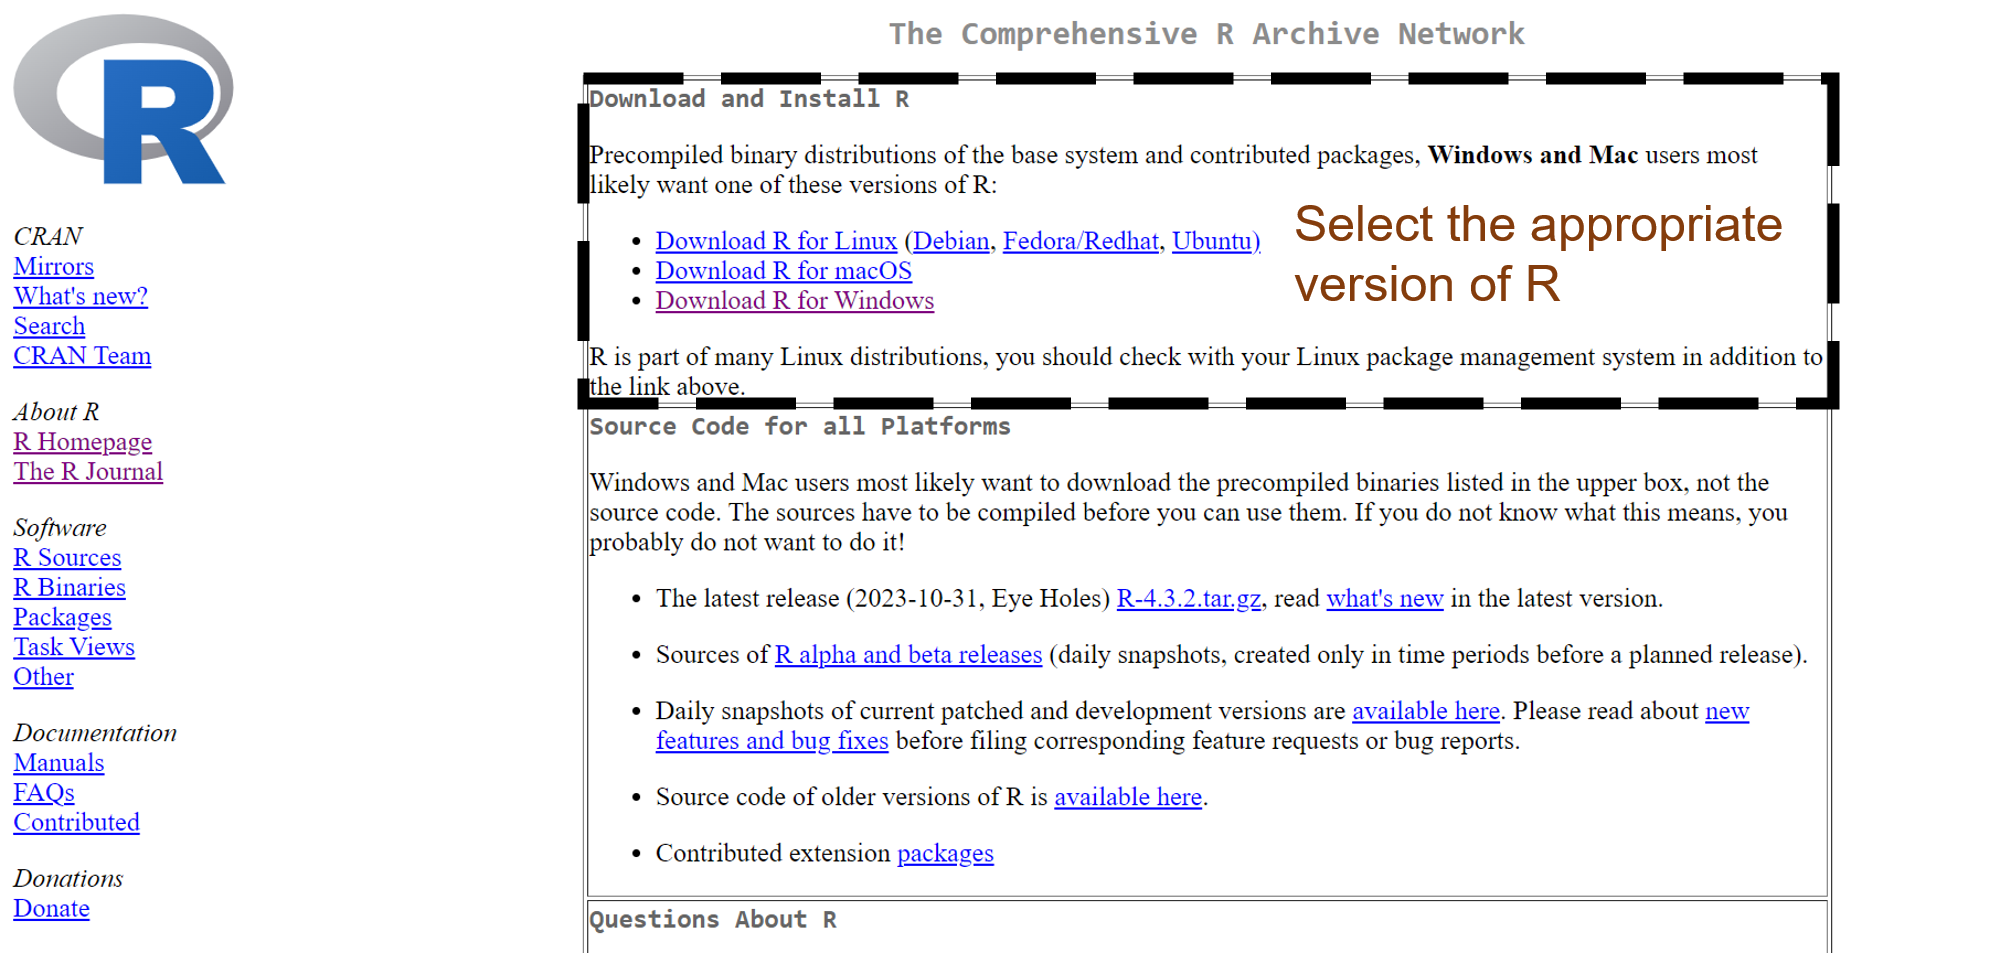
\includegraphics{images/downloading/r_cran_1.png}

}

\caption{\label{fig-cran-1}The CRAN Homepage (Part 1)}

\end{figure}%

\subsubsection{Step 2}\label{step-2}

If installing R for the 1st time, click on ``base''
(Figure~\ref{fig-cran-2}).

\begin{figure}

\centering{

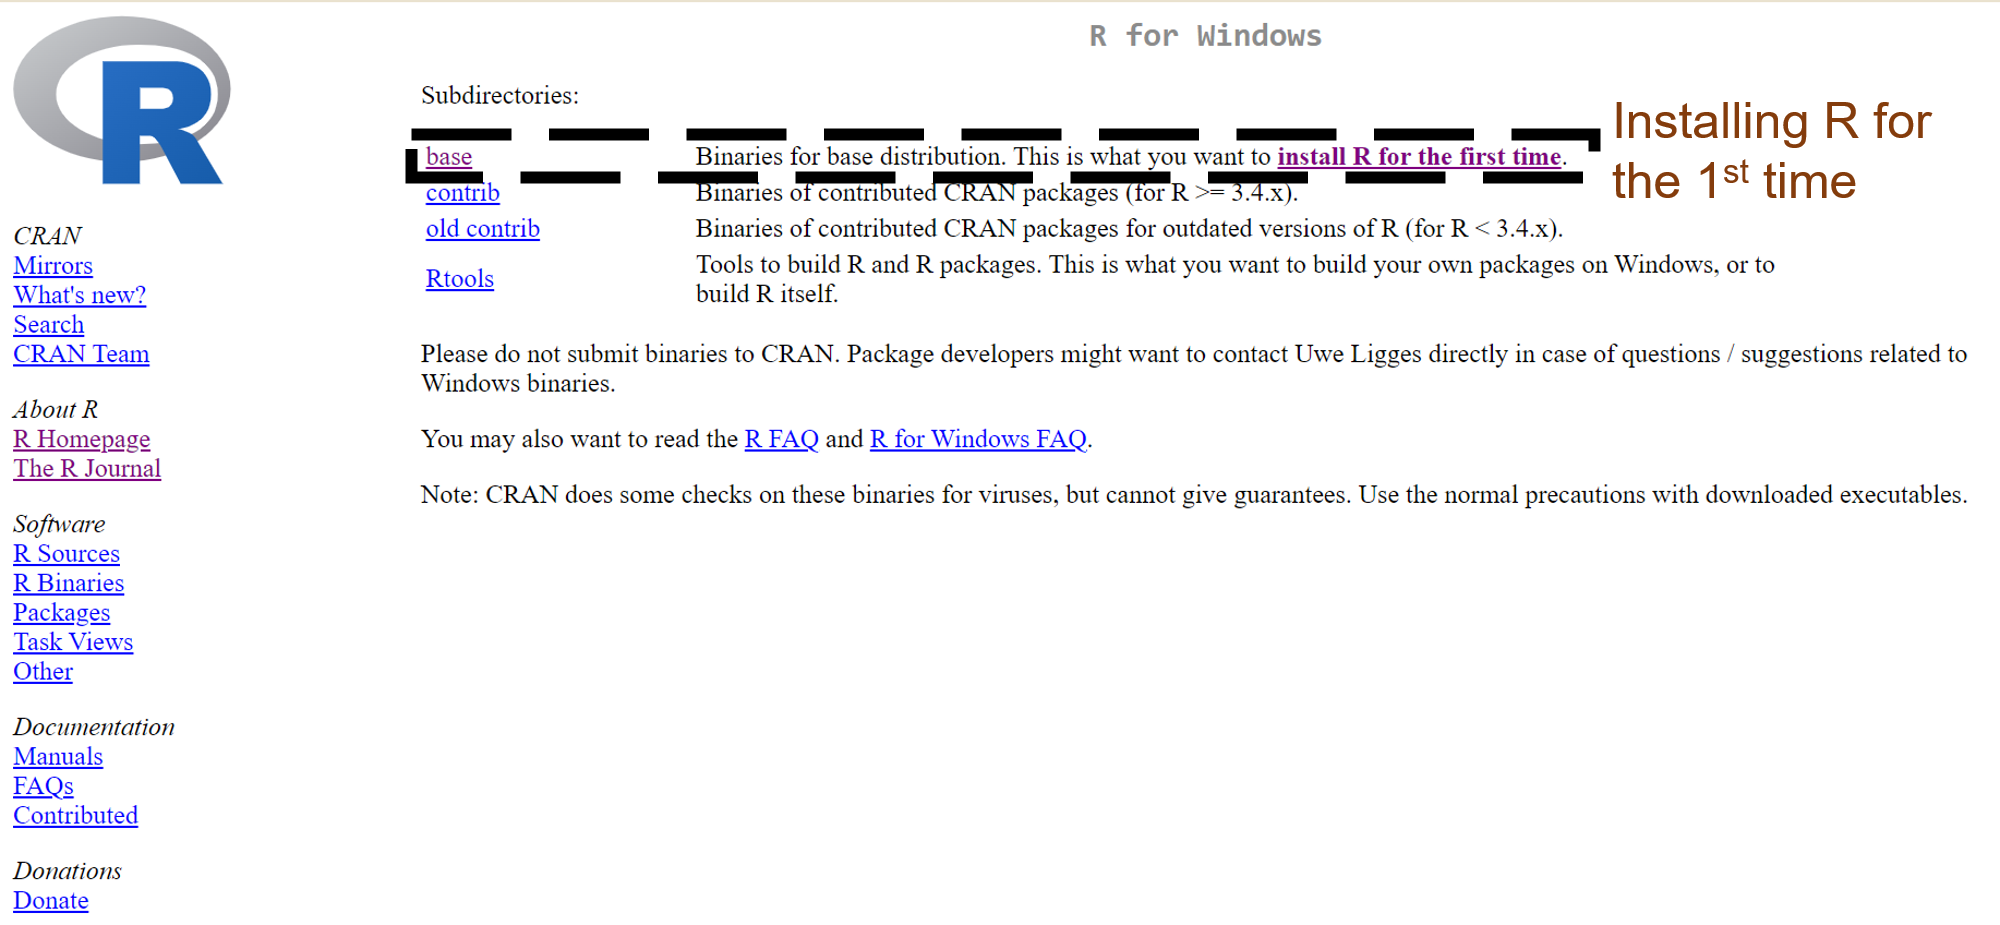
\includegraphics{images/downloading/r_cran_2.png}

}

\caption{\label{fig-cran-2}The CRAN Homepage (Part 2)}

\end{figure}%

\subsubsection{Step 3}\label{step-3}

Click on the ``Download'' link for the latest version of R that is
currently available (at the time of this writing, it was R-4.3.2). Once
downloaded, run the executable file and wait for the software to be
installed (Figure~\ref{fig-cran-3}).

\begin{figure}

\centering{

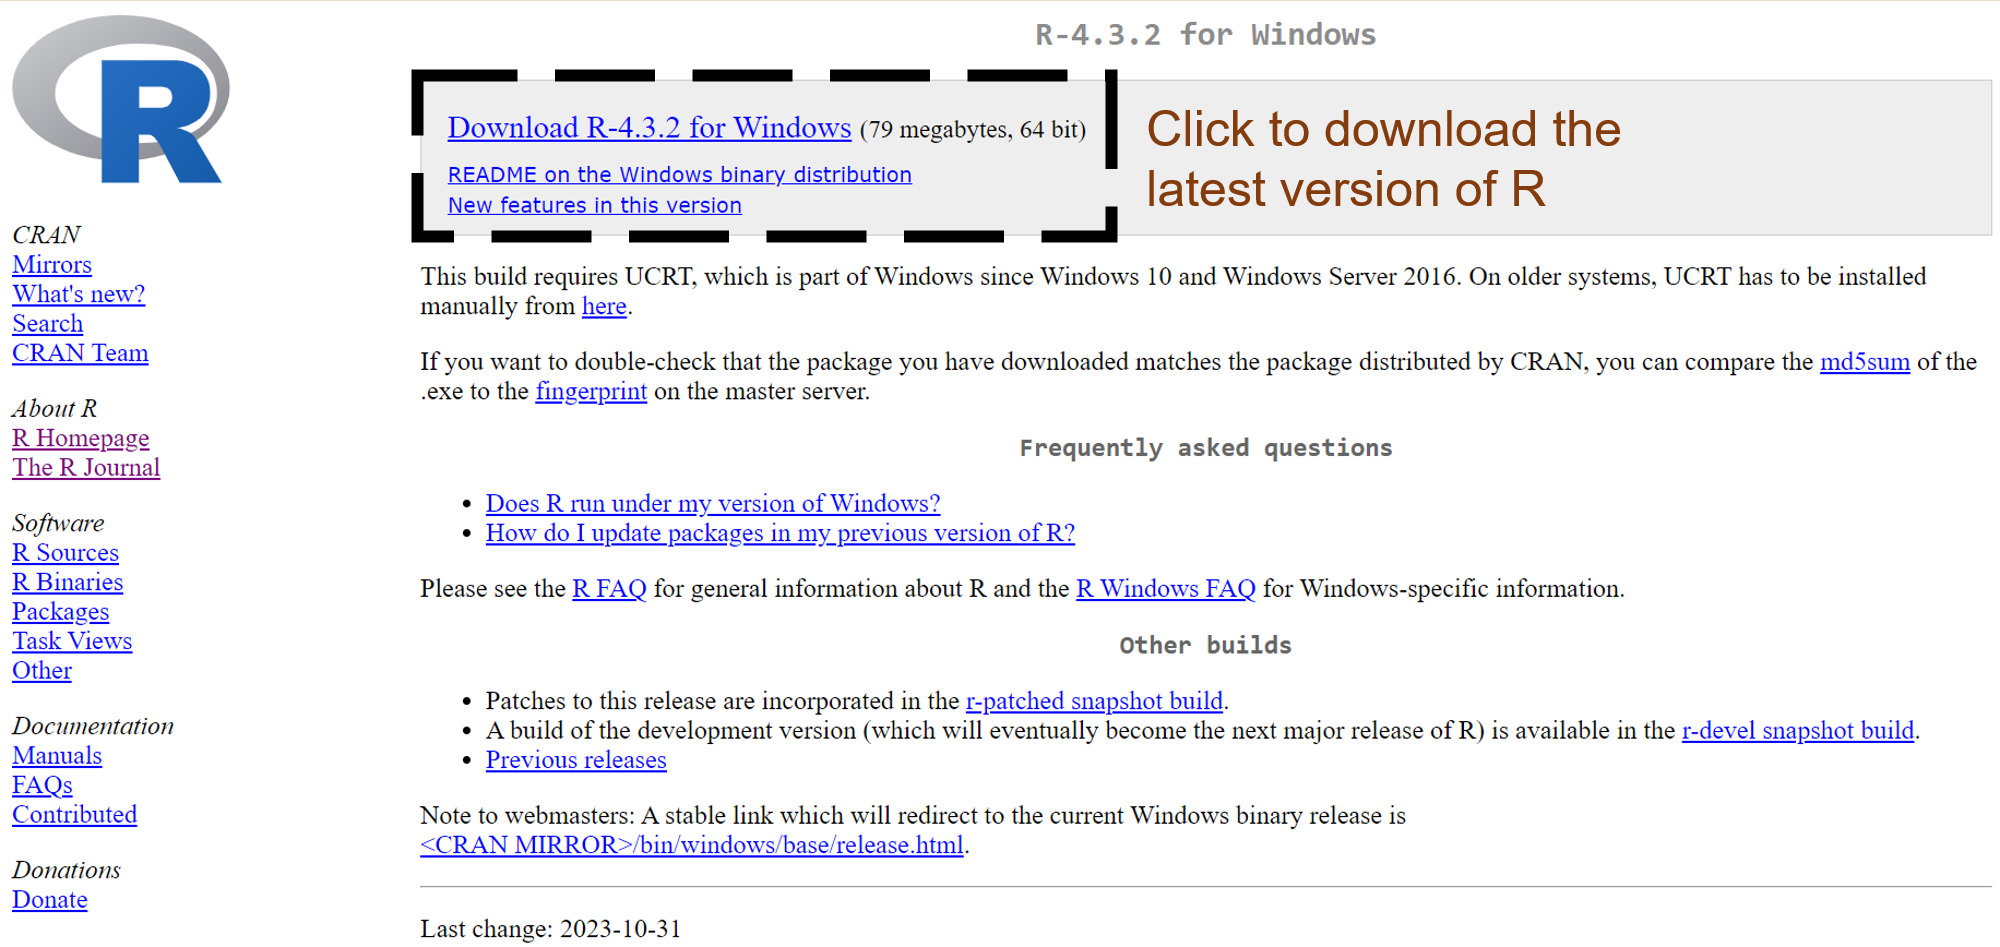
\includegraphics{images/downloading/r_cran_3.png}

}

\caption{\label{fig-cran-3}The CRAN Homepage (Part 3)}

\end{figure}%

\subsubsection{Step 4}\label{step-4}

Once R is installed, open up the R software. The R graphical user
interface should be similar to what is depicted below
(Figure~\ref{fig-r-console-1}).

\begin{figure}

\centering{

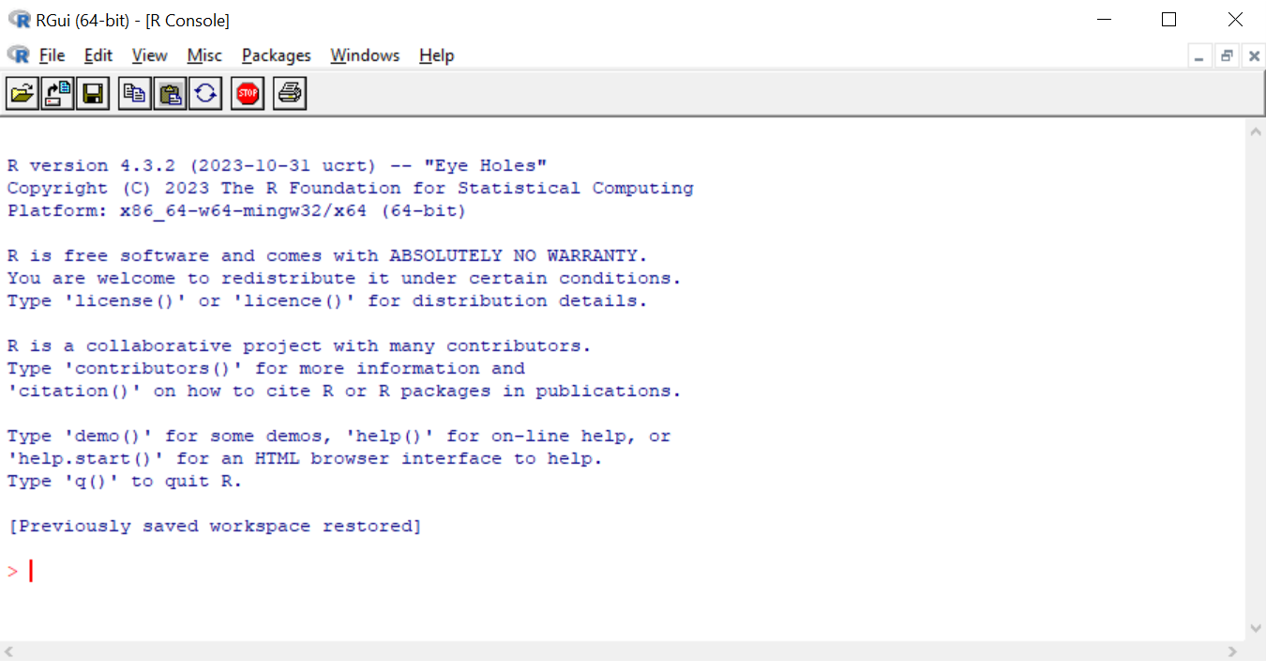
\includegraphics{images/downloading/r_console_1.png}

}

\caption{\label{fig-r-console-1}The R Console}

\end{figure}%

\subsection{Install RStudio}\label{install-rstudio}

The RStudio IDE can be obtained from the ``Download'' section of the
Posit \href{https://posit.co/download/rstudio-desktop/}{website}.
Install the software by clicking on the ``Download RStudio Desktop for
Windows'' button and running the downloaded program
(Figure~\ref{fig-rstudio-1}).

\begin{figure}

\centering{

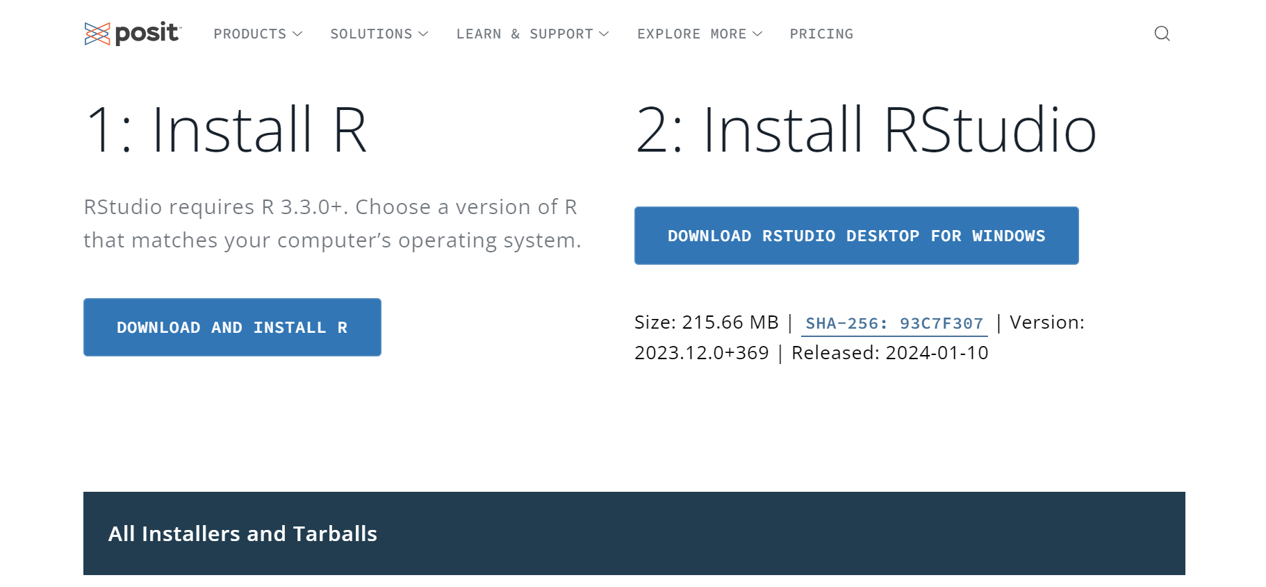
\includegraphics{images/downloading/rstudio_1.png}

}

\caption{\label{fig-rstudio-1}The Posit/RStudio Download Page}

\end{figure}%

Once installed, verify that the RStudio software has a similar graphical
user interface to the one depicted in the image below
(Figure~\ref{fig-rstudio-console-1}).

\begin{figure}

\centering{

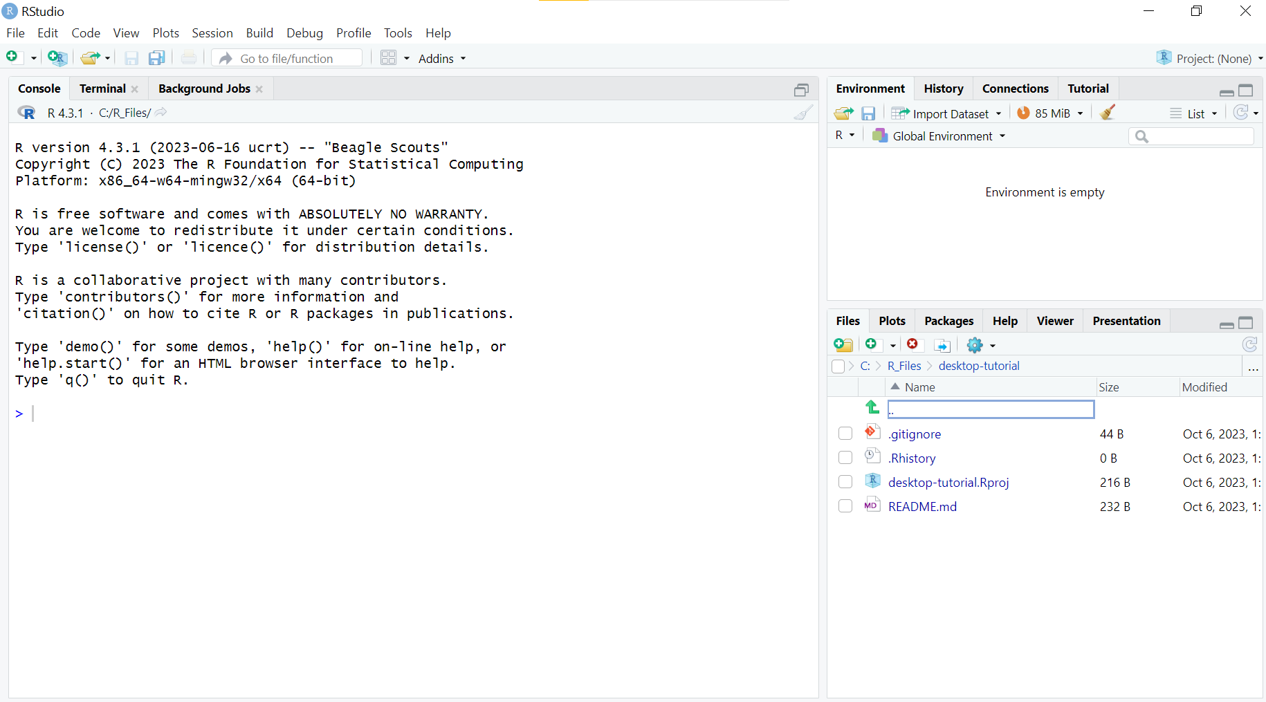
\includegraphics{images/downloading/rstudio_console_1.png}

}

\caption{\label{fig-rstudio-console-1}The RStudio Console}

\end{figure}%

\subsection{Create an RStudio Cloud Account on Posit
website}\label{create-an-rstudio-cloud-account-on-posit-website}

Posit (formerly RStudio) Cloud lets the user access the RStudio
interface from their internet browsers (Figure~\ref{fig-r-cloud-1}).
Using this option does not require any installation or specific software
configuration to be implemented. Posit Cloud offers a
\href{https://posit.cloud/plans/free}{free plan} for casual users
(without the need for a paid plan) and there is no need for dedicated
hardware. Additionally, Posit provides a comprehensive
\href{https://posit.cloud/learn/guide}{guide} for first-time users.

\subsubsection{Step 1}\label{step-1-1}

Access the Posit Cloud Website (Figure~\ref{fig-r-cloud-1}).

\begin{figure}

\centering{


\includegraphics{images/downloading/r_cloud_1.png}

}

\caption{\label{fig-r-cloud-1}The Posit/RStudio Cloud Homepage}

\end{figure}%

\subsubsection{Step 2}\label{step-2-1}

Sign up for a new user account (Figure~\ref{fig-r-cloud-2}).

\begin{figure}

\centering{

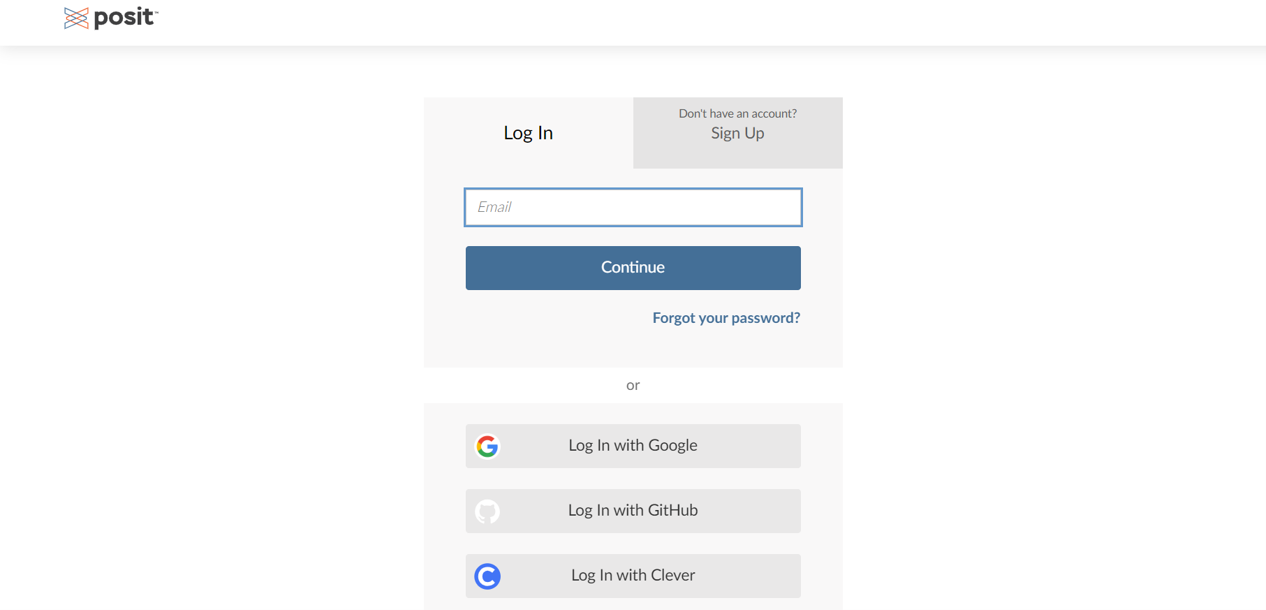
\includegraphics{images/downloading/r_cloud_2.png}

}

\caption{\label{fig-r-cloud-2}The Posit/RStudio Cloud Login Page}

\end{figure}%

\subsubsection{Step 3}\label{step-3-1}

Log in to the new account, and you should see the page shown below
(Figure~\ref{fig-r-cloud-3}). It includes the workspace where all
projects will be hosted. On the top right-hand side of the website is a
button that allows one to create a ``New Project.'' Additionally, the
``Learn'' and ``Help'' sections on the left panel can assist with
troubleshooting.

\begin{figure}

\centering{

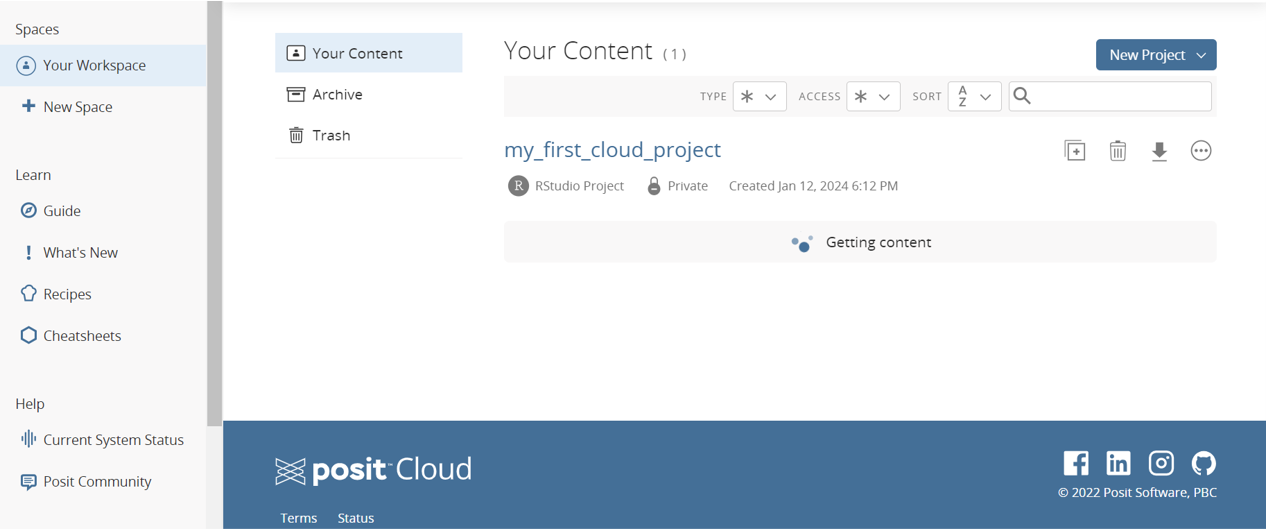
\includegraphics{images/downloading/r_cloud_3.png}

}

\caption{\label{fig-r-cloud-3}The Posit/RStudio Cloud Workspace}

\end{figure}%

\subsubsection{Step 4}\label{step-4-1}

Create an R script to allow for code editing
(Figure~\ref{fig-r-cloud-console-1}).

\begin{figure}

\centering{

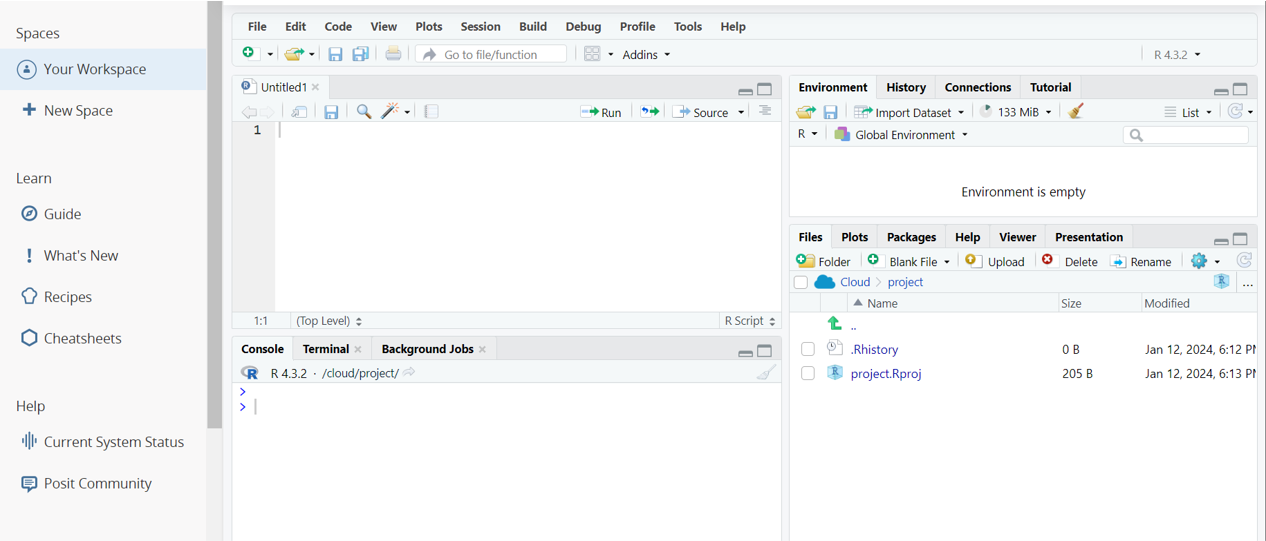
\includegraphics{images/downloading/r_cloud_console_1.png}

}

\caption{\label{fig-r-cloud-console-1}The Posit/RStudio Cloud Console}

\end{figure}%

\subsection{Using alternative code editors to work with R (Advanced
Users)}\label{using-alternative-code-editors-to-work-with-r-advanced-users}

Visual Studio (VS) Code is a code editor that can be used with various
programming languages. For users that have previous experience with this
code editor and would like to use it when reading this book, it is
possible to use VS Code as an alternative to RStudio. After installing
R, the ``R Extension for Visual Studio Code'' can be installed in the
``Extensions'' menu (Figure~\ref{fig-r-vscode}).

\begin{figure}

\centering{

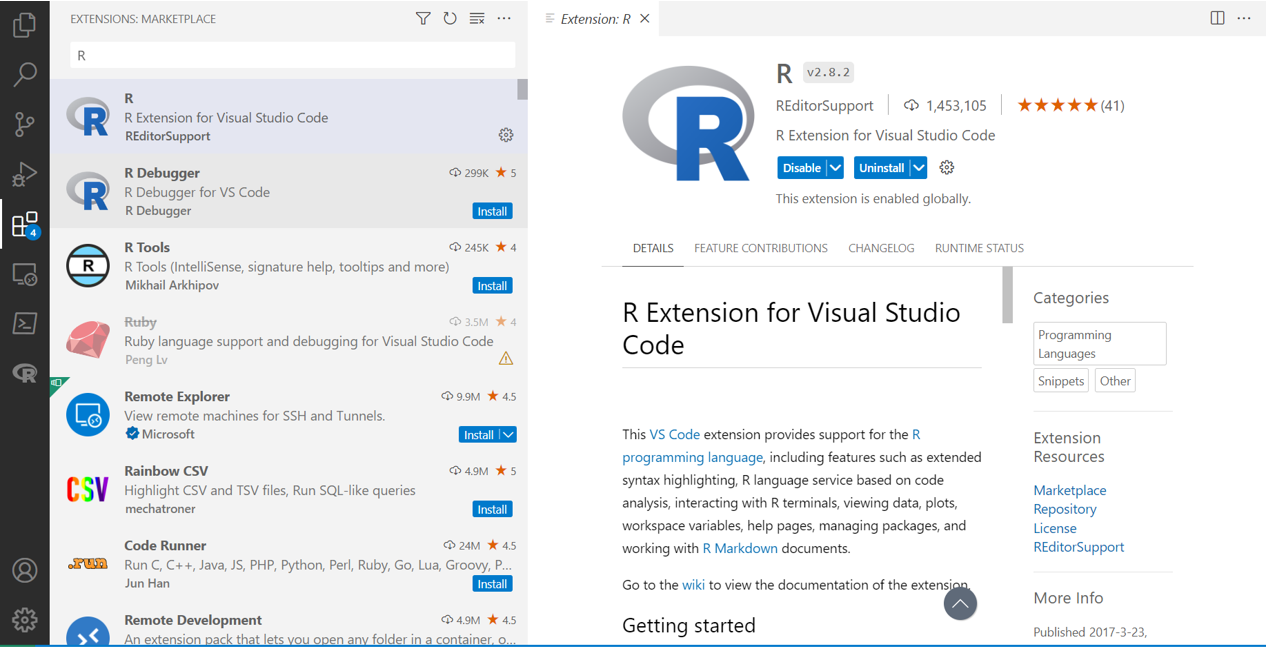
\includegraphics{images/downloading/r_vscode.png}

}

\caption{\label{fig-r-vscode}The R interface on Visual Studio Code}

\end{figure}%

\section{Exercises}\label{exercises-1}

\begin{enumerate}
\def\labelenumi{\roman{enumi}.}
\tightlist
\item
  Download and install R and RStudio (\emph{If you have not already done
  so}).
\item
  Describe the steps involved in installing R on a Windows operating
  system.
\item
  Are there any specific considerations when installing R on a macOS or
  Linux system?
\item
  Set up a free RStudio Cloud Account on the
  \href{https://posit.cloud/}{Posit Website}.
\item
  Compare the local RStudio with the cloud-based RStudio and list the
  potential benefits/disadvantages of both.
\item
  Verify your R installation by running a simple R script that prints
  ``Hello, R! My name is (fill in the blank)'' to the console.
\item
  Can you customize the appearance or behavior of RStudio according to
  your preferences?
\end{enumerate}

\section{Summary}\label{summary-1}

In this chapter, we have provided a step-by-step guide for downloading R
and RStudio on the learner's personal computer. Additionally, the
learner has been shown how to set up an RStudio Cloud account on the
Posit website, which allows for the use of R/RStudio using a web-based
browser. Lastly, the learner has been shown how to access R/RStudio
using alternative code editors such as Visual Studio Code. Overall,
having a functional R and RStudio environment is key to gaining the most
out of your learning journey. In the next chapter, we will navigate the
R/RStudio interfaces and explain the various panes and menu options.

\bookmarksetup{startatroot}

\chapter{Navigating the R and RStudio interfaces}\label{sec-navigating}

\section{Questions}\label{questions-2}

\begin{itemize}
\item
  What are the main components of the R interface?
\item
  How is the RStudio Integrated Development Environment (IDE) organized,
  and what are its key features?
\item
  How does one navigate the R and RStudio interfaces?
\item
  What are the functions of the various RStudio panes?
\end{itemize}

\section{Learning Objectives}\label{learning-objectives-2}

\begin{itemize}
\item
  Identify and understand the main components of the R interface.
\item
  Navigate the RStudio IDE and comprehend its organizational structure.
\item
  Customize your RStudio environment to suit your preferences.
\item
  Understand the roles of the console and menu options in the R
  software.
\item
  Review the various panes and menu options in the RStudio software.
\item
  Learn the various keyboard shortcuts that can improve speed and
  efficiency.
\end{itemize}

\section{Lesson Content}\label{lesson-content-2}

\subsection{The R interface}\label{the-r-interface}

\subsubsection{Menu options}\label{menu-options}

The R graphical user interface opens up with a console where you can
start writing and executing code (Figure~\ref{fig-r-console-1}).
Additionally, there exists a toolbar that contains shortcuts to commonly
used functions. The menu bar allows one to perform various operations
within the R software. The various menu bar options and a brief summary
of their main uses are listed below:

\begin{itemize}
\tightlist
\item
  File: Create new scripts and workspaces, as well as review the session
  history.
\item
  Edit: Copy, paste, and edit, as well as set up the graphical user
  interface (GUI) preferences.
\item
  View: Include the toolbar and status bar within the GUI.
\item
  Misc: Control computations and review objects.
\item
  Packages: Install, load, and update packages.
\item
  Windows: Arrange multiple windows in the learner's preferred
  orientation.
\item
  Help: Find links to FAQs, manuals, and help functions.
\end{itemize}

\begin{figure}

\centering{

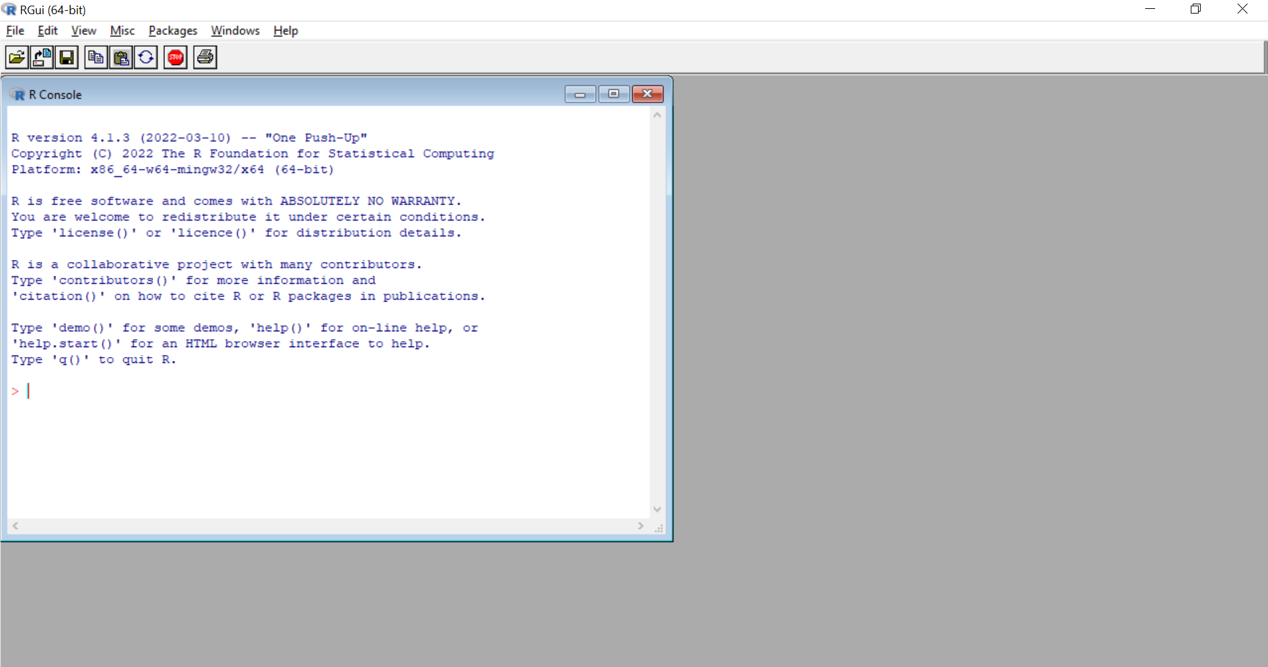
\includegraphics{images/navigating/r_console_1.png}

}

\caption{\label{fig-r-console-1}The R Console}

\end{figure}%

\subsection{RStudio interface (Panes)}\label{rstudio-interface-panes}

When opened for the 1st time, the RStudio interface will have 3 panes:
Console, Environment, and Navigation. To include the 4th required panel,
click on ``File'' --\textgreater{} ``New File'' --\textgreater{} ``R
Script''. Now that the 4 panes are open, let us review their functions.

\subsubsection{Script Pane (Text Editor)}\label{script-pane-text-editor}

The script pane allows the user to write, edit, and save code. This code
can then be run, and the output will be displayed in the console pane.

\subsubsection{Console Pane}\label{console-pane}

In the console pane, one can write and edit code, but not save. Within
the console, one can run one line of code at a time. Additionally, one
can access the terminal tab and run code via the command line. Lastly,
we can access the ``Background Jobs'' tab to monitor progress of R
scripts that are running in a separate, dedicated R session.

\subsubsection{Environment/History Pane}\label{environmenthistory-pane}

This pane has multiple uses. The ``Environment'' tab shows the values of
objects loaded in the current R session. Additionally, from this tab,
one can load workspaces, import datasets, and observe memory usage. The
``History'' tab allows you to see what has been run previously, and the
``Connections'' tab provides a method for connecting to various
databases. Lastly, the ``Tutorial'' tab helps with training users on the
basic concepts of R.

\subsubsection{Navigation Pane}\label{navigation-pane}

The navigation pane allows the user to manage files (create new folders
and scripts), view generated plots, and review and update installed
packages. Additionally, there is a ``Help'' tab for basic queries, and
``Viewer'' and ``Presentation'' tabs for reviewing analysis outputs.

\begin{figure}[H]

{\centering 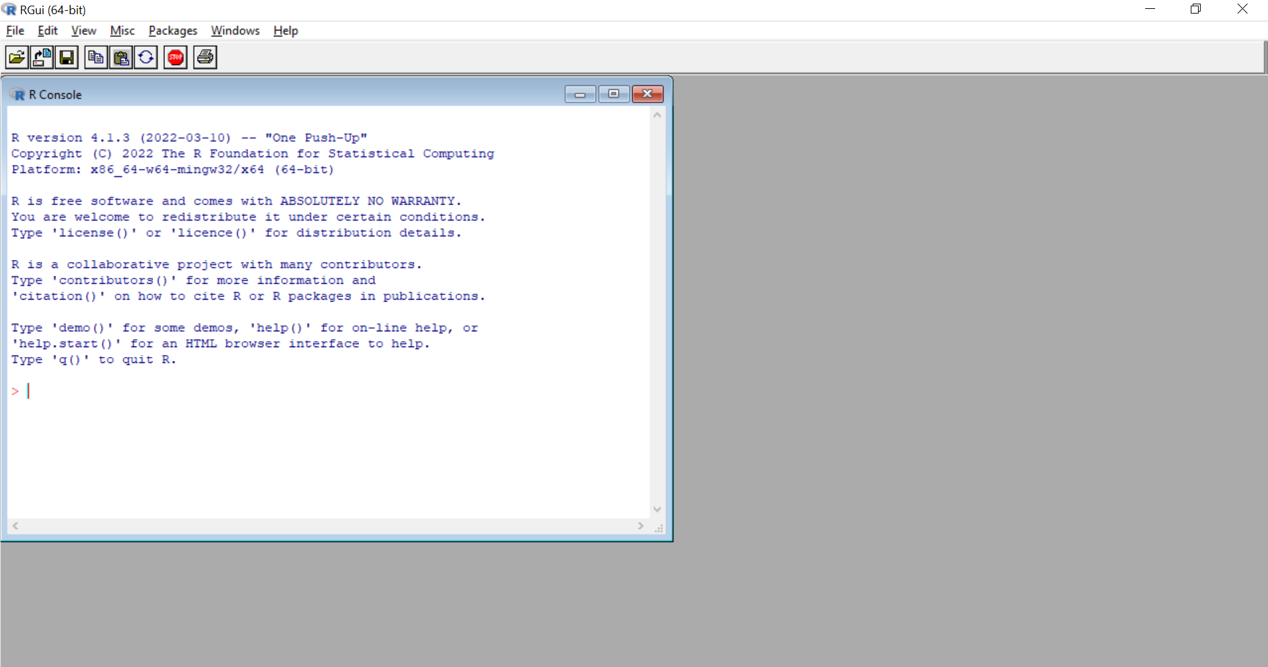
\includegraphics{images/navigating/r_console_1.png}

}

\caption{The R Console}

\end{figure}%

\subsection{RStudio interface (Menu
Options)}\label{rstudio-interface-menu-options}

The RStudio interface has a number of menu bar options
(Figure~\ref{fig-rstudio-console-1}). To orient the user, a brief
description of each menu bar option has been provided below.

\begin{itemize}
\item
  File: Create new files and projects, save them, as well as open and
  close the projects. Additionally, importing of datasets is made much
  easier by the ``Import Dataset'' option.
\item
  Edit: Using this option, one can cut, copy, and paste, as well as undo
  and redo any actions.
\item
  Code: Edit code formats and run code.
\item
  View: Change the appearance of the RStudio graphical user interface
  (GUI), adjust and view different panes.
\item
  Plots: View plots and save the plot outputs to different formats.
\item
  Session: Create sessions, load workspaces, and set the working
  directories.
\item
  Build: Configure build tools and edit the project options.
\item
  Debug: Debug your code.
\item
  \emph{Profile:}
\item
  Help: The help section allows one to access tools for troubleshooting.
  Additionally, it contains documentation and cheatsheets that allow for
  to discover more about the software.
\item
  Tools: Install packages and check for package updates. Additionally,
  one can review version control options, access the terminal, and look
  at keyboard shortcuts. A short snippet of the numerous shortcuts is
  shown below (Figure~\ref{fig-rstudio-ks-1}).
\end{itemize}

\begin{figure}

\centering{

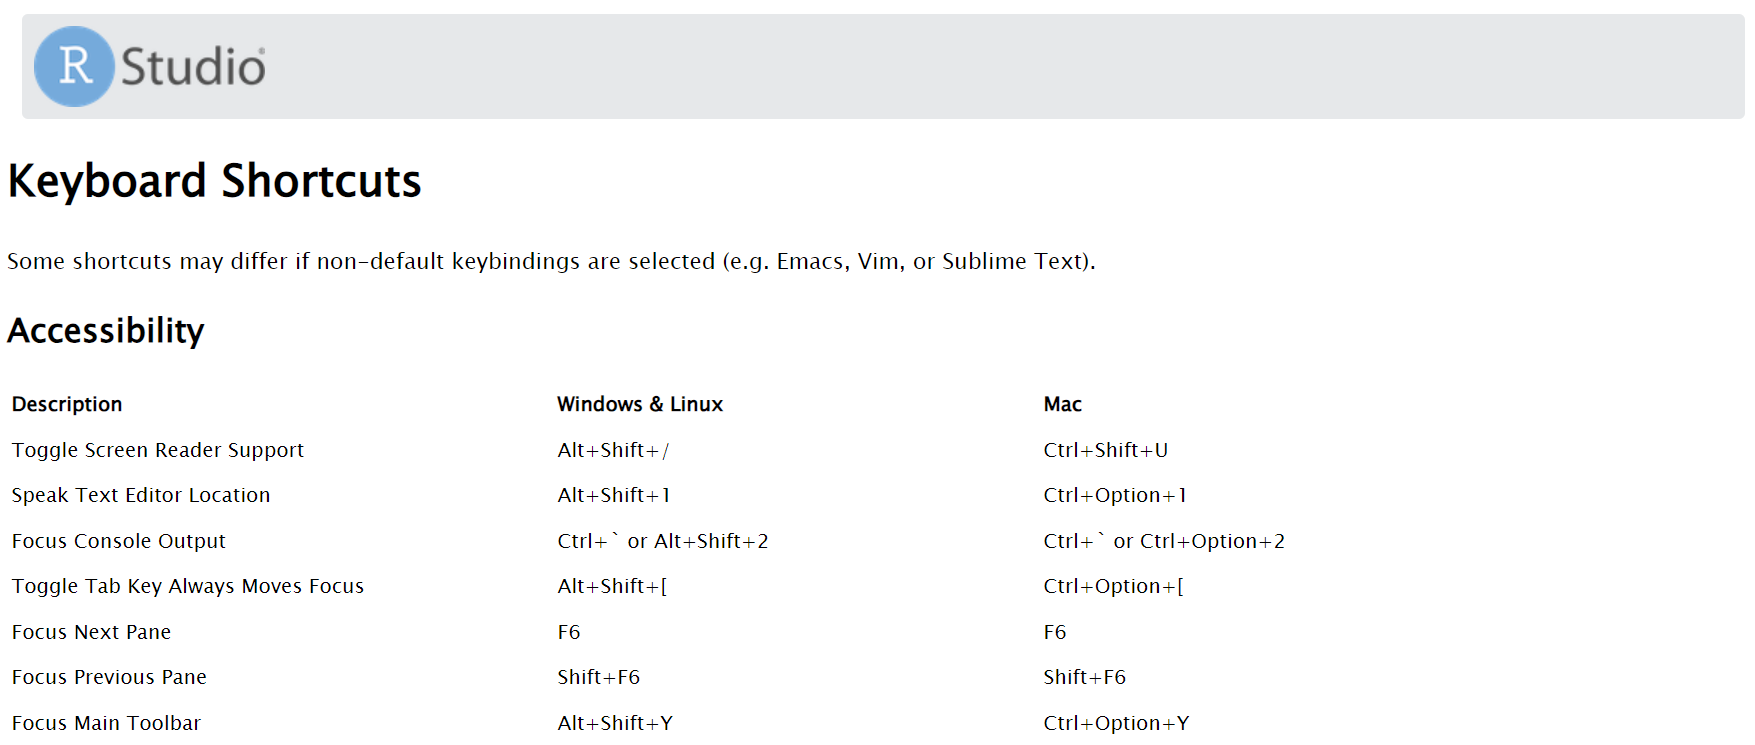
\includegraphics{images/navigating/rstudio_ks_1.png}

}

\caption{\label{fig-rstudio-ks-1}A list of shortcuts available in
RStudio}

\end{figure}%

Lastly, one access both ``Project Options'' and ``Global Options'' from
this menu bar option. Here, the user can change the appearance and pane
layout for individual projects and globally.

\section{Exercises}\label{exercises-2}

\begin{enumerate}
\def\labelenumi{\roman{enumi}.}
\tightlist
\item
  Describe the main components of the RStudio interface.
\item
  Open RStudio and explore the different panels of the interface, then
  describe in your own words the purpose of the Environment, History,
  Files, and Plots panes.
\item
  What is the purpose of the Console pane in RStudio?
\item
  Access the help documentation using the Help pane and find information
  on specific R functions/packages.
\item
  Customize your RStudio environment by changing the theme and adjusting
  the appearance settings.
\item
  Practice using keyboard shortcuts for common tasks in RStudio.
\item
  How can you customize the layout of panes in RStudio?
\end{enumerate}

\section{Summary}\label{summary-2}

This brief overview of the R/RStudio interface should make the learner
more comfortable when using the software. In this chapter, we explored
the main components of the R interface and delved into the
organizational structure of the RStudio IDE. Understanding the different
panes and tabs within RStudio is crucial for efficient and effective
programming. We navigated through the Source, Console, Environment,
Plots, and Help panes, as well as additional tabs for managing files,
plots, packages, and the viewer. Customizing your RStudio environment
enhances your overall experience, and practicing keyboard shortcuts can
significantly improve your coding efficiency. As you proceed with this
guide, having a solid grasp of navigating the R and RStudio interfaces
will empower you in your journey as an R programmer. Few introductory
courses provide this overview, and it is hoped that this will decrease
the cognitive load on learners in future lessons.

\bookmarksetup{startatroot}

\chapter{Managing your files and data}\label{sec-managing}

\section{Questions}\label{questions-3}

\begin{itemize}
\item
  Why is good file and data management important in R?
\item
  What is the concept of a project in R, and how does it help in
  organizing your work?
\item
  What is the purpose of creating R project folders and scripts?
\item
  What is the significance of a working directory in R, and how does it
  impact your workflow?
\item
  How do you create, save, and run R scripts for efficient code
  management?
\end{itemize}

\section{Learning Objectives}\label{learning-objectives-3}

\begin{itemize}
\item
  Understand the importance of properly organized files and datasets for
  efficient R projects.
\item
  Understand the concept of R projects and their role in organizing your
  work.
\item
  Write and run R code in scripts for better code organization and
  reproducibility.
\item
  Master the concept of working directories and navigate your project
  files effectively.
\end{itemize}

\section{Lesson Content}\label{lesson-content-3}

\subsection{Introduction}\label{introduction-2}

Good file and data management allows the user to debug code, reduce the
number of coding errors, and improve data quality. Additionally, by
utilizing best practices the learner can easily share their work,
organize projects, and develop a reproducible workflow.

\subsection{Projects}\label{projects}

An R project enables the learner to keep all their work in one folder.
In the R project folder, all scripts, data files, figures, tables,
history, and output can be stored in sub-folders within the R project.
The root folder of the project is also known as the working directory
(described in the section below).

To create a new project folder:

File --\textgreater{} New Project

\subsection{Scripts}\label{scripts}

To ensure that the learner has a record of all the code that they have
written in the console, it is important that the learner also write the
code in a script and saves it. Failure to do this will mean that the
learner will have to write the code in the console every time they need
to execute it. Code written in script files allows one to run it
multiple times and edit when necessary.

To create a new script file:

File --\textgreater{} New File --\textgreater{} R Script

Save the file in your project folder

Ensure that the file names are readable for both the R software and
collaborators.

Examples include:

\begin{itemize}
\tightlist
\item
  ``my\_model\_1.R''
\end{itemize}

\subsection{Working Directory}\label{working-directory}

The working directory is a file path or location on your computer that R
uses for reading and writing files. The function \texttt{getwd()} prints
the current working directory, and \texttt{setwd()} allows the user to
set the working directory. This is where R looks for files that you ask
it to load, and where it puts any files that you ask it to save.

The paths to files or directories can be defined using relative or
absolute paths. The relative path is where the file is found in the
location where the user is, and absolute includes the entire path from
the root directory.

\subsection{Finding help when using packages and
functions}\label{finding-help-when-using-packages-and-functions}

\begin{itemize}
\item
  There is a built-in help system that can be accessed via the ``Help''
  menu or one can use the \texttt{?} symbol before the function,
  package, or dataset to get a brief description and instructions for
  use.
\item
  Online R \href{https://cran.r-project.org/manuals.html}{documentation}
  is also available to allow the user to learn the basics of R.
\end{itemize}

\section{Exercises}\label{exercises-3}

\begin{enumerate}
\def\labelenumi{\roman{enumi}.}
\item
  Create a new RStudio project called ``novice\_programmer\_guide''.
\item
  Within the project folder, create a new R Script called
  ``introduction.R'' and save it.
\item
  Set your working directory in the console to the root of this new
  project, and practice loading data from a file within it.
\item
  Explain the significance of using relative and absolute file paths in
  R, and experiment with using relative paths to access different data
  files within your project directory.
\item
  Explain the role of the functions, \texttt{file.path()},
  \texttt{list.files()}, and \texttt{dir.create()}, in R.
\item
  Describe the purpose of the \texttt{.Rproj} file in an R project.
\item
  How can you clear the R workspace? Explore functions like
  \texttt{rm()} and \texttt{rm(list=ls())} to remove unwanted objects.
\end{enumerate}

\section{Summary}\label{summary-3}

Hopefully, this lesson has demonstrated to the learner the importance of
good file and data management. We have reviewed the concepts of
projects, scripts, and working directories and shown how this can help
with file organization, saving/reusing code, and ultimately impact
project reproducibility. In the next lesson, we will see how this is
important when importing data and saving analysis outputs.

\bookmarksetup{startatroot}

\chapter{Importing data and saving analysis
outputs}\label{sec-import-save}

\section{Questions}\label{questions-4}

\begin{itemize}
\item
  Can users access and use internal datasets for analysis in R? How do I
  load the datasets?
\item
  How does one import external datasets into R? What functions and
  packages are commonly used for this purpose?
\item
  How do I handle different data formats such as CSV, Excel, or text
  files?
\item
  Once the user completes their data analysis, how can their output(s)
  be saved?
\item
  How can I create new data objects or modify existing ones within R?
\end{itemize}

\section{Learning Objectives}\label{learning-objectives-4}

\begin{itemize}
\item
  Learn how to load and access internal R datasets.
\item
  Import external datasets into your R project folder.
\item
  Demonstrate how to save analysis outputs from R such as tables and
  datasets.
\item
  Understand methods for importing data stored internally in R and from
  external sources.
\item
  Utilize built-in functions and packages to read various data formats
  like CSV, Excel, and text files.
\end{itemize}

\section{Lesson Content}\label{lesson-content-4}

\subsection{Introduction}\label{introduction-3}

A dataset is a collection of data, and R offers the user the opportunity
to either use internal datasets or import external datasets for
analysis. In this lesson, we will cover the basics of accessing internal
datasets, the importation of external datasets, as well as the saving of
analysis outputs, such as plots and tables.

\subsection{Working with internal
datasets}\label{working-with-internal-datasets}

R has several built-in datasets. To access them, we use the
\texttt{data()} function after loading in the datasets library.

\begin{Shaded}
\begin{Highlighting}[]
\FunctionTok{library}\NormalTok{(datasets)}

\FunctionTok{print}\NormalTok{(}\FunctionTok{data}\NormalTok{())}
\end{Highlighting}
\end{Shaded}

To find out more about a specific dataset, we use the \texttt{?}
operator.

\texttt{?dataset}

Example:

\begin{Shaded}
\begin{Highlighting}[]
\FunctionTok{print}\NormalTok{(?airquality)}
\end{Highlighting}
\end{Shaded}

\begin{verbatim}
starting httpd help server ... done
\end{verbatim}

\textbf{Helpful functions when working with datasets}

\subsubsection{Loading datasets}\label{loading-datasets}

\texttt{datasets::dataset}

OR

\texttt{datasets("dataset")}

Example:

\begin{Shaded}
\begin{Highlighting}[]
\NormalTok{datasets}\SpecialCharTok{::}\NormalTok{airquality}
\end{Highlighting}
\end{Shaded}

\begin{verbatim}
    Ozone Solar.R Wind Temp Month Day
1      41     190  7.4   67     5   1
2      36     118  8.0   72     5   2
3      12     149 12.6   74     5   3
4      18     313 11.5   62     5   4
5      NA      NA 14.3   56     5   5
6      28      NA 14.9   66     5   6
7      23     299  8.6   65     5   7
8      19      99 13.8   59     5   8
9       8      19 20.1   61     5   9
10     NA     194  8.6   69     5  10
11      7      NA  6.9   74     5  11
12     16     256  9.7   69     5  12
13     11     290  9.2   66     5  13
14     14     274 10.9   68     5  14
15     18      65 13.2   58     5  15
16     14     334 11.5   64     5  16
17     34     307 12.0   66     5  17
18      6      78 18.4   57     5  18
19     30     322 11.5   68     5  19
20     11      44  9.7   62     5  20
21      1       8  9.7   59     5  21
22     11     320 16.6   73     5  22
23      4      25  9.7   61     5  23
24     32      92 12.0   61     5  24
25     NA      66 16.6   57     5  25
26     NA     266 14.9   58     5  26
27     NA      NA  8.0   57     5  27
28     23      13 12.0   67     5  28
29     45     252 14.9   81     5  29
30    115     223  5.7   79     5  30
31     37     279  7.4   76     5  31
32     NA     286  8.6   78     6   1
33     NA     287  9.7   74     6   2
34     NA     242 16.1   67     6   3
35     NA     186  9.2   84     6   4
36     NA     220  8.6   85     6   5
37     NA     264 14.3   79     6   6
38     29     127  9.7   82     6   7
39     NA     273  6.9   87     6   8
40     71     291 13.8   90     6   9
41     39     323 11.5   87     6  10
42     NA     259 10.9   93     6  11
43     NA     250  9.2   92     6  12
44     23     148  8.0   82     6  13
45     NA     332 13.8   80     6  14
46     NA     322 11.5   79     6  15
47     21     191 14.9   77     6  16
48     37     284 20.7   72     6  17
49     20      37  9.2   65     6  18
50     12     120 11.5   73     6  19
51     13     137 10.3   76     6  20
52     NA     150  6.3   77     6  21
53     NA      59  1.7   76     6  22
54     NA      91  4.6   76     6  23
55     NA     250  6.3   76     6  24
56     NA     135  8.0   75     6  25
57     NA     127  8.0   78     6  26
58     NA      47 10.3   73     6  27
59     NA      98 11.5   80     6  28
60     NA      31 14.9   77     6  29
61     NA     138  8.0   83     6  30
62    135     269  4.1   84     7   1
63     49     248  9.2   85     7   2
64     32     236  9.2   81     7   3
65     NA     101 10.9   84     7   4
66     64     175  4.6   83     7   5
67     40     314 10.9   83     7   6
68     77     276  5.1   88     7   7
69     97     267  6.3   92     7   8
70     97     272  5.7   92     7   9
71     85     175  7.4   89     7  10
72     NA     139  8.6   82     7  11
73     10     264 14.3   73     7  12
74     27     175 14.9   81     7  13
75     NA     291 14.9   91     7  14
76      7      48 14.3   80     7  15
77     48     260  6.9   81     7  16
78     35     274 10.3   82     7  17
79     61     285  6.3   84     7  18
80     79     187  5.1   87     7  19
81     63     220 11.5   85     7  20
82     16       7  6.9   74     7  21
83     NA     258  9.7   81     7  22
84     NA     295 11.5   82     7  23
85     80     294  8.6   86     7  24
86    108     223  8.0   85     7  25
87     20      81  8.6   82     7  26
88     52      82 12.0   86     7  27
89     82     213  7.4   88     7  28
90     50     275  7.4   86     7  29
91     64     253  7.4   83     7  30
92     59     254  9.2   81     7  31
93     39      83  6.9   81     8   1
94      9      24 13.8   81     8   2
95     16      77  7.4   82     8   3
96     78      NA  6.9   86     8   4
97     35      NA  7.4   85     8   5
98     66      NA  4.6   87     8   6
99    122     255  4.0   89     8   7
100    89     229 10.3   90     8   8
101   110     207  8.0   90     8   9
102    NA     222  8.6   92     8  10
103    NA     137 11.5   86     8  11
104    44     192 11.5   86     8  12
105    28     273 11.5   82     8  13
106    65     157  9.7   80     8  14
107    NA      64 11.5   79     8  15
108    22      71 10.3   77     8  16
109    59      51  6.3   79     8  17
110    23     115  7.4   76     8  18
111    31     244 10.9   78     8  19
112    44     190 10.3   78     8  20
113    21     259 15.5   77     8  21
114     9      36 14.3   72     8  22
115    NA     255 12.6   75     8  23
116    45     212  9.7   79     8  24
117   168     238  3.4   81     8  25
118    73     215  8.0   86     8  26
119    NA     153  5.7   88     8  27
120    76     203  9.7   97     8  28
121   118     225  2.3   94     8  29
122    84     237  6.3   96     8  30
123    85     188  6.3   94     8  31
124    96     167  6.9   91     9   1
125    78     197  5.1   92     9   2
126    73     183  2.8   93     9   3
127    91     189  4.6   93     9   4
128    47      95  7.4   87     9   5
129    32      92 15.5   84     9   6
130    20     252 10.9   80     9   7
131    23     220 10.3   78     9   8
132    21     230 10.9   75     9   9
133    24     259  9.7   73     9  10
134    44     236 14.9   81     9  11
135    21     259 15.5   76     9  12
136    28     238  6.3   77     9  13
137     9      24 10.9   71     9  14
138    13     112 11.5   71     9  15
139    46     237  6.9   78     9  16
140    18     224 13.8   67     9  17
141    13      27 10.3   76     9  18
142    24     238 10.3   68     9  19
143    16     201  8.0   82     9  20
144    13     238 12.6   64     9  21
145    23      14  9.2   71     9  22
146    36     139 10.3   81     9  23
147     7      49 10.3   69     9  24
148    14      20 16.6   63     9  25
149    30     193  6.9   70     9  26
150    NA     145 13.2   77     9  27
151    14     191 14.3   75     9  28
152    18     131  8.0   76     9  29
153    20     223 11.5   68     9  30
\end{verbatim}

\begin{Shaded}
\begin{Highlighting}[]
\FunctionTok{data}\NormalTok{(}\StringTok{"airquality"}\NormalTok{)}
\end{Highlighting}
\end{Shaded}

\subsubsection{Print datasets}\label{print-datasets}

\texttt{print(dataset)}

Example:

\begin{Shaded}
\begin{Highlighting}[]
\FunctionTok{print}\NormalTok{(airquality)}
\end{Highlighting}
\end{Shaded}

\begin{verbatim}
    Ozone Solar.R Wind Temp Month Day
1      41     190  7.4   67     5   1
2      36     118  8.0   72     5   2
3      12     149 12.6   74     5   3
4      18     313 11.5   62     5   4
5      NA      NA 14.3   56     5   5
6      28      NA 14.9   66     5   6
7      23     299  8.6   65     5   7
8      19      99 13.8   59     5   8
9       8      19 20.1   61     5   9
10     NA     194  8.6   69     5  10
11      7      NA  6.9   74     5  11
12     16     256  9.7   69     5  12
13     11     290  9.2   66     5  13
14     14     274 10.9   68     5  14
15     18      65 13.2   58     5  15
16     14     334 11.5   64     5  16
17     34     307 12.0   66     5  17
18      6      78 18.4   57     5  18
19     30     322 11.5   68     5  19
20     11      44  9.7   62     5  20
21      1       8  9.7   59     5  21
22     11     320 16.6   73     5  22
23      4      25  9.7   61     5  23
24     32      92 12.0   61     5  24
25     NA      66 16.6   57     5  25
26     NA     266 14.9   58     5  26
27     NA      NA  8.0   57     5  27
28     23      13 12.0   67     5  28
29     45     252 14.9   81     5  29
30    115     223  5.7   79     5  30
31     37     279  7.4   76     5  31
32     NA     286  8.6   78     6   1
33     NA     287  9.7   74     6   2
34     NA     242 16.1   67     6   3
35     NA     186  9.2   84     6   4
36     NA     220  8.6   85     6   5
37     NA     264 14.3   79     6   6
38     29     127  9.7   82     6   7
39     NA     273  6.9   87     6   8
40     71     291 13.8   90     6   9
41     39     323 11.5   87     6  10
42     NA     259 10.9   93     6  11
43     NA     250  9.2   92     6  12
44     23     148  8.0   82     6  13
45     NA     332 13.8   80     6  14
46     NA     322 11.5   79     6  15
47     21     191 14.9   77     6  16
48     37     284 20.7   72     6  17
49     20      37  9.2   65     6  18
50     12     120 11.5   73     6  19
51     13     137 10.3   76     6  20
52     NA     150  6.3   77     6  21
53     NA      59  1.7   76     6  22
54     NA      91  4.6   76     6  23
55     NA     250  6.3   76     6  24
56     NA     135  8.0   75     6  25
57     NA     127  8.0   78     6  26
58     NA      47 10.3   73     6  27
59     NA      98 11.5   80     6  28
60     NA      31 14.9   77     6  29
61     NA     138  8.0   83     6  30
62    135     269  4.1   84     7   1
63     49     248  9.2   85     7   2
64     32     236  9.2   81     7   3
65     NA     101 10.9   84     7   4
66     64     175  4.6   83     7   5
67     40     314 10.9   83     7   6
68     77     276  5.1   88     7   7
69     97     267  6.3   92     7   8
70     97     272  5.7   92     7   9
71     85     175  7.4   89     7  10
72     NA     139  8.6   82     7  11
73     10     264 14.3   73     7  12
74     27     175 14.9   81     7  13
75     NA     291 14.9   91     7  14
76      7      48 14.3   80     7  15
77     48     260  6.9   81     7  16
78     35     274 10.3   82     7  17
79     61     285  6.3   84     7  18
80     79     187  5.1   87     7  19
81     63     220 11.5   85     7  20
82     16       7  6.9   74     7  21
83     NA     258  9.7   81     7  22
84     NA     295 11.5   82     7  23
85     80     294  8.6   86     7  24
86    108     223  8.0   85     7  25
87     20      81  8.6   82     7  26
88     52      82 12.0   86     7  27
89     82     213  7.4   88     7  28
90     50     275  7.4   86     7  29
91     64     253  7.4   83     7  30
92     59     254  9.2   81     7  31
93     39      83  6.9   81     8   1
94      9      24 13.8   81     8   2
95     16      77  7.4   82     8   3
96     78      NA  6.9   86     8   4
97     35      NA  7.4   85     8   5
98     66      NA  4.6   87     8   6
99    122     255  4.0   89     8   7
100    89     229 10.3   90     8   8
101   110     207  8.0   90     8   9
102    NA     222  8.6   92     8  10
103    NA     137 11.5   86     8  11
104    44     192 11.5   86     8  12
105    28     273 11.5   82     8  13
106    65     157  9.7   80     8  14
107    NA      64 11.5   79     8  15
108    22      71 10.3   77     8  16
109    59      51  6.3   79     8  17
110    23     115  7.4   76     8  18
111    31     244 10.9   78     8  19
112    44     190 10.3   78     8  20
113    21     259 15.5   77     8  21
114     9      36 14.3   72     8  22
115    NA     255 12.6   75     8  23
116    45     212  9.7   79     8  24
117   168     238  3.4   81     8  25
118    73     215  8.0   86     8  26
119    NA     153  5.7   88     8  27
120    76     203  9.7   97     8  28
121   118     225  2.3   94     8  29
122    84     237  6.3   96     8  30
123    85     188  6.3   94     8  31
124    96     167  6.9   91     9   1
125    78     197  5.1   92     9   2
126    73     183  2.8   93     9   3
127    91     189  4.6   93     9   4
128    47      95  7.4   87     9   5
129    32      92 15.5   84     9   6
130    20     252 10.9   80     9   7
131    23     220 10.3   78     9   8
132    21     230 10.9   75     9   9
133    24     259  9.7   73     9  10
134    44     236 14.9   81     9  11
135    21     259 15.5   76     9  12
136    28     238  6.3   77     9  13
137     9      24 10.9   71     9  14
138    13     112 11.5   71     9  15
139    46     237  6.9   78     9  16
140    18     224 13.8   67     9  17
141    13      27 10.3   76     9  18
142    24     238 10.3   68     9  19
143    16     201  8.0   82     9  20
144    13     238 12.6   64     9  21
145    23      14  9.2   71     9  22
146    36     139 10.3   81     9  23
147     7      49 10.3   69     9  24
148    14      20 16.6   63     9  25
149    30     193  6.9   70     9  26
150    NA     145 13.2   77     9  27
151    14     191 14.3   75     9  28
152    18     131  8.0   76     9  29
153    20     223 11.5   68     9  30
\end{verbatim}

\subsubsection{Inspect head and tail of
datasets}\label{inspect-head-and-tail-of-datasets}

\texttt{head(dataset)}

OR

\texttt{tail(dataset)}

Example:

\begin{Shaded}
\begin{Highlighting}[]
\FunctionTok{head}\NormalTok{(airquality)}
\end{Highlighting}
\end{Shaded}

\begin{verbatim}
  Ozone Solar.R Wind Temp Month Day
1    41     190  7.4   67     5   1
2    36     118  8.0   72     5   2
3    12     149 12.6   74     5   3
4    18     313 11.5   62     5   4
5    NA      NA 14.3   56     5   5
6    28      NA 14.9   66     5   6
\end{verbatim}

\begin{Shaded}
\begin{Highlighting}[]
\FunctionTok{tail}\NormalTok{(airquality)}
\end{Highlighting}
\end{Shaded}

\begin{verbatim}
    Ozone Solar.R Wind Temp Month Day
148    14      20 16.6   63     9  25
149    30     193  6.9   70     9  26
150    NA     145 13.2   77     9  27
151    14     191 14.3   75     9  28
152    18     131  8.0   76     9  29
153    20     223 11.5   68     9  30
\end{verbatim}

\subsubsection{Inspect the column and row names in the
dataset}\label{inspect-the-column-and-row-names-in-the-dataset}

Names

\texttt{names(dataset)}

Row names

\texttt{rownames(dataset)}

Column names

\texttt{colnames(dataset)}

Example:

\begin{Shaded}
\begin{Highlighting}[]
\FunctionTok{names}\NormalTok{(airquality)}
\end{Highlighting}
\end{Shaded}

\begin{verbatim}
[1] "Ozone"   "Solar.R" "Wind"    "Temp"    "Month"   "Day"    
\end{verbatim}

\begin{Shaded}
\begin{Highlighting}[]
\FunctionTok{rownames}\NormalTok{(airquality)}
\end{Highlighting}
\end{Shaded}

\begin{verbatim}
  [1] "1"   "2"   "3"   "4"   "5"   "6"   "7"   "8"   "9"   "10"  "11"  "12" 
 [13] "13"  "14"  "15"  "16"  "17"  "18"  "19"  "20"  "21"  "22"  "23"  "24" 
 [25] "25"  "26"  "27"  "28"  "29"  "30"  "31"  "32"  "33"  "34"  "35"  "36" 
 [37] "37"  "38"  "39"  "40"  "41"  "42"  "43"  "44"  "45"  "46"  "47"  "48" 
 [49] "49"  "50"  "51"  "52"  "53"  "54"  "55"  "56"  "57"  "58"  "59"  "60" 
 [61] "61"  "62"  "63"  "64"  "65"  "66"  "67"  "68"  "69"  "70"  "71"  "72" 
 [73] "73"  "74"  "75"  "76"  "77"  "78"  "79"  "80"  "81"  "82"  "83"  "84" 
 [85] "85"  "86"  "87"  "88"  "89"  "90"  "91"  "92"  "93"  "94"  "95"  "96" 
 [97] "97"  "98"  "99"  "100" "101" "102" "103" "104" "105" "106" "107" "108"
[109] "109" "110" "111" "112" "113" "114" "115" "116" "117" "118" "119" "120"
[121] "121" "122" "123" "124" "125" "126" "127" "128" "129" "130" "131" "132"
[133] "133" "134" "135" "136" "137" "138" "139" "140" "141" "142" "143" "144"
[145] "145" "146" "147" "148" "149" "150" "151" "152" "153"
\end{verbatim}

\begin{Shaded}
\begin{Highlighting}[]
\FunctionTok{colnames}\NormalTok{(airquality)}
\end{Highlighting}
\end{Shaded}

\begin{verbatim}
[1] "Ozone"   "Solar.R" "Wind"    "Temp"    "Month"   "Day"    
\end{verbatim}

\subsubsection{Dataset dimensions}\label{dataset-dimensions}

Dimensions

\texttt{dim()}

Number of rows

\texttt{nrow()}

Number of columns

\texttt{ncol()}

Example:

\begin{Shaded}
\begin{Highlighting}[]
\FunctionTok{dim}\NormalTok{(airquality)}
\end{Highlighting}
\end{Shaded}

\begin{verbatim}
[1] 153   6
\end{verbatim}

\begin{Shaded}
\begin{Highlighting}[]
\FunctionTok{nrow}\NormalTok{(airquality)}
\end{Highlighting}
\end{Shaded}

\begin{verbatim}
[1] 153
\end{verbatim}

\begin{Shaded}
\begin{Highlighting}[]
\FunctionTok{ncol}\NormalTok{(airquality)}
\end{Highlighting}
\end{Shaded}

\begin{verbatim}
[1] 6
\end{verbatim}

\subsubsection{Summary statistics for the
dataset}\label{summary-statistics-for-the-dataset}

Summary of the dataset

\texttt{summary()}

Example:

\begin{Shaded}
\begin{Highlighting}[]
\FunctionTok{summary}\NormalTok{(airquality)}
\end{Highlighting}
\end{Shaded}

\begin{verbatim}
     Ozone           Solar.R           Wind             Temp      
 Min.   :  1.00   Min.   :  7.0   Min.   : 1.700   Min.   :56.00  
 1st Qu.: 18.00   1st Qu.:115.8   1st Qu.: 7.400   1st Qu.:72.00  
 Median : 31.50   Median :205.0   Median : 9.700   Median :79.00  
 Mean   : 42.13   Mean   :185.9   Mean   : 9.958   Mean   :77.88  
 3rd Qu.: 63.25   3rd Qu.:258.8   3rd Qu.:11.500   3rd Qu.:85.00  
 Max.   :168.00   Max.   :334.0   Max.   :20.700   Max.   :97.00  
 NA's   :37       NA's   :7                                       
     Month            Day      
 Min.   :5.000   Min.   : 1.0  
 1st Qu.:6.000   1st Qu.: 8.0  
 Median :7.000   Median :16.0  
 Mean   :6.993   Mean   :15.8  
 3rd Qu.:8.000   3rd Qu.:23.0  
 Max.   :9.000   Max.   :31.0  
                               
\end{verbatim}

Access specific columns in a dataset

\texttt{dataset\$column}

Example:

\begin{Shaded}
\begin{Highlighting}[]
\NormalTok{airquality}\SpecialCharTok{$}\NormalTok{Ozone}
\end{Highlighting}
\end{Shaded}

\begin{verbatim}
  [1]  41  36  12  18  NA  28  23  19   8  NA   7  16  11  14  18  14  34   6
 [19]  30  11   1  11   4  32  NA  NA  NA  23  45 115  37  NA  NA  NA  NA  NA
 [37]  NA  29  NA  71  39  NA  NA  23  NA  NA  21  37  20  12  13  NA  NA  NA
 [55]  NA  NA  NA  NA  NA  NA  NA 135  49  32  NA  64  40  77  97  97  85  NA
 [73]  10  27  NA   7  48  35  61  79  63  16  NA  NA  80 108  20  52  82  50
 [91]  64  59  39   9  16  78  35  66 122  89 110  NA  NA  44  28  65  NA  22
[109]  59  23  31  44  21   9  NA  45 168  73  NA  76 118  84  85  96  78  73
[127]  91  47  32  20  23  21  24  44  21  28   9  13  46  18  13  24  16  13
[145]  23  36   7  14  30  NA  14  18  20
\end{verbatim}

\subsection{Importing external
datasets}\label{importing-external-datasets}

As an R user, one of the tasks that you will often engage in is the
importation of data from various sources. The commonly used data types
include, but are not limited to CSV, TXT, JSON, SQL, SAS, STATA, SPSS,
and XLSX. Additionally, R has two native data formats: Rdata (Rda) and
Rds. Rdata is for multiple objects, while Rds is for a single R object.

When importing external data, first set the correct working directory.
The function \texttt{getwd()} will show the current working directory
and \texttt{setwd(file\_path\_name)} will set the working directory to
the file path name specified.

\textbf{NOTE}: External datasets can be accessed from multiple sources.
Examples include can be found in the Appendix 1
(Appendix~\ref{sec-appendix-1}). Both of these websites contain large
repositories of datasets that can be used for the examples provided
below.

Download the datasets from Appendix 2 (Appendix~\ref{sec-appendix-2})
and save them to your working directory.

Data importation can use base R functions or the \texttt{readr} package,
which is part of the tidyverse. We will review both sets of methods in
this section

\subsubsection{Base R}\label{base-r}

\begin{enumerate}
\def\labelenumi{\arabic{enumi}.}
\tightlist
\item
  Commonly-used data importation formats
\end{enumerate}

There is a wide variety of base R functions used for importing external
data into R. The main format for importing data is shown below:

\texttt{read.\_\_\_(path\ to\ file,\ header\ =\ \_\_,\ sep\ =\ “\_”,\ dec\ =\ “\_”)}

\begin{itemize}
\item
  The argument ``path to file'' provides the location of the file the
  user intends to import.
\item
  The argument header is set as either TRUE or FALSE, if TRUE, R assumes
  that the file has a header.
\item
  The sep argument is a group of field separation characters which
  include , \texttt{,}, \texttt{;}, or \texttt{\textbackslash{}t}.
\item
  The dec argument allows one to set the different characters for
  decimal points which include \texttt{.} or \texttt{,}.
\item
  The stringsAsFactors argument, by default, allows strings to be read
  as factors. This can be set as TRUE or FALSE
\end{itemize}

The main functions for importing data using base R are listed below:

\begin{itemize}
\tightlist
\item
  \texttt{read.table()} is a general function to read in a file in table
  format as a data frame.
\end{itemize}

Example:

\begin{Shaded}
\begin{Highlighting}[]
\FunctionTok{read.table}\NormalTok{(}\StringTok{"datasets/r4novice\_datafile.csv"}\NormalTok{, }\AttributeTok{header =} \ConstantTok{TRUE}\NormalTok{, }\AttributeTok{sep =} \StringTok{","}\NormalTok{)}
\end{Highlighting}
\end{Shaded}

\begin{verbatim}
   Name Class.Grade Age Gender Mathematics English Science Physical.Education
1    JS           9  15      M           A       A       B                  C
2    NC           9  16      M           C       C       E                  C
3    KS           9  15      F           A       B       C                  D
4    QP           7  13      F           B       C       A                  A
5    QI           7  14      F           B       D       A                  C
6    HD           7  14      M           B       E       B                  D
7    DJ           8  14      F           C       D       E                  A
8    JD           8  15      M           A       A       D                  E
9    HE           8  16      F           C       D       A                  A
10   VO           8  17      F           A       A       C                  C
   Arts.and.Social.Science Religious.Education
1                        D                   D
2                        D                   A
3                        E                   A
4                        D                   E
5                        A                   E
6                        D                   C
7                        A                   B
8                        B                   C
9                        B                   D
10                       B                   E
\end{verbatim}

\begin{itemize}
\tightlist
\item
  \texttt{read.csv()} imports data with comma separated values.
  Alternatively, we use \texttt{read.csv2()} is used where comma ``,''
  indicates a decimal point and a semicolon is a field separator.
\end{itemize}

Example:

\begin{Shaded}
\begin{Highlighting}[]
\FunctionTok{read.csv}\NormalTok{(}\StringTok{"datasets/r4novice\_datafile.csv"}\NormalTok{, }\AttributeTok{header =} \ConstantTok{TRUE}\NormalTok{, }\AttributeTok{sep =} \StringTok{","}\NormalTok{)}
\end{Highlighting}
\end{Shaded}

\begin{verbatim}
   Name Class.Grade Age Gender Mathematics English Science Physical.Education
1    JS           9  15      M           A       A       B                  C
2    NC           9  16      M           C       C       E                  C
3    KS           9  15      F           A       B       C                  D
4    QP           7  13      F           B       C       A                  A
5    QI           7  14      F           B       D       A                  C
6    HD           7  14      M           B       E       B                  D
7    DJ           8  14      F           C       D       E                  A
8    JD           8  15      M           A       A       D                  E
9    HE           8  16      F           C       D       A                  A
10   VO           8  17      F           A       A       C                  C
   Arts.and.Social.Science Religious.Education
1                        D                   D
2                        D                   A
3                        E                   A
4                        D                   E
5                        A                   E
6                        D                   C
7                        A                   B
8                        B                   C
9                        B                   D
10                       B                   E
\end{verbatim}

\begin{itemize}
\tightlist
\item
  \texttt{read.delim()} is used for files with tab-separated values,
  such as TXT and where point ``.'' is used as a decimal point.
  Alternatively, \texttt{read.delim2()} is used for files with
  tab-separated values such as TXT and where comma ``,'' is used as a
  decimal point.
\end{itemize}

Example:

\begin{Shaded}
\begin{Highlighting}[]
\FunctionTok{read.delim}\NormalTok{(}\StringTok{"datasets/r4novice\_datafile.txt"}\NormalTok{, }\AttributeTok{header =} \ConstantTok{TRUE}\NormalTok{)}
\end{Highlighting}
\end{Shaded}

\begin{verbatim}
   Name Class.Grade Age Gender Mathematics English Science Physical.Education
1    JS           9  15      M           A       A       B                  C
2    NC           9  16      M           C       C       E                  C
3    KS           9  15      F           A       B       C                  D
4    QP           7  13      F           B       C       A                  A
5    QI           7  14      F           B       D       A                  C
6    HD           7  14      M           B       E       B                  D
7    DJ           8  14      F           C       D       E                  A
8    JD           8  15      M           A       A       D                  E
9    HE           8  16      F           C       D       A                  A
10   VO           8  17      F           A       A       C                  C
   Arts.and.Social.Science Religious.Education
1                        D                   D
2                        D                   A
3                        E                   A
4                        D                   E
5                        A                   E
6                        D                   C
7                        A                   B
8                        B                   C
9                        B                   D
10                       B                   E
\end{verbatim}

\begin{itemize}
\tightlist
\item
  General data import
\end{itemize}

For beginners, one can use \texttt{read.\_\_\_(file.choose())} for the
interactive selection of files.

Example:

\texttt{read.table(file.choose())}

\textbf{NOTE}:Run this command in your R console and select the
appropriate file from the working directory.

\begin{itemize}
\tightlist
\item
  Excel (xls and xlsx) files are read in with \texttt{read.xlsx()}
\end{itemize}

Load the required library

\begin{Shaded}
\begin{Highlighting}[]
\FunctionTok{library}\NormalTok{(xlsx)}
\end{Highlighting}
\end{Shaded}

Example:

\begin{Shaded}
\begin{Highlighting}[]
\FunctionTok{read.xlsx}\NormalTok{(}\StringTok{"datasets/r4novice\_datafile.xls"}\NormalTok{, }\AttributeTok{sheetIndex =} \DecValTok{1}\NormalTok{)}
\end{Highlighting}
\end{Shaded}

\begin{verbatim}
   Name Class.Grade Age Gender Mathematics English Science Physical.Education
1    JS           9  15      M           A       A       B                  C
2    NC           9  16      M           C       C       E                  C
3    KS           9  15      F           A       B       C                  D
4    QP           7  13      F           B       C       A                  A
5    QI           7  14      F           B       D       A                  C
6    HD           7  14      M           B       E       B                  D
7    DJ           8  14      F           C       D       E                  A
8    JD           8  15      M           A       A       D                  E
9    HE           8  16      F           C       D       A                  A
10   VO           8  17      F           A       A       C                  C
   Arts.and.Social.Science Religious.Education
1                        D                   D
2                        D                   A
3                        E                   A
4                        D                   E
5                        A                   E
6                        D                   C
7                        A                   B
8                        B                   C
9                        B                   D
10                       B                   E
\end{verbatim}

\begin{Shaded}
\begin{Highlighting}[]
\FunctionTok{read.xlsx}\NormalTok{(}\StringTok{"datasets/r4novice\_datafile.xls"}\NormalTok{, }\AttributeTok{sheetIndex =} \DecValTok{1}\NormalTok{)}
\end{Highlighting}
\end{Shaded}

\begin{verbatim}
   Name Class.Grade Age Gender Mathematics English Science Physical.Education
1    JS           9  15      M           A       A       B                  C
2    NC           9  16      M           C       C       E                  C
3    KS           9  15      F           A       B       C                  D
4    QP           7  13      F           B       C       A                  A
5    QI           7  14      F           B       D       A                  C
6    HD           7  14      M           B       E       B                  D
7    DJ           8  14      F           C       D       E                  A
8    JD           8  15      M           A       A       D                  E
9    HE           8  16      F           C       D       A                  A
10   VO           8  17      F           A       A       C                  C
   Arts.and.Social.Science Religious.Education
1                        D                   D
2                        D                   A
3                        E                   A
4                        D                   E
5                        A                   E
6                        D                   C
7                        A                   B
8                        B                   C
9                        B                   D
10                       B                   E
\end{verbatim}

\begin{enumerate}
\def\labelenumi{\arabic{enumi}.}
\setcounter{enumi}{1}
\tightlist
\item
  Less frequently used data importation formats
\end{enumerate}

\begin{enumerate}
\def\labelenumi{\alph{enumi}.}
\item
  Fixed-width formats: \texttt{read.fwf("file\ path",\ header\ =\ TRUE)}
\item
  SPSS/Stata/SAS Data Files: The foreign package reads SPSS SAV files,
  Stata DTA files, and SAS XPORT libraries.
\end{enumerate}

Steps for use:

Install the library

\texttt{install.packages("foreign")}

Load the library

\texttt{library(foreign)}

SPSS:
\texttt{read.spss(“file\ path”,\ to.data.frame\ =\ \_\_,\ use.value.labels\ =\ \_\_)}

\begin{itemize}
\item
  to.data.frame: indicates whether R should treat the loaded data as a
  dataframe (options are TRUE/FALSE).
\item
  use.value.labels: indicates whether R should convert variables with
  value labels into R factors (options are TRUE/FALSE).
\end{itemize}

Stata:
\texttt{read.dta("file",\ convert.dates\ =\ \_\_,\ convert.factors\ =\ \_\_)}

convert.dates: converts Stata dates to R's Date class

convert.factors: creates factors with Stata value labels

SAS: \texttt{read.xport("file\ path")}

Alternatively, one can utilize specific packages like \texttt{rio} or
\texttt{haven} for more complex data formats like SPSS or SAS.

Install the library

\texttt{install.packages("haven")}

Load the library

\texttt{library(haven)}

SPSS: \texttt{read\_sav("file\ path")}

SAS: \texttt{read\_sas("file\ path")}

\begin{enumerate}
\def\labelenumi{\alph{enumi}.}
\setcounter{enumi}{2}
\tightlist
\item
  Native data formats in R
\end{enumerate}

R Data Files: \texttt{load("file\_name.rda")}

RDS Files: \texttt{readRDS("file\_name.rds")}

Online Files

To download and import an online file, we use \texttt{read.html()} and
\texttt{read.xml()}

Example:

\texttt{read.html("file\ path")}

\texttt{read.xml("file\ path")}

\begin{enumerate}
\def\labelenumi{\alph{enumi}.}
\setcounter{enumi}{4}
\tightlist
\item
  Miscellaneous file formats
\end{enumerate}

JSON

Install the library

\texttt{install.packages("rjson")}

Load the library

\texttt{library(rjson)}

\texttt{fromJSON(file\ =\ "file\ name")}

SQL

Install the library

\texttt{install.packages("RSQLite")}

Load the library

\texttt{library(RSQLite)}

\texttt{sql\_connect\ \textless{}-\ dbConnect(RSQLite::SQLite(),\ "file\ name")}

\texttt{dbListTables(sql\_connect)}

Matlab

Install the library

\texttt{install.packages("Rmatlab")}

Load the library

\texttt{library(Rmatlab)}

\texttt{readMat("file\ name")}

\subsubsection{\texorpdfstring{Tidyverse and the
\texttt{readr}/\texttt{readxl}
packages}{Tidyverse and the readr/readxl packages}}\label{tidyverse-and-the-readrreadxl-packages}

To enhance the speed and efficiency of data imports, the user can work
with the \texttt{readr} and \texttt{readxl}packages that are part of the
Tidyverse. This is because the functions in this package allows for
faster data imports and work similarly despite the data type that is
imported.

\begin{enumerate}
\def\labelenumi{\arabic{enumi}.}
\tightlist
\item
  Commonly-used data importation formats in the tidyverse
\end{enumerate}

\begin{Shaded}
\begin{Highlighting}[]
\CommentTok{\# install.packages("readr")}
\end{Highlighting}
\end{Shaded}

\begin{Shaded}
\begin{Highlighting}[]
\FunctionTok{library}\NormalTok{(readr)}
\end{Highlighting}
\end{Shaded}

\begin{verbatim}
Warning: package 'readr' was built under R version 4.3.3
\end{verbatim}

\begin{enumerate}
\def\labelenumi{\alph{enumi}.}
\tightlist
\item
  Import flat files
\end{enumerate}

\begin{itemize}
\tightlist
\item
  \texttt{read\_table()} is used to import whitespace-separated files.
\end{itemize}

Example:

\begin{Shaded}
\begin{Highlighting}[]
\FunctionTok{read\_table}\NormalTok{(}\StringTok{"datasets/r4novice\_datafile.txt"}\NormalTok{, }\AttributeTok{col\_names =} \ConstantTok{TRUE}\NormalTok{)}
\end{Highlighting}
\end{Shaded}

\begin{verbatim}
Warning: Duplicated column names deduplicated: 'Science' => 'Science_1' [14],
'Education' => 'Education_1' [16]
\end{verbatim}

\begin{verbatim}

-- Column specification --------------------------------------------------------
cols(
  Name = col_character(),
  Class = col_double(),
  Grade = col_double(),
  Age = col_character(),
  Gender = col_character(),
  Mathematics = col_character(),
  English = col_character(),
  Science = col_character(),
  Physical = col_character(),
  Education = col_character(),
  Arts = col_character(),
  and = col_character(),
  Social = col_character(),
  Science_1 = col_character(),
  Religious = col_character(),
  Education_1 = col_character()
)
\end{verbatim}

\begin{verbatim}
Warning: 10 parsing failures.
row col   expected     actual                             file
  1  -- 16 columns 10 columns 'datasets/r4novice_datafile.txt'
  2  -- 16 columns 10 columns 'datasets/r4novice_datafile.txt'
  3  -- 16 columns 10 columns 'datasets/r4novice_datafile.txt'
  4  -- 16 columns 10 columns 'datasets/r4novice_datafile.txt'
  5  -- 16 columns 10 columns 'datasets/r4novice_datafile.txt'
... ... .......... .......... ................................
See problems(...) for more details.
\end{verbatim}

\begin{verbatim}
# A tibble: 10 x 16
   Name  Class Grade Age   Gender Mathematics English Science Physical Education
   <chr> <dbl> <dbl> <chr> <chr>  <chr>       <chr>   <chr>   <chr>    <chr>    
 1 JS        9    15 M     A      A           B       C       D        D        
 2 NC        9    16 M     C      C           E       C       D        A        
 3 KS        9    15 F     A      B           C       D       E        A        
 4 QP        7    13 F     B      C           A       A       D        E        
 5 QI        7    14 F     B      D           A       C       A        E        
 6 HD        7    14 M     B      E           B       D       D        C        
 7 DJ        8    14 F     C      D           E       A       A        B        
 8 JD        8    15 M     A      A           D       E       B        C        
 9 HE        8    16 F     C      D           A       A       B        D        
10 VO        8    17 F     A      A           C       C       B        E        
# i 6 more variables: Arts <chr>, and <chr>, Social <chr>, Science_1 <chr>,
#   Religious <chr>, Education_1 <chr>
\end{verbatim}

\begin{itemize}
\tightlist
\item
  \texttt{read\_csv()} is for comma-separated values (CSV), while
  \texttt{read\_csv2()} is used for semicolon-separated values with
  \texttt{,} as the decimal mark.
\end{itemize}

Example:

\begin{Shaded}
\begin{Highlighting}[]
\FunctionTok{read\_csv}\NormalTok{(}\StringTok{"datasets/r4novice\_datafile.csv"}\NormalTok{)}
\end{Highlighting}
\end{Shaded}

\begin{verbatim}
Rows: 10 Columns: 10
-- Column specification --------------------------------------------------------
Delimiter: ","
chr (8): Name, Gender, Mathematics, English, Science, Physical Education, Ar...
dbl (2): Class Grade, Age

i Use `spec()` to retrieve the full column specification for this data.
i Specify the column types or set `show_col_types = FALSE` to quiet this message.
\end{verbatim}

\begin{verbatim}
# A tibble: 10 x 10
   Name  `Class Grade`   Age Gender Mathematics English Science
   <chr>         <dbl> <dbl> <chr>  <chr>       <chr>   <chr>  
 1 JS                9    15 M      A           A       B      
 2 NC                9    16 M      C           C       E      
 3 KS                9    15 F      A           B       C      
 4 QP                7    13 F      B           C       A      
 5 QI                7    14 F      B           D       A      
 6 HD                7    14 M      B           E       B      
 7 DJ                8    14 F      C           D       E      
 8 JD                8    15 M      A           A       D      
 9 HE                8    16 F      C           D       A      
10 VO                8    17 F      A           A       C      
# i 3 more variables: `Physical Education` <chr>,
#   `Arts and Social Science` <chr>, `Religious Education` <chr>
\end{verbatim}

\begin{itemize}
\tightlist
\item
  \texttt{read\_tsv()} is for tab-separated values (TSV)
\end{itemize}

Example:

\begin{Shaded}
\begin{Highlighting}[]
\FunctionTok{read\_tsv}\NormalTok{(}\StringTok{"datasets/r4novice\_datafile.txt"}\NormalTok{)}
\end{Highlighting}
\end{Shaded}

\begin{verbatim}
Rows: 10 Columns: 10
-- Column specification --------------------------------------------------------
Delimiter: "\t"
chr (8): Name, Gender, Mathematics, English, Science, Physical Education, Ar...
dbl (2): Class Grade, Age

i Use `spec()` to retrieve the full column specification for this data.
i Specify the column types or set `show_col_types = FALSE` to quiet this message.
\end{verbatim}

\begin{verbatim}
# A tibble: 10 x 10
   Name  `Class Grade`   Age Gender Mathematics English Science
   <chr>         <dbl> <dbl> <chr>  <chr>       <chr>   <chr>  
 1 JS                9    15 M      A           A       B      
 2 NC                9    16 M      C           C       E      
 3 KS                9    15 F      A           B       C      
 4 QP                7    13 F      B           C       A      
 5 QI                7    14 F      B           D       A      
 6 HD                7    14 M      B           E       B      
 7 DJ                8    14 F      C           D       E      
 8 JD                8    15 M      A           A       D      
 9 HE                8    16 F      C           D       A      
10 VO                8    17 F      A           A       C      
# i 3 more variables: `Physical Education` <chr>,
#   `Arts and Social Science` <chr>, `Religious Education` <chr>
\end{verbatim}

\begin{itemize}
\tightlist
\item
  \texttt{read\_delim()} is for all delimited files, such as CSV and
  TSV.
\end{itemize}

Example:

\begin{Shaded}
\begin{Highlighting}[]
\FunctionTok{read\_delim}\NormalTok{(}\StringTok{"datasets/r4novice\_datafile.csv"}\NormalTok{, }\AttributeTok{delim =} \StringTok{","}\NormalTok{)}
\end{Highlighting}
\end{Shaded}

\begin{verbatim}
Rows: 10 Columns: 10
-- Column specification --------------------------------------------------------
Delimiter: ","
chr (8): Name, Gender, Mathematics, English, Science, Physical Education, Ar...
dbl (2): Class Grade, Age

i Use `spec()` to retrieve the full column specification for this data.
i Specify the column types or set `show_col_types = FALSE` to quiet this message.
\end{verbatim}

\begin{verbatim}
# A tibble: 10 x 10
   Name  `Class Grade`   Age Gender Mathematics English Science
   <chr>         <dbl> <dbl> <chr>  <chr>       <chr>   <chr>  
 1 JS                9    15 M      A           A       B      
 2 NC                9    16 M      C           C       E      
 3 KS                9    15 F      A           B       C      
 4 QP                7    13 F      B           C       A      
 5 QI                7    14 F      B           D       A      
 6 HD                7    14 M      B           E       B      
 7 DJ                8    14 F      C           D       E      
 8 JD                8    15 M      A           A       D      
 9 HE                8    16 F      C           D       A      
10 VO                8    17 F      A           A       C      
# i 3 more variables: `Physical Education` <chr>,
#   `Arts and Social Science` <chr>, `Religious Education` <chr>
\end{verbatim}

\begin{enumerate}
\def\labelenumi{\alph{enumi}.}
\setcounter{enumi}{1}
\tightlist
\item
  Import spreadsheets
\end{enumerate}

\begin{Shaded}
\begin{Highlighting}[]
\CommentTok{\# install.packages("readxl")}
\end{Highlighting}
\end{Shaded}

\begin{Shaded}
\begin{Highlighting}[]
\FunctionTok{library}\NormalTok{(readxl)}
\end{Highlighting}
\end{Shaded}

Use excel\_sheets() to read the names of the different worksheets in the
Excel workbook.

\begin{Shaded}
\begin{Highlighting}[]
\FunctionTok{excel\_sheets}\NormalTok{(}\StringTok{"datasets/r4novice\_datafile.xlsx"}\NormalTok{)}
\end{Highlighting}
\end{Shaded}

\begin{verbatim}
[1] "Sheet1"
\end{verbatim}

\begin{Shaded}
\begin{Highlighting}[]
\FunctionTok{read\_excel}\NormalTok{(}\StringTok{"datasets/r4novice\_datafile.xlsx"}\NormalTok{, }\AttributeTok{sheet =} \StringTok{"Sheet1"}\NormalTok{)}
\end{Highlighting}
\end{Shaded}

\begin{verbatim}
# A tibble: 10 x 10
   Name  `Class Grade`   Age Gender Mathematics English Science
   <chr>         <dbl> <dbl> <chr>  <chr>       <chr>   <chr>  
 1 JS                9    15 M      A           A       B      
 2 NC                9    16 M      C           C       E      
 3 KS                9    15 F      A           B       C      
 4 QP                7    13 F      B           C       A      
 5 QI                7    14 F      B           D       A      
 6 HD                7    14 M      B           E       B      
 7 DJ                8    14 F      C           D       E      
 8 JD                8    15 M      A           A       D      
 9 HE                8    16 F      C           D       A      
10 VO                8    17 F      A           A       C      
# i 3 more variables: `Physical Education` <chr>,
#   `Arts and Social Science` <chr>, `Religious Education` <chr>
\end{verbatim}

\begin{enumerate}
\def\labelenumi{\arabic{enumi}.}
\setcounter{enumi}{1}
\tightlist
\item
  Less frequently used data importation formats
\end{enumerate}

\begin{itemize}
\tightlist
\item
  Import Google Sheets
\end{itemize}

\begin{Shaded}
\begin{Highlighting}[]
\CommentTok{\# install.packages("googlesheets4")}
\end{Highlighting}
\end{Shaded}

\begin{Shaded}
\begin{Highlighting}[]
\FunctionTok{library}\NormalTok{(googlesheets4)}
\end{Highlighting}
\end{Shaded}

\begin{verbatim}
Warning: package 'googlesheets4' was built under R version 4.3.3
\end{verbatim}

Use \texttt{read\_sheet("link\ to\ file")} to read in the file via the
link.

\begin{itemize}
\item
  \texttt{read\_fwf()} is used to read in fixed-width files.
\item
  \texttt{read\_log()} is the standard format for reading in web log
  files.
\item
  \texttt{readRDS()} is used to read data stored as a single R object.
\item
  \texttt{read\_lines()} is used to read data up to a specified number
  of lines in a file.
\end{itemize}

\textbf{NOTE}: Missing data is a major challenge in data analysis.
Strategies for dealing with this are discussed in Chapter 12 ``Handling
missing data'' (Chapter~\ref{sec-missing}).

\subsubsection{Inspecting the imported
data}\label{inspecting-the-imported-data}

Once the data is imported, the user can inspect the data with
\texttt{str()}, \texttt{head()}, and \texttt{summary()} functions.
Additionally, one can check various aspects of the data such as
\texttt{names()}, \texttt{dim}, and \texttt{class} to validate that the
import was successful.

Example:

Import a specific dataset

\begin{Shaded}
\begin{Highlighting}[]
\NormalTok{import\_inspect }\OtherTok{\textless{}{-}} \FunctionTok{read\_csv}\NormalTok{(}\StringTok{"datasets/r4novice\_datafile.csv"}\NormalTok{)}
\end{Highlighting}
\end{Shaded}

\begin{verbatim}
Rows: 10 Columns: 10
-- Column specification --------------------------------------------------------
Delimiter: ","
chr (8): Name, Gender, Mathematics, English, Science, Physical Education, Ar...
dbl (2): Class Grade, Age

i Use `spec()` to retrieve the full column specification for this data.
i Specify the column types or set `show_col_types = FALSE` to quiet this message.
\end{verbatim}

\begin{Shaded}
\begin{Highlighting}[]
\FunctionTok{head}\NormalTok{(import\_inspect)}
\end{Highlighting}
\end{Shaded}

\begin{verbatim}
# A tibble: 6 x 10
  Name  `Class Grade`   Age Gender Mathematics English Science
  <chr>         <dbl> <dbl> <chr>  <chr>       <chr>   <chr>  
1 JS                9    15 M      A           A       B      
2 NC                9    16 M      C           C       E      
3 KS                9    15 F      A           B       C      
4 QP                7    13 F      B           C       A      
5 QI                7    14 F      B           D       A      
6 HD                7    14 M      B           E       B      
# i 3 more variables: `Physical Education` <chr>,
#   `Arts and Social Science` <chr>, `Religious Education` <chr>
\end{verbatim}

\begin{Shaded}
\begin{Highlighting}[]
\FunctionTok{tail}\NormalTok{(import\_inspect)}
\end{Highlighting}
\end{Shaded}

\begin{verbatim}
# A tibble: 6 x 10
  Name  `Class Grade`   Age Gender Mathematics English Science
  <chr>         <dbl> <dbl> <chr>  <chr>       <chr>   <chr>  
1 QI                7    14 F      B           D       A      
2 HD                7    14 M      B           E       B      
3 DJ                8    14 F      C           D       E      
4 JD                8    15 M      A           A       D      
5 HE                8    16 F      C           D       A      
6 VO                8    17 F      A           A       C      
# i 3 more variables: `Physical Education` <chr>,
#   `Arts and Social Science` <chr>, `Religious Education` <chr>
\end{verbatim}

\begin{Shaded}
\begin{Highlighting}[]
\FunctionTok{summary}\NormalTok{(import\_inspect)}
\end{Highlighting}
\end{Shaded}

\begin{verbatim}
     Name            Class Grade        Age           Gender         
 Length:10          Min.   :7.00   Min.   :13.00   Length:10         
 Class :character   1st Qu.:7.25   1st Qu.:14.00   Class :character  
 Mode  :character   Median :8.00   Median :15.00   Mode  :character  
                    Mean   :8.00   Mean   :14.90                     
                    3rd Qu.:8.75   3rd Qu.:15.75                     
                    Max.   :9.00   Max.   :17.00                     
 Mathematics          English            Science          Physical Education
 Length:10          Length:10          Length:10          Length:10         
 Class :character   Class :character   Class :character   Class :character  
 Mode  :character   Mode  :character   Mode  :character   Mode  :character  
                                                                            
                                                                            
                                                                            
 Arts and Social Science Religious Education
 Length:10               Length:10          
 Class :character        Class :character   
 Mode  :character        Mode  :character   
                                            
                                            
                                            
\end{verbatim}

\begin{Shaded}
\begin{Highlighting}[]
\FunctionTok{str}\NormalTok{(import\_inspect)}
\end{Highlighting}
\end{Shaded}

\begin{verbatim}
spc_tbl_ [10 x 10] (S3: spec_tbl_df/tbl_df/tbl/data.frame)
 $ Name                   : chr [1:10] "JS" "NC" "KS" "QP" ...
 $ Class Grade            : num [1:10] 9 9 9 7 7 7 8 8 8 8
 $ Age                    : num [1:10] 15 16 15 13 14 14 14 15 16 17
 $ Gender                 : chr [1:10] "M" "M" "F" "F" ...
 $ Mathematics            : chr [1:10] "A" "C" "A" "B" ...
 $ English                : chr [1:10] "A" "C" "B" "C" ...
 $ Science                : chr [1:10] "B" "E" "C" "A" ...
 $ Physical Education     : chr [1:10] "C" "C" "D" "A" ...
 $ Arts and Social Science: chr [1:10] "D" "D" "E" "D" ...
 $ Religious Education    : chr [1:10] "D" "A" "A" "E" ...
 - attr(*, "spec")=
  .. cols(
  ..   Name = col_character(),
  ..   `Class Grade` = col_double(),
  ..   Age = col_double(),
  ..   Gender = col_character(),
  ..   Mathematics = col_character(),
  ..   English = col_character(),
  ..   Science = col_character(),
  ..   `Physical Education` = col_character(),
  ..   `Arts and Social Science` = col_character(),
  ..   `Religious Education` = col_character()
  .. )
 - attr(*, "problems")=<externalptr> 
\end{verbatim}

\begin{Shaded}
\begin{Highlighting}[]
\FunctionTok{names}\NormalTok{(import\_inspect)}
\end{Highlighting}
\end{Shaded}

\begin{verbatim}
 [1] "Name"                    "Class Grade"            
 [3] "Age"                     "Gender"                 
 [5] "Mathematics"             "English"                
 [7] "Science"                 "Physical Education"     
 [9] "Arts and Social Science" "Religious Education"    
\end{verbatim}

\begin{Shaded}
\begin{Highlighting}[]
\FunctionTok{dim}\NormalTok{(import\_inspect)}
\end{Highlighting}
\end{Shaded}

\begin{verbatim}
[1] 10 10
\end{verbatim}

\begin{Shaded}
\begin{Highlighting}[]
\FunctionTok{class}\NormalTok{(import\_inspect)}
\end{Highlighting}
\end{Shaded}

\begin{verbatim}
[1] "spec_tbl_df" "tbl_df"      "tbl"         "data.frame" 
\end{verbatim}

\begin{Shaded}
\begin{Highlighting}[]
\FunctionTok{typeof}\NormalTok{(import\_inspect)}
\end{Highlighting}
\end{Shaded}

\begin{verbatim}
[1] "list"
\end{verbatim}

\subsection{Saving data and analysis
outputs}\label{saving-data-and-analysis-outputs}

Both the base R functions and the \texttt{readr} package can be used to
save data. This data can be in the form of cleaned/rearranged tables, or
it can be other analysis outputs such as plots.

\subsubsection{Base R}\label{base-r-1}

Before we explore the functions used to save data, I will create a
dataframe. A dataframe is one of the most common data objects used to
store tabular data in R. A more in-depth look at dataframes will be
provided in the chapter ``Data Structures (Part I)''
(Chapter~\ref{sec-data-structure-1}).

\begin{Shaded}
\begin{Highlighting}[]
\NormalTok{df\_to\_save }\OtherTok{\textless{}{-}} \FunctionTok{data.frame}\NormalTok{(}\AttributeTok{one=}\FunctionTok{c}\NormalTok{(}\DecValTok{1}\NormalTok{, }\DecValTok{3}\NormalTok{, }\DecValTok{2}\NormalTok{, }\DecValTok{9}\NormalTok{, }\DecValTok{5}\NormalTok{),}
                         \AttributeTok{two=}\FunctionTok{c}\NormalTok{(}\DecValTok{7}\NormalTok{, }\DecValTok{7}\NormalTok{, }\DecValTok{3}\NormalTok{, }\DecValTok{8}\NormalTok{, }\DecValTok{2}\NormalTok{),}
                         \AttributeTok{three=}\FunctionTok{c}\NormalTok{(}\DecValTok{3}\NormalTok{, }\DecValTok{3}\NormalTok{, }\DecValTok{9}\NormalTok{, }\DecValTok{7}\NormalTok{, }\DecValTok{1}\NormalTok{),}
                         \AttributeTok{four=}\FunctionTok{c}\NormalTok{(}\DecValTok{5}\NormalTok{, }\DecValTok{2}\NormalTok{, }\DecValTok{2}\NormalTok{, }\DecValTok{8}\NormalTok{, }\DecValTok{9}\NormalTok{))}
\end{Highlighting}
\end{Shaded}

\begin{enumerate}
\def\labelenumi{\arabic{enumi}.}
\tightlist
\item
  Commonly-used R functions
\end{enumerate}

\begin{itemize}
\tightlist
\item
  \texttt{write.csv()} saves data to a CSV file.
\end{itemize}

Example:

\begin{Shaded}
\begin{Highlighting}[]
\FunctionTok{write.csv}\NormalTok{(df\_to\_save, }\AttributeTok{file =} \StringTok{"saved\_datasets/r4novice\_saved\_data.csv"}\NormalTok{)}
\end{Highlighting}
\end{Shaded}

\begin{itemize}
\tightlist
\item
  \texttt{write.table()} saves data to a specified file type.
\end{itemize}

Example:

\begin{Shaded}
\begin{Highlighting}[]
\FunctionTok{write.table}\NormalTok{(df\_to\_save, }\AttributeTok{file =} \StringTok{"saved\_datasets/r4novice\_saved\_data.txt"}\NormalTok{, }\AttributeTok{sep =} \StringTok{","}\NormalTok{)}
\end{Highlighting}
\end{Shaded}

\begin{itemize}
\tightlist
\item
  \texttt{fwrite()} saves data to a specified file type. It is obtained
  from the \texttt{data.table} package.
\end{itemize}

\begin{Shaded}
\begin{Highlighting}[]
\FunctionTok{library}\NormalTok{(data.table)}
\end{Highlighting}
\end{Shaded}

Example:

\begin{Shaded}
\begin{Highlighting}[]
\FunctionTok{fwrite}\NormalTok{(df\_to\_save, }\AttributeTok{file =} \StringTok{"saved\_datasets/r4novice\_saved\_data\_2.csv"}\NormalTok{, }\AttributeTok{sep =} \StringTok{","}\NormalTok{)}
\end{Highlighting}
\end{Shaded}

\subsubsection{\texorpdfstring{Tidyverse and the
\texttt{readr}/\texttt{readxl}
packages}{Tidyverse and the readr/readxl packages}}\label{tidyverse-and-the-readrreadxl-packages-1}

The \texttt{readr} and \texttt{readxl} also offer complementary
functions that allow the user to save data.

\begin{enumerate}
\def\labelenumi{\alph{enumi}.}
\tightlist
\item
  Flat files
\end{enumerate}

\begin{itemize}
\tightlist
\item
  \texttt{write\_csv()} and \texttt{write\_csv2()} can be used to write
  comma delimited and semicolon delimited files, respectively.
\end{itemize}

Example:

\begin{Shaded}
\begin{Highlighting}[]
\FunctionTok{write\_csv}\NormalTok{(df\_to\_save, }\AttributeTok{file =} \StringTok{"saved\_datasets/r4novice\_saved\_data\_3.csv"}\NormalTok{)}
\end{Highlighting}
\end{Shaded}

\begin{itemize}
\tightlist
\item
  \texttt{write\_tsv()} is used to write a tab delimited file.
\end{itemize}

Example:

\begin{Shaded}
\begin{Highlighting}[]
\FunctionTok{write\_tsv}\NormalTok{(df\_to\_save, }\AttributeTok{file =} \StringTok{"saved\_datasets/r4novice\_saved\_data\_2.txt"}\NormalTok{)}
\end{Highlighting}
\end{Shaded}

\begin{itemize}
\tightlist
\item
  \texttt{write\_delim()} is used to write files with any delimiter.
\end{itemize}

Example:

\begin{Shaded}
\begin{Highlighting}[]
\FunctionTok{write\_delim}\NormalTok{(df\_to\_save, }\AttributeTok{file =} \StringTok{"saved\_datasets/r4novice\_saved\_data\_4.csv"}\NormalTok{, }\AttributeTok{delim =} \StringTok{";"}\NormalTok{)}
\end{Highlighting}
\end{Shaded}

\begin{enumerate}
\def\labelenumi{\alph{enumi}.}
\setcounter{enumi}{1}
\tightlist
\item
  Excel files
\end{enumerate}

\begin{Shaded}
\begin{Highlighting}[]
\CommentTok{\# install.packages("writexl")}
\end{Highlighting}
\end{Shaded}

\begin{Shaded}
\begin{Highlighting}[]
\FunctionTok{library}\NormalTok{(writexl)}
\end{Highlighting}
\end{Shaded}

\begin{verbatim}
Warning: package 'writexl' was built under R version 4.3.3
\end{verbatim}

Create an XLS and XLSX file

\begin{Shaded}
\begin{Highlighting}[]
\CommentTok{\#write\_xlsx(df\_to\_save, "saved\_datasets/r4novice\_saved\_data\_4.xls")}
\FunctionTok{write\_xlsx}\NormalTok{(df\_to\_save, }\StringTok{"saved\_datasets/r4novice\_saved\_data\_4.xlsx"}\NormalTok{)}
\end{Highlighting}
\end{Shaded}

\section{Exercises}\label{exercises-4}

\begin{enumerate}
\def\labelenumi{\roman{enumi}.}
\item
  Access the \texttt{mtcars}, \texttt{iris}, and \texttt{airquality}
  datasets and read the documentation using \texttt{?}. Additionally,
  explore the different characteristics of the data, such as names,
  dimensions, and summary statistics.
\item
  Import datasets from different formats like \href{}{CSV},
  \href{}{Excel}, and \href{}{text} files into your R environment using
  the base R functions such as read.*().
\item
  Save your file using a new name with write.*(), save(), or .RData?
\item
  How can you check the structure and summary statistics of an imported
  dataset in R?
\item
  What options do you have when importing data from non-local sources
  like URLs or databases? Explore functions like url() and dbConnect()
  for remote data access.
\item
  How can you specify import options for different file formats? Learn
  about arguments like sep, header, and na.strings for customized data
  reading.
\item
  What is the difference between overwriting a dataset and appending new
  data to it in R?
\end{enumerate}

\section{Summary}\label{summary-4}

In this lesson, the learner has been guided through the process of
accessing internal datasets. Additionally, methods for importing
external datasets have been demonstrated for various data formats.
Lastly, the learner has been shown how to save the outputs of the data
analysis. With this knowledge, the learner sis now ready to perform
basic arithmetic operations, which will be covered in the next chapter.

\bookmarksetup{startatroot}

\chapter{Basic arithmetic, arithmetic operators, and
variables}\label{sec-arithmetic-variables}

\section{Questions}\label{questions-5}

\begin{itemize}
\item
  How can we perform basic arithmetic operations in R?
\item
  What arithmetic operators can be used in R?
\item
  How do I assign values to variables?
\item
  Are there naming conventions/variable style guides for creating new
  variables?
\end{itemize}

\section{Learning Objectives}\label{learning-objectives-5}

\begin{itemize}
\item
  Learn how to use R to perform basic arithmetic.
\item
  Declare and manipulate variables to store and retrieve data in R.
\item
  Master basic arithmetic operations like addition, subtraction,
  multiplication, and division in R.
\item
  Understand the concept of variables and assign numeric values in your
  R code.
\item
  Use appropriate naming conventions for variables.
\item
  Differentiate between different variable types (numeric, integer,
  character) and choose appropriate ones.
\end{itemize}

\section{Lesson Content}\label{lesson-content-5}

\subsection{Basic Arithmetic}\label{basic-arithmetic}

To get started, first, we will open R or RStudio
(Figure~\ref{fig-arithmetic-1}). In R, go to the console, and in
RStudio, head to the console pane. Next, type in a basic arithmetic
calculation such as \texttt{1\ +\ 1} after the angle bracket
(\texttt{\textgreater{}}) and hit ``Enter.''

\textbf{NOTE}: According to the Tidyverse Style Guide there should be a
space on either side of the operator.

Examples

\begin{itemize}
\tightlist
\item
  \texttt{a\ \textless{}-\ 2}
\item
  \texttt{b\ \textless{}-\ 4\ +\ c}
\end{itemize}

\begin{Shaded}
\begin{Highlighting}[]
\DecValTok{1} \SpecialCharTok{+} \DecValTok{1}
\end{Highlighting}
\end{Shaded}

\begin{verbatim}
[1] 2
\end{verbatim}

The output will be observed next to the square bracket containing the
number 1 (\texttt{{[}1{]}}). The 1 indicates that the indexing begins at
position 1. Here, as opposed to Python, which uses zero-based indexing,
R uses one-based indexing.

\begin{figure}

\centering{

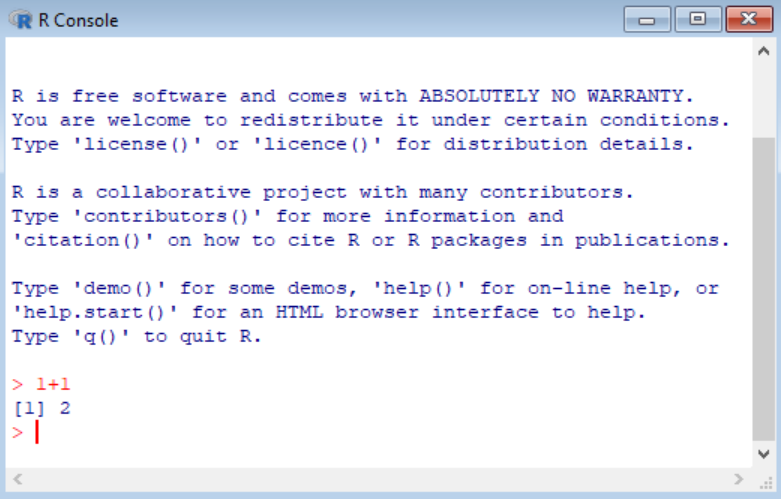
\includegraphics{images/arithmetic/arithmetic_console.png}

}

\caption{\label{fig-arithmetic-1}A basic arithmetic calculation in the R
Console}

\end{figure}%

Additionally, to include comments into the code block, we use the hash
(\texttt{\#}) symbol. Anything written after the code block will be
commented out and not run.

\begin{Shaded}
\begin{Highlighting}[]
\CommentTok{\# A simple arithmetic calculation (which is not run because of the hash symbol)}

\DecValTok{1} \SpecialCharTok{+} \DecValTok{1}
\end{Highlighting}
\end{Shaded}

\begin{verbatim}
[1] 2
\end{verbatim}

\subsection{Arithmetic operators}\label{arithmetic-operators}

Various arithmetic operators (listed below) can be used in R/RStudio.

\begin{longtable}[]{@{}cc@{}}
\toprule\noalign{}
Arithmetic Operator & Description \\
\midrule\noalign{}
\endhead
\bottomrule\noalign{}
\endlastfoot
\texttt{+} & Addition \\
\texttt{-} & Subtraction \\
\texttt{*} & Multiplication \\
\texttt{/} & Division \\
\texttt{**} or \texttt{\^{}} & Exponentiation \\
\texttt{\%\%} & Modulus (remainder after division) \\
\texttt{\%/\%} & Integer division \\
\end{longtable}

Example

Create an R script called ``my\_arithmetic\_1.R''

Run the following calculations in the script and save the file to the
working directory.

\subsubsection{Addition}\label{addition}

\begin{Shaded}
\begin{Highlighting}[]
\DecValTok{10} \SpecialCharTok{+} \DecValTok{30}
\end{Highlighting}
\end{Shaded}

\begin{verbatim}
[1] 40
\end{verbatim}

\subsubsection{Subtraction}\label{subtraction}

\begin{Shaded}
\begin{Highlighting}[]
\DecValTok{30} \SpecialCharTok{{-}} \DecValTok{24}
\end{Highlighting}
\end{Shaded}

\begin{verbatim}
[1] 6
\end{verbatim}

\subsubsection{Multiplication}\label{multiplication}

\begin{Shaded}
\begin{Highlighting}[]
\DecValTok{20} \SpecialCharTok{*} \DecValTok{4}
\end{Highlighting}
\end{Shaded}

\begin{verbatim}
[1] 80
\end{verbatim}

\subsubsection{Division}\label{division}

\begin{Shaded}
\begin{Highlighting}[]
\DecValTok{93} \SpecialCharTok{/} \DecValTok{4}
\end{Highlighting}
\end{Shaded}

\begin{verbatim}
[1] 23.25
\end{verbatim}

\subsubsection{Exponentiation}\label{exponentiation}

\begin{Shaded}
\begin{Highlighting}[]
\DecValTok{3}\SpecialCharTok{\^{}}\DecValTok{6}
\end{Highlighting}
\end{Shaded}

\begin{verbatim}
[1] 729
\end{verbatim}

\subsubsection{Modulus (remainder with
division)}\label{modulus-remainder-with-division}

\begin{Shaded}
\begin{Highlighting}[]
\DecValTok{94} \SpecialCharTok{\%\%} \DecValTok{5}
\end{Highlighting}
\end{Shaded}

\begin{verbatim}
[1] 4
\end{verbatim}

\subsubsection{Integer Division}\label{integer-division}

\begin{Shaded}
\begin{Highlighting}[]
\DecValTok{54} \SpecialCharTok{\%/\%} \DecValTok{7}
\end{Highlighting}
\end{Shaded}

\begin{verbatim}
[1] 7
\end{verbatim}

\subsubsection{Slightly more complex arithmetic
operations}\label{slightly-more-complex-arithmetic-operations}

\begin{Shaded}
\begin{Highlighting}[]
\DecValTok{5} \SpecialCharTok{{-}} \DecValTok{1} \SpecialCharTok{+}\NormalTok{ (}\DecValTok{4} \SpecialCharTok{*} \DecValTok{3}\NormalTok{) }\SpecialCharTok{/} \DecValTok{16} \SpecialCharTok{*} \DecValTok{3}
\end{Highlighting}
\end{Shaded}

\begin{verbatim}
[1] 6.25
\end{verbatim}

\subsection{Variables}\label{variables}

Variables are instrumental in programming because they are used as
``containers'' to store data values. To assign a value to a variable, we
can use \texttt{\textless{}−} or \texttt{=}. However, most R users
prefer to use \texttt{\textless{}−}.

\begin{itemize}
\tightlist
\item
  Variables store values for later use in your code. This results in
  improved readability and efficiency.
\item
  Assign values to variables using the \texttt{\textless{}-} operator
  (e.g., \texttt{x\ \textless{}-\ 5}).
\item
  Variable names should be descriptive and avoid special characters.
\end{itemize}

\subsubsection{Variable assignment}\label{variable-assignment}

\begin{enumerate}
\def\labelenumi{\arabic{enumi}.}
\tightlist
\item
  Using \texttt{\textless{}-}
\end{enumerate}

\begin{Shaded}
\begin{Highlighting}[]
\NormalTok{variable\_1 }\OtherTok{\textless{}{-}} \DecValTok{5}
\NormalTok{variable\_1}
\end{Highlighting}
\end{Shaded}

\begin{verbatim}
[1] 5
\end{verbatim}

\begin{enumerate}
\def\labelenumi{\arabic{enumi}.}
\setcounter{enumi}{1}
\tightlist
\item
  Using \texttt{=}
\end{enumerate}

\begin{Shaded}
\begin{Highlighting}[]
\NormalTok{variable\_2 }\OtherTok{\textless{}{-}} \DecValTok{10}
\NormalTok{variable\_2}
\end{Highlighting}
\end{Shaded}

\begin{verbatim}
[1] 10
\end{verbatim}

\begin{enumerate}
\def\labelenumi{\arabic{enumi}.}
\setcounter{enumi}{2}
\tightlist
\item
  Reverse the value and variable with \texttt{-\textgreater{}}
\end{enumerate}

\begin{Shaded}
\begin{Highlighting}[]
\DecValTok{15} \OtherTok{{-}\textgreater{}}\NormalTok{ variable\_3}
\NormalTok{variable\_3}
\end{Highlighting}
\end{Shaded}

\begin{verbatim}
[1] 15
\end{verbatim}

\begin{enumerate}
\def\labelenumi{\arabic{enumi}.}
\setcounter{enumi}{3}
\tightlist
\item
  Assign two variables to one value
\end{enumerate}

\begin{Shaded}
\begin{Highlighting}[]
\NormalTok{variable\_4 }\OtherTok{\textless{}{-}}\NormalTok{ variable\_5 }\OtherTok{\textless{}{-}} \DecValTok{30}
\NormalTok{variable\_4}
\end{Highlighting}
\end{Shaded}

\begin{verbatim}
[1] 30
\end{verbatim}

\begin{Shaded}
\begin{Highlighting}[]
\NormalTok{variable\_5}
\end{Highlighting}
\end{Shaded}

\begin{verbatim}
[1] 30
\end{verbatim}

The output of the variable can then be obtained by:

\begin{enumerate}
\def\labelenumi{\arabic{enumi}.}
\item
  Typing the variable name and then pressing ``Enter,''
\item
  Typing ``print'' with the variable name in brackets,
  \texttt{print(variable)}, and,
\item
  Typing ``View'' with the variable name in brackets,
  \texttt{View(variable)}.
\end{enumerate}

Both \texttt{print()} and \texttt{View()} are some of the many built-in
functions available in R.

\begin{figure}

\centering{

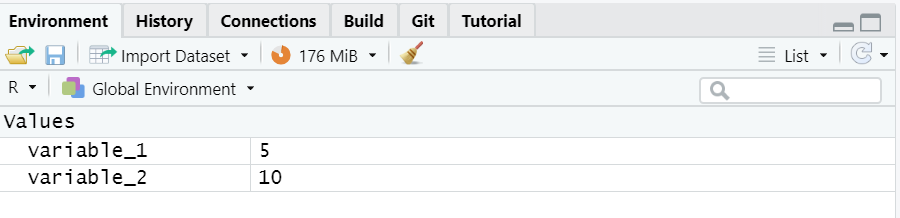
\includegraphics{images/arithmetic/environment_pane.png}

}

\caption{\label{fig-environment-1}The environment pane in RStudio with
stored variables}

\end{figure}%

\begin{Shaded}
\begin{Highlighting}[]
\FunctionTok{print}\NormalTok{(variable\_1)}
\end{Highlighting}
\end{Shaded}

\begin{verbatim}
[1] 5
\end{verbatim}

\begin{Shaded}
\begin{Highlighting}[]
\FunctionTok{View}\NormalTok{(variable\_2)}
\end{Highlighting}
\end{Shaded}

Output of \texttt{View()} will be seen in the script pane.

\subsubsection{\texorpdfstring{The \texttt{assign()} and \texttt{rm()}
functions}{The assign() and rm() functions}}\label{the-assign-and-rm-functions}

In addition to using the assignment operators (\texttt{\textless{}-} and
\texttt{=}), we can use the \texttt{assign()} function to assign a value
to a variable.

\begin{Shaded}
\begin{Highlighting}[]
\FunctionTok{assign}\NormalTok{(}\StringTok{"variable\_6"}\NormalTok{, }\DecValTok{555}\NormalTok{)}
\NormalTok{variable\_6}
\end{Highlighting}
\end{Shaded}

\begin{verbatim}
[1] 555
\end{verbatim}

To remove the assignment of the value to the variable, either delete the
variable in the ``environment pane'' or use the \texttt{rm()} function.

\begin{Shaded}
\begin{Highlighting}[]
\NormalTok{variable\_7 }\OtherTok{\textless{}{-}} \DecValTok{159}
\end{Highlighting}
\end{Shaded}

\begin{Shaded}
\begin{Highlighting}[]
\FunctionTok{rm}\NormalTok{(variable\_7)}
\end{Highlighting}
\end{Shaded}

After running \texttt{rm()} look at the environment pane to confirm
whether variable\_7 has been removed.

\subsubsection{Naming variables}\label{naming-variables}

At this point, you may be wondering what conventions are used for naming
variables. First, variables need to have meaningful names such as
current\_temp, time\_24\_hr, or weight\_lbs. However, we need to be
mindful of the variable style guide (link) which provides us with the
appropriate rules for naming variables.

\texttt{object\_name\ \textless{}-\ value}

Objects must start with a letter and only contain letters and numbers

Some rules to keep in mind are: 1. R is case-sensitive (variable is not
the same as Variable), 2. Names similar to typical outputs or functions
(TRUE, FALSE, if, or else) cannot be used, 3. Appropriate variable names
can contain letters, numbers, dots, and underscores. However, you cannot
start with an underscore, number, or dot followed by a number.

\subsubsection{Valid and invalid variable
names}\label{valid-and-invalid-variable-names}

Types of variable names:

\begin{itemize}
\tightlist
\item
  snake\_case
\item
  CamelCase
\item
  use.periods
\item
  snake.case.CamelCase\_snake\_case
\end{itemize}

Valid names:

\begin{itemize}
\item
  time\_24\_hr
\item
  .time24\_hr
\end{itemize}

Invalid names:

\begin{itemize}
\item
  \_24\_hr.time
\item
  24\_hr\_time
\item
  .24\_hr\_time
\end{itemize}

\section{Exercises}\label{exercises-5}

\begin{enumerate}
\def\labelenumi{\roman{enumi}.}
\tightlist
\item
  In R, calculate \texttt{3\ +\ 5} and then \texttt{4\ *\ 6}.
\item
  Assign the value 10 to a variable called x. Then calculate
  \texttt{x\ \^{}\ 2}. Next, calculate the expression
  \texttt{(3\ +\ x)\ *\ (x\ -\ 1)} using the x from before.
\item
  Declare a variable to store your age and assign a value to it. Print
  the variable value.
\item
  Create variables for the length and width of a rectangle and calculate
  its area.
\item
  Explain the rules for naming variables in R. Provide examples of valid
  and invalid variable names.
\item
  What is operator precedence in R? How does it work for arithmetic
  operators?
\item
  What data types can be used for arithmetic operations in R?
\item
  What is the difference between \texttt{\textless{}-} and \texttt{=}
  for assignment in R?
\end{enumerate}

\section{Summary}\label{summary-5}

In this chapter, I have demonstrated how to perform basic arithmetic
operations and how to use the various arithmetic operators available in
R/RStudio. Additionally, the concept of variables and values has been
explained, and conventions for appropriately naming variables have been
discussed. In the next chapter, we will look at the other types of
primary operators in R/RStudio.

\bookmarksetup{startatroot}

\chapter{The primary types of operators in R}\label{sec-operators}

\section{Questions}\label{questions-6}

\begin{itemize}
\item
  What are the primary operator types in R?
\item
  How can one use the various operator types in data analysis?
\item
  How do arithmetic, comparison, and logical operators work in R?
\item
  When should I use assignment operators versus comparison operators?
\end{itemize}

\section{Learning Objectives}\label{learning-objectives-6}

\begin{itemize}
\item
  Identify the primary operator types in R.
\item
  Learn how to use various operators for data manipulation.
\item
  Utilize arithmetic operators for efficient numerical calculations in
  your R scripts.
\item
  Apply comparison operators to evaluate conditions and filter data
  based on logical comparisons.
\item
  Employ logical operators to combine multiple conditions and control
  the flow of your R code.
\end{itemize}

\section{Lesson Content}\label{lesson-content-6}

\subsection{Introduction}\label{introduction-4}

R has many different types of operators that can perform different
tasks. Here we will focus on 5 major types of operators. The major types
of operators are:

\begin{itemize}
\tightlist
\item
  Arithmetic,
\item
  Relational,
\item
  Logical,
\item
  Assignment, and
\item
  Miscellaneous.
\end{itemize}

\subsection{Arithmetic Operators}\label{arithmetic-operators-1}

Arithmetic operators are used to perform mathematical operations. These
operators were reviewed in the previous lesson on ``Basic arithmetic,
arithmetic operators, and variables''
(Chapter~\ref{sec-arithmetic-variables})

\subsection{Relational Operators}\label{relational-operators}

Relational operators are used to find the relationship between 2
variables and compare objects. The output of these comparisons is
Boolean (TRUE or FALSE). The table below describes the most common
relational operators.

\begin{longtable}[]{@{}cc@{}}
\toprule\noalign{}
Relational Operator & Description \\
\midrule\noalign{}
\endhead
\bottomrule\noalign{}
\endlastfoot
\texttt{\textless{}} & Less than \\
\texttt{\textgreater{}} & Greater than \\
\texttt{\textless{}=} & Less than or equal to \\
\texttt{\textgreater{}=} & Greater than or equal to \\
\texttt{==} & Equal to \\
\texttt{!=} & Not Equal to \\
\end{longtable}

\subsubsection{Assign values to
variables}\label{assign-values-to-variables}

\begin{Shaded}
\begin{Highlighting}[]
\NormalTok{x }\OtherTok{\textless{}{-}} \DecValTok{227}
\NormalTok{y }\OtherTok{\textless{}{-}} \DecValTok{639}
\end{Highlighting}
\end{Shaded}

\begin{enumerate}
\def\labelenumi{\alph{enumi}.}
\tightlist
\item
  Less than
\end{enumerate}

\begin{Shaded}
\begin{Highlighting}[]
\NormalTok{x }\SpecialCharTok{\textless{}}\NormalTok{ y}
\end{Highlighting}
\end{Shaded}

\begin{verbatim}
[1] TRUE
\end{verbatim}

\begin{enumerate}
\def\labelenumi{\alph{enumi}.}
\setcounter{enumi}{1}
\tightlist
\item
  Greater than
\end{enumerate}

\begin{Shaded}
\begin{Highlighting}[]
\NormalTok{x }\SpecialCharTok{\textgreater{}}\NormalTok{ y}
\end{Highlighting}
\end{Shaded}

\begin{verbatim}
[1] FALSE
\end{verbatim}

\begin{enumerate}
\def\labelenumi{\alph{enumi}.}
\setcounter{enumi}{2}
\tightlist
\item
  Less than or equal to
\end{enumerate}

\begin{Shaded}
\begin{Highlighting}[]
\NormalTok{x }\SpecialCharTok{\textless{}=} \DecValTok{300}
\end{Highlighting}
\end{Shaded}

\begin{verbatim}
[1] TRUE
\end{verbatim}

\begin{enumerate}
\def\labelenumi{\alph{enumi}.}
\setcounter{enumi}{3}
\tightlist
\item
  Greater than or equal to
\end{enumerate}

\begin{Shaded}
\begin{Highlighting}[]
\NormalTok{y }\SpecialCharTok{\textgreater{}=} \DecValTok{700}
\end{Highlighting}
\end{Shaded}

\begin{verbatim}
[1] FALSE
\end{verbatim}

\begin{enumerate}
\def\labelenumi{\alph{enumi}.}
\setcounter{enumi}{4}
\tightlist
\item
  Equal to
\end{enumerate}

\begin{Shaded}
\begin{Highlighting}[]
\NormalTok{y }\SpecialCharTok{==} \DecValTok{639}
\end{Highlighting}
\end{Shaded}

\begin{verbatim}
[1] TRUE
\end{verbatim}

\begin{enumerate}
\def\labelenumi{\alph{enumi}.}
\setcounter{enumi}{5}
\tightlist
\item
  Not Equal to
\end{enumerate}

\begin{Shaded}
\begin{Highlighting}[]
\NormalTok{x }\SpecialCharTok{!=} \DecValTok{227}
\end{Highlighting}
\end{Shaded}

\begin{verbatim}
[1] FALSE
\end{verbatim}

\subsection{Logical Operators}\label{logical-operators}

Logical operators are used to specify multiple conditions between
objects. Logical operators work with basic data types such as logical,
numeric, and complex data types. This returns TRUE or FALSE values.
Numbers greater that 1 are TRUE and 0 equals FALSE. The table below
describes the most common logical operators.

\begin{longtable}[]{@{}cc@{}}
\toprule\noalign{}
Logical Operator & Description \\
\midrule\noalign{}
\endhead
\bottomrule\noalign{}
\endlastfoot
\texttt{!} & Logical NOT \\
\texttt{\textbar{}} & Element-wise logical OR \\
\texttt{\&} & Element-wise logical AND \\
\end{longtable}

\subsubsection{Assign vectors to
variables}\label{assign-vectors-to-variables}

NOTE: Full discussion in the chapter on ``Vectors''
(Chapter~\ref{sec-vectors})

\begin{Shaded}
\begin{Highlighting}[]
\NormalTok{vector\_1 }\OtherTok{\textless{}{-}} \FunctionTok{c}\NormalTok{(}\DecValTok{0}\NormalTok{,}\DecValTok{2}\NormalTok{)}
\NormalTok{vector\_2 }\OtherTok{\textless{}{-}} \FunctionTok{c}\NormalTok{(}\DecValTok{1}\NormalTok{,}\DecValTok{0}\NormalTok{)}
\end{Highlighting}
\end{Shaded}

\begin{enumerate}
\def\labelenumi{\alph{enumi}.}
\tightlist
\item
  Logical NOT
\end{enumerate}

\begin{Shaded}
\begin{Highlighting}[]
\SpecialCharTok{!}\NormalTok{vector\_1}
\end{Highlighting}
\end{Shaded}

\begin{verbatim}
[1]  TRUE FALSE
\end{verbatim}

\begin{Shaded}
\begin{Highlighting}[]
\SpecialCharTok{!}\NormalTok{vector\_2}
\end{Highlighting}
\end{Shaded}

\begin{verbatim}
[1] FALSE  TRUE
\end{verbatim}

\begin{enumerate}
\def\labelenumi{\alph{enumi}.}
\setcounter{enumi}{1}
\tightlist
\item
  Element-wise Logical OR
\end{enumerate}

\begin{Shaded}
\begin{Highlighting}[]
\NormalTok{vector\_1 }\SpecialCharTok{|}\NormalTok{ vector\_2}
\end{Highlighting}
\end{Shaded}

\begin{verbatim}
[1] TRUE TRUE
\end{verbatim}

\begin{enumerate}
\def\labelenumi{\alph{enumi}.}
\setcounter{enumi}{2}
\tightlist
\item
  Element-wise Logical AND
\end{enumerate}

\begin{Shaded}
\begin{Highlighting}[]
\NormalTok{vector\_1 }\SpecialCharTok{\&}\NormalTok{ vector\_2}
\end{Highlighting}
\end{Shaded}

\begin{verbatim}
[1] FALSE FALSE
\end{verbatim}

\subsection{Assignment Operators}\label{assignment-operators}

These operators assign values to variables. A more comprehensive review
can be obtained in the lesson on ``Basic arithmetic, arithmetic
operators, and variables'' (Chapter~\ref{sec-arithmetic-variables})

\subsection{Miscellaneous Operators}\label{miscellaneous-operators}

These are helpful operators for working in that can perform a variety of
functions. A few common miscellaneous operators are described below.

\begin{longtable}[]{@{}
  >{\centering\arraybackslash}p{(\columnwidth - 2\tabcolsep) * \real{0.2778}}
  >{\centering\arraybackslash}p{(\columnwidth - 2\tabcolsep) * \real{0.7222}}@{}}
\toprule\noalign{}
\begin{minipage}[b]{\linewidth}\centering
Miscellaneous Operator
\end{minipage} & \begin{minipage}[b]{\linewidth}\centering
Description
\end{minipage} \\
\midrule\noalign{}
\endhead
\bottomrule\noalign{}
\endlastfoot
\texttt{\%*\%} & Matrix multiplication (to be discussed in subsequent
chapters) \\
\texttt{\%in\%} & Does an element belong to a vector \\
\texttt{:} & Generate a sequence \\
\end{longtable}

\begin{enumerate}
\def\labelenumi{\alph{enumi}.}
\tightlist
\item
  Sequence
\end{enumerate}

\begin{Shaded}
\begin{Highlighting}[]
\NormalTok{a }\OtherTok{\textless{}{-}} \DecValTok{1}\SpecialCharTok{:}\DecValTok{8}
\NormalTok{a}
\end{Highlighting}
\end{Shaded}

\begin{verbatim}
[1] 1 2 3 4 5 6 7 8
\end{verbatim}

\begin{Shaded}
\begin{Highlighting}[]
\NormalTok{b }\OtherTok{\textless{}{-}} \DecValTok{4}\SpecialCharTok{:}\DecValTok{10}
\NormalTok{b}
\end{Highlighting}
\end{Shaded}

\begin{verbatim}
[1]  4  5  6  7  8  9 10
\end{verbatim}

\begin{enumerate}
\def\labelenumi{\alph{enumi}.}
\setcounter{enumi}{1}
\tightlist
\item
  Element in a vector
\end{enumerate}

\begin{Shaded}
\begin{Highlighting}[]
\NormalTok{a }\SpecialCharTok{\%in\%}\NormalTok{ b}
\end{Highlighting}
\end{Shaded}

\begin{verbatim}
[1] FALSE FALSE FALSE  TRUE  TRUE  TRUE  TRUE  TRUE
\end{verbatim}

\begin{Shaded}
\begin{Highlighting}[]
\DecValTok{9} \SpecialCharTok{\%in\%}\NormalTok{ b}
\end{Highlighting}
\end{Shaded}

\begin{verbatim}
[1] TRUE
\end{verbatim}

\begin{Shaded}
\begin{Highlighting}[]
\DecValTok{9} \SpecialCharTok{\%in\%}\NormalTok{ a}
\end{Highlighting}
\end{Shaded}

\begin{verbatim}
[1] FALSE
\end{verbatim}

\section{Exercises}\label{exercises-6}

\begin{itemize}
\item
  List the basic operator types in R and provide an example for each.
\item
  What operators allow you to subset vectors, lists, and data frames in
  R?
\item
  Explain how the modulus operator (\texttt{\%/\%}) differs from the
  regular division operator (\texttt{/}).
\item
  What are the membership operators \texttt{\%in\%} and \texttt{!\%in\%}
  used for in R?
\item
  Assign 10 to x using \texttt{\textless{}-}. Then compare if
  \texttt{x\ ==\ 10}.
\item
  Calculate \texttt{3\^{}4} using arithmetic operators.
\item
  Compare \texttt{3\ \textgreater{}\ 5}. Is the result TRUE or FALSE?
\item
  When would you use the sequence operator (\texttt{:}) in R? Give an
  example.
\end{itemize}

\section{Summary}\label{summary-6}

The focus of this chapter has been the five major types of operators
that can be used in R/RStudio. The operators allow one to perform
numerous tasks including basic arithmetic including basic arithmetic,
comparisons, subsetting, matrix multiplication, and vector generation.
In the next chapter, we will discuss the available data types in R and
how to utilize/handle them.

\bookmarksetup{startatroot}

\chapter{Data Types}\label{sec-data-types}

\section{Questions}\label{questions-7}

\begin{itemize}
\item
  What are the primary data types in R?
\item
  Can one convert between different data types?
\item
  How does R handle different types of data?
\item
  How can I determine the type of a variable in R?
\item
  What are some helpful functions for identifying and manipulating data
  types?
\item
  How do data types impact my analysis and coding in R?
\end{itemize}

\section{Learning Objectives}\label{learning-objectives-7}

\begin{itemize}
\item
  Identify and differentiate between common data types in R.
\item
  Learn how to convert between different data types.
\item
  Use functions like \texttt{class()}, \texttt{typeof()}, and
  \texttt{str()} to inspect types.
\item
  Convert between data types using the \texttt{as.\_\_\_()} functions.
\end{itemize}

\section{Lesson Content}\label{lesson-content-7}

\subsection{Introduction}\label{introduction-5}

R and RStudio utilize multiple data types to store different kinds of
data.

The most common data types in R are listed below.

\begin{longtable}[]{@{}
  >{\raggedright\arraybackslash}p{(\columnwidth - 2\tabcolsep) * \real{0.1806}}
  >{\raggedright\arraybackslash}p{(\columnwidth - 2\tabcolsep) * \real{0.8194}}@{}}
\toprule\noalign{}
\begin{minipage}[b]{\linewidth}\raggedright
\textbf{Data Type}
\end{minipage} & \begin{minipage}[b]{\linewidth}\raggedright
\textbf{Description}
\end{minipage} \\
\midrule\noalign{}
\endhead
\bottomrule\noalign{}
\endlastfoot
Numeric & The most common data type. The values can be numbers or
decimals (all real numbers). \\
Integer & Special case of numeric data without decimals. \\
Logical & Boolean data type with only 2 values (\texttt{TRUE} or
\texttt{FALSE}). \\
Complex & Specifies imaginary values in R. \\
Character & Assigns a character or string to a variable. The character
variables are enclosed in single quotes (`character') while the string
variables are enclosed in double quotes (``string''). \\
Factor & Special type of character variable that represents a
categorical such as gender. \\
Raw & Specifies values as raw bytes. It uses built-in functions to
convert between raw and character (\texttt{charToRaw()} or
\texttt{rawToChar()}). \\
Dates & Specifies the date variable. Date stores a date and POSIXct
stores a date and time. The output is indicated as the number of days
(Date) or number of seconds (POSIXct) since 01/01/1970. \\
\end{longtable}

\subsection{Examples of data types in
R}\label{examples-of-data-types-in-r}

\begin{enumerate}
\def\labelenumi{\arabic{enumi}.}
\tightlist
\item
  Numeric
\end{enumerate}

\begin{Shaded}
\begin{Highlighting}[]
\FloatTok{89.98}
\end{Highlighting}
\end{Shaded}

\begin{verbatim}
[1] 89.98
\end{verbatim}

\begin{Shaded}
\begin{Highlighting}[]
\DecValTok{55}
\end{Highlighting}
\end{Shaded}

\begin{verbatim}
[1] 55
\end{verbatim}

\begin{enumerate}
\def\labelenumi{\arabic{enumi}.}
\setcounter{enumi}{1}
\tightlist
\item
  Integer
\end{enumerate}

\begin{Shaded}
\begin{Highlighting}[]
\DecValTok{5}\NormalTok{L}
\end{Highlighting}
\end{Shaded}

\begin{verbatim}
[1] 5
\end{verbatim}

\begin{Shaded}
\begin{Highlighting}[]
\DecValTok{5768}\NormalTok{L}
\end{Highlighting}
\end{Shaded}

\begin{verbatim}
[1] 5768
\end{verbatim}

\begin{enumerate}
\def\labelenumi{\arabic{enumi}.}
\setcounter{enumi}{2}
\tightlist
\item
  Logical
\end{enumerate}

\begin{Shaded}
\begin{Highlighting}[]
\ConstantTok{TRUE}
\end{Highlighting}
\end{Shaded}

\begin{verbatim}
[1] TRUE
\end{verbatim}

\begin{Shaded}
\begin{Highlighting}[]
\ConstantTok{FALSE}
\end{Highlighting}
\end{Shaded}

\begin{verbatim}
[1] FALSE
\end{verbatim}

\begin{enumerate}
\def\labelenumi{\arabic{enumi}.}
\setcounter{enumi}{3}
\tightlist
\item
  Complex
\end{enumerate}

\begin{Shaded}
\begin{Highlighting}[]
\DecValTok{10} \SpecialCharTok{+} \DecValTok{30}\NormalTok{i}
\end{Highlighting}
\end{Shaded}

\begin{verbatim}
[1] 10+30i
\end{verbatim}

\begin{Shaded}
\begin{Highlighting}[]
\DecValTok{287} \SpecialCharTok{+} \DecValTok{34}\NormalTok{i}
\end{Highlighting}
\end{Shaded}

\begin{verbatim}
[1] 287+34i
\end{verbatim}

\begin{enumerate}
\def\labelenumi{\arabic{enumi}.}
\setcounter{enumi}{4}
\tightlist
\item
  Character or String
\end{enumerate}

\begin{Shaded}
\begin{Highlighting}[]
\StringTok{\textquotesingle{}abc\textquotesingle{}}
\end{Highlighting}
\end{Shaded}

\begin{verbatim}
[1] "abc"
\end{verbatim}

\begin{Shaded}
\begin{Highlighting}[]
\StringTok{"def"}
\end{Highlighting}
\end{Shaded}

\begin{verbatim}
[1] "def"
\end{verbatim}

\begin{Shaded}
\begin{Highlighting}[]
\StringTok{"I like learning R"}
\end{Highlighting}
\end{Shaded}

\begin{verbatim}
[1] "I like learning R"
\end{verbatim}

\textbf{NOTE: A comprehensive overview of handling characters with the
\texttt{stringr} package will be provided in a subsequent series on the
Tidyverse.}

\begin{enumerate}
\def\labelenumi{\arabic{enumi}.}
\setcounter{enumi}{5}
\tightlist
\item
  Dates
\end{enumerate}

\begin{Shaded}
\begin{Highlighting}[]
\StringTok{"2022{-}06{-}23 14:39:21 EAT"}
\end{Highlighting}
\end{Shaded}

\begin{verbatim}
[1] "2022-06-23 14:39:21 EAT"
\end{verbatim}

\begin{Shaded}
\begin{Highlighting}[]
\StringTok{"2022{-}06{-}23"}
\end{Highlighting}
\end{Shaded}

\begin{verbatim}
[1] "2022-06-23"
\end{verbatim}

\begin{enumerate}
\def\labelenumi{\arabic{enumi}.}
\setcounter{enumi}{6}
\tightlist
\item
  Raw
\end{enumerate}

\begin{enumerate}
\def\labelenumi{\arabic{enumi}.}
\setcounter{enumi}{7}
\tightlist
\item
  Factor
\end{enumerate}

\subsection{Inspecting various data
types}\label{inspecting-various-data-types}

Several functions exist to examine the features of the various data
types. These include:

1. \texttt{typeof()} -- what is the data type of the object (low-level)?

2. \texttt{class()} -- what is the data type of the object (high-level)?

3. \texttt{length()} -- how long is the object?

4. \texttt{attributes()} -- any metadata available?

Let's look at how these functions work with a few examples:

\begin{Shaded}
\begin{Highlighting}[]
\NormalTok{a }\OtherTok{\textless{}{-}} \FloatTok{45.84}
\NormalTok{b }\OtherTok{\textless{}{-}} \DecValTok{858}\NormalTok{L}
\NormalTok{c }\OtherTok{\textless{}{-}} \ConstantTok{TRUE}
\NormalTok{d }\OtherTok{\textless{}{-}} \DecValTok{89} \SpecialCharTok{+} \DecValTok{34}\NormalTok{i}
\NormalTok{e }\OtherTok{\textless{}{-}} \StringTok{\textquotesingle{}abc\textquotesingle{}}
\end{Highlighting}
\end{Shaded}

\begin{enumerate}
\def\labelenumi{\arabic{enumi}.}
\tightlist
\item
  Examine the data type at a low-level with \texttt{typeof()}
\end{enumerate}

\begin{Shaded}
\begin{Highlighting}[]
\FunctionTok{typeof}\NormalTok{(a)}
\end{Highlighting}
\end{Shaded}

\begin{verbatim}
[1] "double"
\end{verbatim}

\begin{Shaded}
\begin{Highlighting}[]
\FunctionTok{typeof}\NormalTok{(b)}
\end{Highlighting}
\end{Shaded}

\begin{verbatim}
[1] "integer"
\end{verbatim}

\begin{Shaded}
\begin{Highlighting}[]
\FunctionTok{typeof}\NormalTok{(c)}
\end{Highlighting}
\end{Shaded}

\begin{verbatim}
[1] "logical"
\end{verbatim}

\begin{Shaded}
\begin{Highlighting}[]
\FunctionTok{typeof}\NormalTok{(d)}
\end{Highlighting}
\end{Shaded}

\begin{verbatim}
[1] "complex"
\end{verbatim}

\begin{Shaded}
\begin{Highlighting}[]
\FunctionTok{typeof}\NormalTok{(e)}
\end{Highlighting}
\end{Shaded}

\begin{verbatim}
[1] "character"
\end{verbatim}

\begin{enumerate}
\def\labelenumi{\arabic{enumi}.}
\setcounter{enumi}{1}
\tightlist
\item
  Examine the data type at a high-level with \texttt{class()}
\end{enumerate}

\begin{Shaded}
\begin{Highlighting}[]
\FunctionTok{class}\NormalTok{(a)}
\end{Highlighting}
\end{Shaded}

\begin{verbatim}
[1] "numeric"
\end{verbatim}

\begin{Shaded}
\begin{Highlighting}[]
\FunctionTok{class}\NormalTok{(b)}
\end{Highlighting}
\end{Shaded}

\begin{verbatim}
[1] "integer"
\end{verbatim}

\begin{Shaded}
\begin{Highlighting}[]
\FunctionTok{class}\NormalTok{(c)}
\end{Highlighting}
\end{Shaded}

\begin{verbatim}
[1] "logical"
\end{verbatim}

\begin{Shaded}
\begin{Highlighting}[]
\FunctionTok{class}\NormalTok{(d)}
\end{Highlighting}
\end{Shaded}

\begin{verbatim}
[1] "complex"
\end{verbatim}

\begin{Shaded}
\begin{Highlighting}[]
\FunctionTok{class}\NormalTok{(e)}
\end{Highlighting}
\end{Shaded}

\begin{verbatim}
[1] "character"
\end{verbatim}

\begin{enumerate}
\def\labelenumi{\arabic{enumi}.}
\setcounter{enumi}{2}
\tightlist
\item
  Use the \texttt{is.\_\_\_\_()} functions to determine the data type.
  To test whether the variable is of a specific type, we can use the
  \texttt{is.\_\_\_\_()} functions.
\end{enumerate}

First, we test the variable a which is numeric.

\begin{Shaded}
\begin{Highlighting}[]
\FunctionTok{is.numeric}\NormalTok{(a)}
\end{Highlighting}
\end{Shaded}

\begin{verbatim}
[1] TRUE
\end{verbatim}

\begin{Shaded}
\begin{Highlighting}[]
\FunctionTok{is.integer}\NormalTok{(a)}
\end{Highlighting}
\end{Shaded}

\begin{verbatim}
[1] FALSE
\end{verbatim}

\begin{Shaded}
\begin{Highlighting}[]
\FunctionTok{is.logical}\NormalTok{(a)}
\end{Highlighting}
\end{Shaded}

\begin{verbatim}
[1] FALSE
\end{verbatim}

\begin{Shaded}
\begin{Highlighting}[]
\FunctionTok{is.character}\NormalTok{(a)}
\end{Highlighting}
\end{Shaded}

\begin{verbatim}
[1] FALSE
\end{verbatim}

Second, we test the variable c which is logical.

\begin{Shaded}
\begin{Highlighting}[]
\FunctionTok{is.numeric}\NormalTok{(c)}
\end{Highlighting}
\end{Shaded}

\begin{verbatim}
[1] FALSE
\end{verbatim}

\begin{Shaded}
\begin{Highlighting}[]
\FunctionTok{is.integer}\NormalTok{(c)}
\end{Highlighting}
\end{Shaded}

\begin{verbatim}
[1] FALSE
\end{verbatim}

\begin{Shaded}
\begin{Highlighting}[]
\FunctionTok{is.logical}\NormalTok{(c)}
\end{Highlighting}
\end{Shaded}

\begin{verbatim}
[1] TRUE
\end{verbatim}

\begin{Shaded}
\begin{Highlighting}[]
\FunctionTok{is.character}\NormalTok{(c)}
\end{Highlighting}
\end{Shaded}

\begin{verbatim}
[1] FALSE
\end{verbatim}

\subsection{Converting between various data
types}\label{converting-between-various-data-types}

To convert between data types we can use the \texttt{as.\_\_\_()}
functions. These include: \texttt{as.Date()}, \texttt{as.numeric()}, and
\texttt{as.factor()}. Additionally, other helpful functions include
\texttt{factor()} which adds levels to the data and \texttt{nchar()}
which provides the length of the data.

\subsubsection{Implicit vs Explicit
conversion}\label{implicit-vs-explicit-conversion}

Examples

\begin{Shaded}
\begin{Highlighting}[]
\FunctionTok{as.integer}\NormalTok{(a)}
\end{Highlighting}
\end{Shaded}

\begin{verbatim}
[1] 45
\end{verbatim}

\begin{Shaded}
\begin{Highlighting}[]
\FunctionTok{as.logical}\NormalTok{(}\DecValTok{0}\NormalTok{)}
\end{Highlighting}
\end{Shaded}

\begin{verbatim}
[1] FALSE
\end{verbatim}

\begin{Shaded}
\begin{Highlighting}[]
\FunctionTok{as.logical}\NormalTok{(}\DecValTok{1}\NormalTok{)}
\end{Highlighting}
\end{Shaded}

\begin{verbatim}
[1] TRUE
\end{verbatim}

\begin{Shaded}
\begin{Highlighting}[]
\FunctionTok{nchar}\NormalTok{(e)}
\end{Highlighting}
\end{Shaded}

\begin{verbatim}
[1] 3
\end{verbatim}

Order of precedence when converting between data types is:

Character \texttt{\textgreater{}} Numeric \texttt{\textgreater{}}
Integer \texttt{\textgreater{}} Logical

\section{Exercises}\label{exercises-7}

\begin{itemize}
\item
  What are the basic data types in R? Give examples of each.
\item
  How can you check the data type of a variable in R?
\item
  Use the \texttt{class()}, \texttt{typeof()}, and \texttt{str()}
  functions to check the data type of objects.
\item
  Describe the process of coercion in R.
\item
  Provide an example of implicit and explicit coercion between data
  types.
\item
  How can you coerce or convert between different data types in R?
\item
  What does it mean for an object in R to have attributes? What
  attributes are commonly used?
\end{itemize}

\section{Summary}\label{summary-7}

In this chapter, I have demonstrated the primary data types in R.
Additionally, the learner has been trained on how to identify and
convert between the different data types. Next, we will review vectors,
which are key data structures in R/RStudio.

\bookmarksetup{startatroot}

\chapter{Vectors}\label{sec-vectors}

\section{Questions}\label{questions-8}

\begin{itemize}
\item
  What are vectors and why are they essential in R?
\item
  What are the different types of vectors and their key characteristics?
\item
  How does one create a vector?
\item
  What operations can be performed on a vector?
\item
  How do I create and access different elements within a vector?
\item
  Can I combine and manipulate vectors to achieve specific tasks?
\item
  What are some common functions for working with vectors?
\end{itemize}

\section{Learning Objectives}\label{learning-objectives-8}

\begin{itemize}
\item
  Define and create vectors in R.
\item
  Understand how to perform basic operations on vectors.
\item
  Understand the concept of vectors as fundamental data structures in R.
\item
  Master the creation and manipulation of vectors using various
  techniques.
\item
  Identify and differentiate between different types of vectors based on
  their elements.
\item
  Utilize functions and operators to combine, subset, and transform
  vectors with ease.
\item
  Apply your understanding of vectors to enhance your R coding and data
  analysis efficiency.
\end{itemize}

\section{Lesson Content}\label{lesson-content-8}

\subsection{Introduction}\label{introduction-6}

A vector is a collection of elements of the same data type, and they are
a basic data structure in R programming.

Vectors cannot be of mixed data type. The most common way to create a
vector is with \texttt{c()}, where ``c'' stands for combine. In R,
vectors do not have dimensions; therefore, they cannot be defined by
columns or rows. Vectors can be divided into atomic vectors and lists
(discussed in the ``Data Structures''
\{Chapter~\ref{sec-data-structure-1}\} section). The atomic vectors
include logical, character, and numeric (integer or double).

Additionally, R is a vectorized language because mathematical operations
are applied to each element of the vector without the need to loop
through the vector.

Examples of vectors made up of different data types are shown below:

\begin{itemize}
\tightlist
\item
  Numbers
\end{itemize}

\begin{Shaded}
\begin{Highlighting}[]
\FunctionTok{c}\NormalTok{(}\DecValTok{2}\NormalTok{, }\DecValTok{10}\NormalTok{, }\DecValTok{16}\NormalTok{, }\SpecialCharTok{{-}}\DecValTok{5}\NormalTok{)}
\end{Highlighting}
\end{Shaded}

\begin{verbatim}
[1]  2 10 16 -5
\end{verbatim}

\begin{itemize}
\tightlist
\item
  Characters
\end{itemize}

\begin{Shaded}
\begin{Highlighting}[]
\FunctionTok{c}\NormalTok{(}\StringTok{"R"}\NormalTok{, }\StringTok{"RStudio"}\NormalTok{, }\StringTok{"Shiny"}\NormalTok{, }\StringTok{"Quarto"}\NormalTok{)}
\end{Highlighting}
\end{Shaded}

\begin{verbatim}
[1] "R"       "RStudio" "Shiny"   "Quarto" 
\end{verbatim}

\begin{itemize}
\tightlist
\item
  Logicals
\end{itemize}

\begin{Shaded}
\begin{Highlighting}[]
\FunctionTok{c}\NormalTok{(}\StringTok{"TRUE"}\NormalTok{, }\StringTok{"FALSE"}\NormalTok{, }\StringTok{"TRUE"}\NormalTok{)}
\end{Highlighting}
\end{Shaded}

\begin{verbatim}
[1] "TRUE"  "FALSE" "TRUE" 
\end{verbatim}

\subsection{Sequence Generation}\label{sequence-generation}

To generate a vector with a sequence of consecutive numbers, we can use:
\texttt{sequence()}, or \texttt{seq()}.

Generate a sequence using \texttt{:}

\begin{Shaded}
\begin{Highlighting}[]
\NormalTok{a }\OtherTok{\textless{}{-}} \DecValTok{9}\SpecialCharTok{:}\DecValTok{18}
\NormalTok{a}
\end{Highlighting}
\end{Shaded}

\begin{verbatim}
 [1]  9 10 11 12 13 14 15 16 17 18
\end{verbatim}

\begin{Shaded}
\begin{Highlighting}[]
\NormalTok{a\_rev }\OtherTok{\textless{}{-}} \DecValTok{18}\SpecialCharTok{:}\DecValTok{9}
\NormalTok{a\_rev}
\end{Highlighting}
\end{Shaded}

\begin{verbatim}
 [1] 18 17 16 15 14 13 12 11 10  9
\end{verbatim}

\begin{Shaded}
\begin{Highlighting}[]
\NormalTok{a\_rev\_minus }\OtherTok{\textless{}{-}} \DecValTok{5}\SpecialCharTok{:{-}}\DecValTok{3}
\NormalTok{a\_rev\_minus}
\end{Highlighting}
\end{Shaded}

\begin{verbatim}
[1]  5  4  3  2  1  0 -1 -2 -3
\end{verbatim}

Generate a sequence using \texttt{sequence()}

\begin{Shaded}
\begin{Highlighting}[]
\NormalTok{b }\OtherTok{\textless{}{-}} \FunctionTok{sequence}\NormalTok{(}\DecValTok{7}\NormalTok{)}
\NormalTok{b}
\end{Highlighting}
\end{Shaded}

\begin{verbatim}
[1] 1 2 3 4 5 6 7
\end{verbatim}

\begin{Shaded}
\begin{Highlighting}[]
\NormalTok{c }\OtherTok{\textless{}{-}} \FunctionTok{sequence}\NormalTok{(}\FunctionTok{c}\NormalTok{(}\DecValTok{5}\NormalTok{,}\DecValTok{9}\NormalTok{))}
\NormalTok{c}
\end{Highlighting}
\end{Shaded}

\begin{verbatim}
 [1] 1 2 3 4 5 1 2 3 4 5 6 7 8 9
\end{verbatim}

Generate a sequence using \texttt{seq()}

The \texttt{seq()} function has four main arguments:
\texttt{seq(from,\ to,\ by,\ length.out)}, where ``from'' and ``to'' are
the starting and ending elements of the sequence. Additionally, ``by''
is the difference between the elements, and ``length.out'' is the
maximum length of the vector.

\begin{Shaded}
\begin{Highlighting}[]
\NormalTok{d }\OtherTok{\textless{}{-}} \FunctionTok{seq}\NormalTok{(}\DecValTok{2}\NormalTok{,}\DecValTok{20}\NormalTok{,}\AttributeTok{by=}\DecValTok{2}\NormalTok{)}
\NormalTok{d}
\end{Highlighting}
\end{Shaded}

\begin{verbatim}
 [1]  2  4  6  8 10 12 14 16 18 20
\end{verbatim}

\begin{Shaded}
\begin{Highlighting}[]
\NormalTok{f }\OtherTok{\textless{}{-}} \FunctionTok{seq}\NormalTok{(}\DecValTok{2}\NormalTok{,}\DecValTok{20}\NormalTok{, }\AttributeTok{length.out=}\DecValTok{5}\NormalTok{)}
\NormalTok{f}
\end{Highlighting}
\end{Shaded}

\begin{verbatim}
[1]  2.0  6.5 11.0 15.5 20.0
\end{verbatim}

\begin{Shaded}
\begin{Highlighting}[]
\NormalTok{h }\OtherTok{\textless{}{-}} \FunctionTok{seq}\NormalTok{(}\DecValTok{20}\NormalTok{,}\DecValTok{2}\NormalTok{,}\AttributeTok{by=}\SpecialCharTok{{-}}\DecValTok{2}\NormalTok{)}
\NormalTok{h}
\end{Highlighting}
\end{Shaded}

\begin{verbatim}
 [1] 20 18 16 14 12 10  8  6  4  2
\end{verbatim}

\begin{Shaded}
\begin{Highlighting}[]
\NormalTok{j }\OtherTok{\textless{}{-}} \FunctionTok{seq}\NormalTok{(}\DecValTok{20}\NormalTok{, }\DecValTok{2}\NormalTok{, }\AttributeTok{length.out=}\DecValTok{3}\NormalTok{)}
\NormalTok{j}
\end{Highlighting}
\end{Shaded}

\begin{verbatim}
[1] 20 11  2
\end{verbatim}

The \texttt{seq()} function can also be used with the arguments first,
by, and length.

\texttt{seq(first,\ by\ =\ \_\_\_,\ length\ =\ \_\_\_\_)}

Example

\begin{Shaded}
\begin{Highlighting}[]
\FunctionTok{seq}\NormalTok{(}\DecValTok{3}\NormalTok{, }\AttributeTok{by =} \DecValTok{4}\NormalTok{, }\AttributeTok{length =} \DecValTok{30}\NormalTok{)}
\end{Highlighting}
\end{Shaded}

\begin{verbatim}
 [1]   3   7  11  15  19  23  27  31  35  39  43  47  51  55  59  63  67  71  75
[20]  79  83  87  91  95  99 103 107 111 115 119
\end{verbatim}

Repeating vectors

To create a repeating vector, we can use \texttt{rep()}.

\texttt{rep(number,\ times)}

\begin{Shaded}
\begin{Highlighting}[]
\NormalTok{k }\OtherTok{\textless{}{-}} \FunctionTok{rep}\NormalTok{(}\FunctionTok{c}\NormalTok{(}\DecValTok{0}\NormalTok{,}\DecValTok{3}\NormalTok{,}\DecValTok{6}\NormalTok{), }\AttributeTok{times =} \DecValTok{3}\NormalTok{)}
\NormalTok{k}
\end{Highlighting}
\end{Shaded}

\begin{verbatim}
[1] 0 3 6 0 3 6 0 3 6
\end{verbatim}

\texttt{rep(range,\ times)}

\begin{Shaded}
\begin{Highlighting}[]
\NormalTok{l }\OtherTok{\textless{}{-}} \FunctionTok{rep}\NormalTok{(}\DecValTok{2}\SpecialCharTok{:}\DecValTok{6}\NormalTok{, }\AttributeTok{each =} \DecValTok{3}\NormalTok{)}
\NormalTok{l}
\end{Highlighting}
\end{Shaded}

\begin{verbatim}
 [1] 2 2 2 3 3 3 4 4 4 5 5 5 6 6 6
\end{verbatim}

\texttt{rep(number\ or\ range,\ length.out)}

\begin{Shaded}
\begin{Highlighting}[]
\NormalTok{m }\OtherTok{\textless{}{-}} \FunctionTok{rep}\NormalTok{(}\DecValTok{7}\NormalTok{, }\AttributeTok{length.out =} \DecValTok{20}\NormalTok{)}
\NormalTok{m}
\end{Highlighting}
\end{Shaded}

\begin{verbatim}
 [1] 7 7 7 7 7 7 7 7 7 7 7 7 7 7 7 7 7 7 7 7
\end{verbatim}

\begin{Shaded}
\begin{Highlighting}[]
\NormalTok{n }\OtherTok{\textless{}{-}} \FunctionTok{rep}\NormalTok{(}\DecValTok{7}\SpecialCharTok{:}\DecValTok{10}\NormalTok{, }\AttributeTok{length.out =} \DecValTok{20}\NormalTok{)}
\NormalTok{n}
\end{Highlighting}
\end{Shaded}

\begin{verbatim}
 [1]  7  8  9 10  7  8  9 10  7  8  9 10  7  8  9 10  7  8  9 10
\end{verbatim}

Random number generation

The \texttt{runif()} function can be used to generate a specific number
of random numbers between a minimum and maximum value.

\texttt{runif(n,\ min\ =\ 0,\ max\ =\ 1)}

\begin{Shaded}
\begin{Highlighting}[]
\FunctionTok{runif}\NormalTok{(}\DecValTok{5}\NormalTok{, }\AttributeTok{min =} \DecValTok{3}\NormalTok{, }\AttributeTok{max =} \DecValTok{100}\NormalTok{)}
\end{Highlighting}
\end{Shaded}

\begin{verbatim}
[1] 59.94056 75.51165 13.48448 88.33481 10.15589
\end{verbatim}

\textbf{NOTE} If you run the previous code block multiple times you will
get different answers. Use \texttt{set.seed()} to get a similar sequence
every time you run the calculation.

\begin{Shaded}
\begin{Highlighting}[]
\FunctionTok{set.seed}\NormalTok{(}\DecValTok{12345}\NormalTok{)}
\FunctionTok{runif}\NormalTok{(}\DecValTok{5}\NormalTok{, }\AttributeTok{min =} \DecValTok{3}\NormalTok{, }\AttributeTok{max =} \DecValTok{100}\NormalTok{)}
\end{Highlighting}
\end{Shaded}

\begin{verbatim}
[1] 72.92768 87.95000 76.81529 88.95408 47.27865
\end{verbatim}

\subsection{More functions to manipulate
vectors}\label{more-functions-to-manipulate-vectors}

Generate a random vector with 50 elements

\begin{Shaded}
\begin{Highlighting}[]
\FunctionTok{set.seed}\NormalTok{(}\DecValTok{54321}\NormalTok{)}
\NormalTok{sam }\OtherTok{\textless{}{-}} \FunctionTok{runif}\NormalTok{(}\DecValTok{50}\NormalTok{, }\AttributeTok{min =} \DecValTok{3}\NormalTok{, }\AttributeTok{max =} \DecValTok{100}\NormalTok{)}
\NormalTok{sam}
\end{Highlighting}
\end{Shaded}

\begin{verbatim}
 [1] 44.613758 51.347751 20.139157 29.616173 24.001486 87.037027  7.792779
 [8] 23.286089 36.136404 39.050902 16.254312 68.576625  7.394091 66.313937
[15] 99.424403 68.730823 92.098882 47.857159 58.427236 46.838066 19.267580
[22]  9.621351 90.000337 29.562192 93.228959 55.463536 70.832691 83.908744
[29]  4.192446 96.148363 69.028603 11.220652 97.050041 14.255861 88.055533
[36] 40.604467 91.237585 75.716659 87.464208 58.556042 90.634738 22.596315
[43] 69.616442 42.760092 94.441217 59.342340 63.392800 88.172536 12.631948
[50] 94.952417
\end{verbatim}

Sample

\begin{Shaded}
\begin{Highlighting}[]
\FunctionTok{sample}\NormalTok{(sam, }\AttributeTok{size =} \DecValTok{15}\NormalTok{)}
\end{Highlighting}
\end{Shaded}

\begin{verbatim}
 [1] 22.596315 91.237585 66.313937 68.576625 14.255861  9.621351 63.392800
 [8] 47.857159 55.463536 11.220652 36.136404 70.832691 93.228959  7.394091
[15] 83.908744
\end{verbatim}

To get the same sample repeatedly

\begin{Shaded}
\begin{Highlighting}[]
\FunctionTok{set.seed}\NormalTok{(}\DecValTok{1234}\NormalTok{)}
\FunctionTok{sample}\NormalTok{(sam, }\AttributeTok{size =} \DecValTok{15}\NormalTok{)}
\end{Highlighting}
\end{Shaded}

\begin{verbatim}
 [1] 83.908744 68.730823  9.621351 91.237585 42.760092 36.136404 24.001486
 [8] 75.716659 12.631948 29.616173 14.255861 87.464208 88.172536 55.463536
[15] 87.037027
\end{verbatim}

\begin{Shaded}
\begin{Highlighting}[]
\FunctionTok{sort}\NormalTok{(sam)}
\end{Highlighting}
\end{Shaded}

\begin{verbatim}
 [1]  4.192446  7.394091  7.792779  9.621351 11.220652 12.631948 14.255861
 [8] 16.254312 19.267580 20.139157 22.596315 23.286089 24.001486 29.562192
[15] 29.616173 36.136404 39.050902 40.604467 42.760092 44.613758 46.838066
[22] 47.857159 51.347751 55.463536 58.427236 58.556042 59.342340 63.392800
[29] 66.313937 68.576625 68.730823 69.028603 69.616442 70.832691 75.716659
[36] 83.908744 87.037027 87.464208 88.055533 88.172536 90.000337 90.634738
[43] 91.237585 92.098882 93.228959 94.441217 94.952417 96.148363 97.050041
[50] 99.424403
\end{verbatim}

\begin{Shaded}
\begin{Highlighting}[]
\FunctionTok{rev}\NormalTok{(}\FunctionTok{sort}\NormalTok{(sam))}
\end{Highlighting}
\end{Shaded}

\begin{verbatim}
 [1] 99.424403 97.050041 96.148363 94.952417 94.441217 93.228959 92.098882
 [8] 91.237585 90.634738 90.000337 88.172536 88.055533 87.464208 87.037027
[15] 83.908744 75.716659 70.832691 69.616442 69.028603 68.730823 68.576625
[22] 66.313937 63.392800 59.342340 58.556042 58.427236 55.463536 51.347751
[29] 47.857159 46.838066 44.613758 42.760092 40.604467 39.050902 36.136404
[36] 29.616173 29.562192 24.001486 23.286089 22.596315 20.139157 19.267580
[43] 16.254312 14.255861 12.631948 11.220652  9.621351  7.792779  7.394091
[50]  4.192446
\end{verbatim}

\begin{Shaded}
\begin{Highlighting}[]
\FunctionTok{quantile}\NormalTok{(sam)}
\end{Highlighting}
\end{Shaded}

\begin{verbatim}
       0%       25%       50%       75%      100% 
 4.192446 25.391662 58.491639 87.357413 99.424403 
\end{verbatim}

Create two vectors and look at the similarities/differences between the
two

\begin{Shaded}
\begin{Highlighting}[]
\FunctionTok{set.seed}\NormalTok{(}\DecValTok{2468}\NormalTok{)}
\NormalTok{vec\_top\_1 }\OtherTok{\textless{}{-}} \FunctionTok{seq}\NormalTok{(}\DecValTok{2}\NormalTok{, }\AttributeTok{by =} \DecValTok{6}\NormalTok{, }\AttributeTok{length =} \DecValTok{100}\NormalTok{)}
\NormalTok{vec\_top\_2 }\OtherTok{\textless{}{-}} \FunctionTok{seq}\NormalTok{(}\DecValTok{4}\NormalTok{, }\AttributeTok{by =} \DecValTok{4}\NormalTok{, }\AttributeTok{length =} \DecValTok{100}\NormalTok{)}
\end{Highlighting}
\end{Shaded}

\begin{Shaded}
\begin{Highlighting}[]
\NormalTok{vec\_top\_1 }
\end{Highlighting}
\end{Shaded}

\begin{verbatim}
  [1]   2   8  14  20  26  32  38  44  50  56  62  68  74  80  86  92  98 104
 [19] 110 116 122 128 134 140 146 152 158 164 170 176 182 188 194 200 206 212
 [37] 218 224 230 236 242 248 254 260 266 272 278 284 290 296 302 308 314 320
 [55] 326 332 338 344 350 356 362 368 374 380 386 392 398 404 410 416 422 428
 [73] 434 440 446 452 458 464 470 476 482 488 494 500 506 512 518 524 530 536
 [91] 542 548 554 560 566 572 578 584 590 596
\end{verbatim}

\begin{Shaded}
\begin{Highlighting}[]
\NormalTok{vec\_top\_2}
\end{Highlighting}
\end{Shaded}

\begin{verbatim}
  [1]   4   8  12  16  20  24  28  32  36  40  44  48  52  56  60  64  68  72
 [19]  76  80  84  88  92  96 100 104 108 112 116 120 124 128 132 136 140 144
 [37] 148 152 156 160 164 168 172 176 180 184 188 192 196 200 204 208 212 216
 [55] 220 224 228 232 236 240 244 248 252 256 260 264 268 272 276 280 284 288
 [73] 292 296 300 304 308 312 316 320 324 328 332 336 340 344 348 352 356 360
 [91] 364 368 372 376 380 384 388 392 396 400
\end{verbatim}

\begin{Shaded}
\begin{Highlighting}[]
\FunctionTok{union}\NormalTok{(vec\_top\_1, vec\_top\_2)}
\end{Highlighting}
\end{Shaded}

\begin{verbatim}
  [1]   2   8  14  20  26  32  38  44  50  56  62  68  74  80  86  92  98 104
 [19] 110 116 122 128 134 140 146 152 158 164 170 176 182 188 194 200 206 212
 [37] 218 224 230 236 242 248 254 260 266 272 278 284 290 296 302 308 314 320
 [55] 326 332 338 344 350 356 362 368 374 380 386 392 398 404 410 416 422 428
 [73] 434 440 446 452 458 464 470 476 482 488 494 500 506 512 518 524 530 536
 [91] 542 548 554 560 566 572 578 584 590 596   4  12  16  24  28  36  40  48
[109]  52  60  64  72  76  84  88  96 100 108 112 120 124 132 136 144 148 156
[127] 160 168 172 180 184 192 196 204 208 216 220 228 232 240 244 252 256 264
[145] 268 276 280 288 292 300 304 312 316 324 328 336 340 348 352 360 364 372
[163] 376 384 388 396 400
\end{verbatim}

\begin{Shaded}
\begin{Highlighting}[]
\FunctionTok{intersect}\NormalTok{(vec\_top\_1, vec\_top\_2)}
\end{Highlighting}
\end{Shaded}

\begin{verbatim}
 [1]   8  20  32  44  56  68  80  92 104 116 128 140 152 164 176 188 200 212 224
[20] 236 248 260 272 284 296 308 320 332 344 356 368 380 392
\end{verbatim}

\begin{Shaded}
\begin{Highlighting}[]
\FunctionTok{setdiff}\NormalTok{(vec\_top\_1, vec\_top\_2)}
\end{Highlighting}
\end{Shaded}

\begin{verbatim}
 [1]   2  14  26  38  50  62  74  86  98 110 122 134 146 158 170 182 194 206 218
[20] 230 242 254 266 278 290 302 314 326 338 350 362 374 386 398 404 410 416 422
[39] 428 434 440 446 452 458 464 470 476 482 488 494 500 506 512 518 524 530 536
[58] 542 548 554 560 566 572 578 584 590 596
\end{verbatim}

\subsection{Vector Operations}\label{vector-operations}

Vectors of equal length can be operated on together. If one vector is
shorter, it will get recycled, as its elements are repeated until it
matches the elements of the longer vector. When using vectors of unequal
lengths, it would be ideal if the longer vector is a multiple of the
shorter vector.

\begin{enumerate}
\def\labelenumi{\arabic{enumi}.}
\tightlist
\item
  Basic Vector Operations
\end{enumerate}

\begin{Shaded}
\begin{Highlighting}[]
\NormalTok{vec\_1 }\OtherTok{\textless{}{-}} \DecValTok{1}\SpecialCharTok{:}\DecValTok{10}
\end{Highlighting}
\end{Shaded}

\begin{Shaded}
\begin{Highlighting}[]
\NormalTok{vec\_1 }\SpecialCharTok{*} \DecValTok{12} \CommentTok{\# multiplication}
\end{Highlighting}
\end{Shaded}

\begin{verbatim}
 [1]  12  24  36  48  60  72  84  96 108 120
\end{verbatim}

\begin{Shaded}
\begin{Highlighting}[]
\NormalTok{vec\_1 }\SpecialCharTok{+} \DecValTok{12} \CommentTok{\# addition}
\end{Highlighting}
\end{Shaded}

\begin{verbatim}
 [1] 13 14 15 16 17 18 19 20 21 22
\end{verbatim}

\begin{Shaded}
\begin{Highlighting}[]
\NormalTok{vec\_1 }\SpecialCharTok{{-}} \DecValTok{12} \CommentTok{\# subtraction}
\end{Highlighting}
\end{Shaded}

\begin{verbatim}
 [1] -11 -10  -9  -8  -7  -6  -5  -4  -3  -2
\end{verbatim}

\begin{Shaded}
\begin{Highlighting}[]
\NormalTok{vec\_1 }\SpecialCharTok{/} \DecValTok{3} \CommentTok{\# division}
\end{Highlighting}
\end{Shaded}

\begin{verbatim}
 [1] 0.3333333 0.6666667 1.0000000 1.3333333 1.6666667 2.0000000 2.3333333
 [8] 2.6666667 3.0000000 3.3333333
\end{verbatim}

\begin{Shaded}
\begin{Highlighting}[]
\NormalTok{vec\_1}\SpecialCharTok{\^{}}\DecValTok{4} \CommentTok{\# power}
\end{Highlighting}
\end{Shaded}

\begin{verbatim}
 [1]     1    16    81   256   625  1296  2401  4096  6561 10000
\end{verbatim}

\begin{Shaded}
\begin{Highlighting}[]
\FunctionTok{sqrt}\NormalTok{(vec\_1) }\CommentTok{\# square root}
\end{Highlighting}
\end{Shaded}

\begin{verbatim}
 [1] 1.000000 1.414214 1.732051 2.000000 2.236068 2.449490 2.645751 2.828427
 [9] 3.000000 3.162278
\end{verbatim}

\begin{enumerate}
\def\labelenumi{\arabic{enumi}.}
\setcounter{enumi}{1}
\tightlist
\item
  Operations on vectors
\end{enumerate}

Operations on vectors of equal length Additionally, we can perform
operations on two vectors of equal length.

\begin{enumerate}
\def\labelenumi{\alph{enumi}.}
\tightlist
\item
  Create two vectors
\end{enumerate}

\begin{Shaded}
\begin{Highlighting}[]
\NormalTok{vec\_3 }\OtherTok{\textless{}{-}} \DecValTok{5}\SpecialCharTok{:}\DecValTok{14}
\NormalTok{vec\_3}
\end{Highlighting}
\end{Shaded}

\begin{verbatim}
 [1]  5  6  7  8  9 10 11 12 13 14
\end{verbatim}

\begin{Shaded}
\begin{Highlighting}[]
\NormalTok{vec\_4 }\OtherTok{\textless{}{-}} \DecValTok{12}\SpecialCharTok{:}\DecValTok{3}
\NormalTok{vec\_4}
\end{Highlighting}
\end{Shaded}

\begin{verbatim}
 [1] 12 11 10  9  8  7  6  5  4  3
\end{verbatim}

\begin{enumerate}
\def\labelenumi{\alph{enumi}.}
\setcounter{enumi}{1}
\tightlist
\item
  Perform various arithmetic operations
\end{enumerate}

\begin{Shaded}
\begin{Highlighting}[]
\NormalTok{vec\_3 }\SpecialCharTok{+}\NormalTok{ vec\_4}
\end{Highlighting}
\end{Shaded}

\begin{verbatim}
 [1] 17 17 17 17 17 17 17 17 17 17
\end{verbatim}

\begin{Shaded}
\begin{Highlighting}[]
\NormalTok{vec\_3 }\SpecialCharTok{{-}}\NormalTok{ vec\_4}
\end{Highlighting}
\end{Shaded}

\begin{verbatim}
 [1] -7 -5 -3 -1  1  3  5  7  9 11
\end{verbatim}

\begin{Shaded}
\begin{Highlighting}[]
\NormalTok{vec\_3 }\SpecialCharTok{/}\NormalTok{ vec\_4}
\end{Highlighting}
\end{Shaded}

\begin{verbatim}
 [1] 0.4166667 0.5454545 0.7000000 0.8888889 1.1250000 1.4285714 1.8333333
 [8] 2.4000000 3.2500000 4.6666667
\end{verbatim}

\begin{Shaded}
\begin{Highlighting}[]
\NormalTok{vec\_3 }\SpecialCharTok{*}\NormalTok{ vec\_4}
\end{Highlighting}
\end{Shaded}

\begin{verbatim}
 [1] 60 66 70 72 72 70 66 60 52 42
\end{verbatim}

\begin{Shaded}
\begin{Highlighting}[]
\NormalTok{vec\_3 }\SpecialCharTok{\^{}}\NormalTok{ vec\_4}
\end{Highlighting}
\end{Shaded}

\begin{verbatim}
 [1] 244140625 362797056 282475249 134217728  43046721  10000000   1771561
 [8]    248832     28561      2744
\end{verbatim}

\begin{enumerate}
\def\labelenumi{\arabic{enumi}.}
\setcounter{enumi}{2}
\tightlist
\item
  Functions that can be applied to vectors
\end{enumerate}

The functions listed below can be applied to vectors:

\begin{enumerate}
\def\labelenumi{\alph{enumi}.}
\item
  \texttt{any()}
\item
  \texttt{all()}
\item
  \texttt{nchar()}
\item
  \texttt{length()}
\item
  \texttt{typeof()}
\end{enumerate}

Examples

\begin{Shaded}
\begin{Highlighting}[]
\FunctionTok{any}\NormalTok{(vec\_3 }\SpecialCharTok{\textgreater{}}\NormalTok{ vec\_4)}
\end{Highlighting}
\end{Shaded}

\begin{verbatim}
[1] TRUE
\end{verbatim}

\begin{Shaded}
\begin{Highlighting}[]
\FunctionTok{any}\NormalTok{(vec\_3 }\SpecialCharTok{\textless{}}\NormalTok{ vec\_4)}
\end{Highlighting}
\end{Shaded}

\begin{verbatim}
[1] TRUE
\end{verbatim}

\begin{Shaded}
\begin{Highlighting}[]
\FunctionTok{all}\NormalTok{(vec\_3 }\SpecialCharTok{\textgreater{}}\NormalTok{ vec\_4)}
\end{Highlighting}
\end{Shaded}

\begin{verbatim}
[1] FALSE
\end{verbatim}

\begin{Shaded}
\begin{Highlighting}[]
\FunctionTok{all}\NormalTok{(vec\_3 }\SpecialCharTok{\textless{}}\NormalTok{ vec\_4)}
\end{Highlighting}
\end{Shaded}

\begin{verbatim}
[1] FALSE
\end{verbatim}

\begin{Shaded}
\begin{Highlighting}[]
\FunctionTok{length}\NormalTok{(vec\_3)}
\end{Highlighting}
\end{Shaded}

\begin{verbatim}
[1] 10
\end{verbatim}

\begin{Shaded}
\begin{Highlighting}[]
\FunctionTok{length}\NormalTok{(vec\_4)}
\end{Highlighting}
\end{Shaded}

\begin{verbatim}
[1] 10
\end{verbatim}

\begin{Shaded}
\begin{Highlighting}[]
\FunctionTok{typeof}\NormalTok{(vec\_3)}
\end{Highlighting}
\end{Shaded}

\begin{verbatim}
[1] "integer"
\end{verbatim}

\begin{Shaded}
\begin{Highlighting}[]
\FunctionTok{typeof}\NormalTok{(vec\_4)}
\end{Highlighting}
\end{Shaded}

\begin{verbatim}
[1] "integer"
\end{verbatim}

Determine the number of letters in a character

\begin{Shaded}
\begin{Highlighting}[]
\NormalTok{vec\_5 }\OtherTok{\textless{}{-}} \FunctionTok{c}\NormalTok{(}\StringTok{"R"}\NormalTok{, }\StringTok{"RStudio"}\NormalTok{, }\StringTok{"Shiny"}\NormalTok{, }\StringTok{"Quarto"}\NormalTok{)}
\end{Highlighting}
\end{Shaded}

\begin{Shaded}
\begin{Highlighting}[]
\FunctionTok{nchar}\NormalTok{(vec\_5)}
\end{Highlighting}
\end{Shaded}

\begin{verbatim}
[1] 1 7 5 6
\end{verbatim}

\begin{enumerate}
\def\labelenumi{\arabic{enumi}.}
\setcounter{enumi}{2}
\tightlist
\item
  Stats and math on vectors
\end{enumerate}

A variety of mathematical operations can be performed on vectors. These
operations together with examples are listed below.

\begin{enumerate}
\def\labelenumi{\alph{enumi}.}
\tightlist
\item
  Create a new vector
\end{enumerate}

\begin{Shaded}
\begin{Highlighting}[]
\NormalTok{stat\_math\_vec\_1 }\OtherTok{\textless{}{-}} \FunctionTok{seq}\NormalTok{(}\DecValTok{2}\NormalTok{, }\AttributeTok{by =} \DecValTok{6}\NormalTok{, }\AttributeTok{length =} \DecValTok{120}\NormalTok{)}
\NormalTok{stat\_math\_vec\_1}
\end{Highlighting}
\end{Shaded}

\begin{verbatim}
  [1]   2   8  14  20  26  32  38  44  50  56  62  68  74  80  86  92  98 104
 [19] 110 116 122 128 134 140 146 152 158 164 170 176 182 188 194 200 206 212
 [37] 218 224 230 236 242 248 254 260 266 272 278 284 290 296 302 308 314 320
 [55] 326 332 338 344 350 356 362 368 374 380 386 392 398 404 410 416 422 428
 [73] 434 440 446 452 458 464 470 476 482 488 494 500 506 512 518 524 530 536
 [91] 542 548 554 560 566 572 578 584 590 596 602 608 614 620 626 632 638 644
[109] 650 656 662 668 674 680 686 692 698 704 710 716
\end{verbatim}

\begin{enumerate}
\def\labelenumi{\alph{enumi}.}
\setcounter{enumi}{1}
\tightlist
\item
  Perform mathematical operations on the vector
\end{enumerate}

\begin{itemize}
\tightlist
\item
  Length
\end{itemize}

\begin{Shaded}
\begin{Highlighting}[]
\FunctionTok{length}\NormalTok{(stat\_math\_vec\_1)}
\end{Highlighting}
\end{Shaded}

\begin{verbatim}
[1] 120
\end{verbatim}

\begin{itemize}
\tightlist
\item
  Sum
\end{itemize}

\begin{Shaded}
\begin{Highlighting}[]
\FunctionTok{sum}\NormalTok{(stat\_math\_vec\_1)}
\end{Highlighting}
\end{Shaded}

\begin{verbatim}
[1] 43080
\end{verbatim}

\begin{itemize}
\tightlist
\item
  Minimum
\end{itemize}

\begin{Shaded}
\begin{Highlighting}[]
\FunctionTok{min}\NormalTok{(stat\_math\_vec\_1)}
\end{Highlighting}
\end{Shaded}

\begin{verbatim}
[1] 2
\end{verbatim}

\begin{itemize}
\tightlist
\item
  Maximum
\end{itemize}

\begin{Shaded}
\begin{Highlighting}[]
\FunctionTok{max}\NormalTok{(stat\_math\_vec\_1)}
\end{Highlighting}
\end{Shaded}

\begin{verbatim}
[1] 716
\end{verbatim}

\begin{itemize}
\tightlist
\item
  Mean
\end{itemize}

\begin{Shaded}
\begin{Highlighting}[]
\FunctionTok{mean}\NormalTok{(stat\_math\_vec\_1)}
\end{Highlighting}
\end{Shaded}

\begin{verbatim}
[1] 359
\end{verbatim}

\begin{itemize}
\tightlist
\item
  Median
\end{itemize}

\begin{Shaded}
\begin{Highlighting}[]
\FunctionTok{median}\NormalTok{(stat\_math\_vec\_1)}
\end{Highlighting}
\end{Shaded}

\begin{verbatim}
[1] 359
\end{verbatim}

\begin{itemize}
\tightlist
\item
  Quantile
\end{itemize}

\begin{Shaded}
\begin{Highlighting}[]
\FunctionTok{quantile}\NormalTok{(stat\_math\_vec\_1)}
\end{Highlighting}
\end{Shaded}

\begin{verbatim}
   0%   25%   50%   75%  100% 
  2.0 180.5 359.0 537.5 716.0 
\end{verbatim}

\begin{itemize}
\tightlist
\item
  Standard Deviation
\end{itemize}

\begin{Shaded}
\begin{Highlighting}[]
\FunctionTok{sd}\NormalTok{(stat\_math\_vec\_1)}
\end{Highlighting}
\end{Shaded}

\begin{verbatim}
[1] 208.7103
\end{verbatim}

\begin{itemize}
\tightlist
\item
  Inter-Quartile Range (IQR)
\end{itemize}

\begin{Shaded}
\begin{Highlighting}[]
\FunctionTok{IQR}\NormalTok{(stat\_math\_vec\_1)}
\end{Highlighting}
\end{Shaded}

\begin{verbatim}
[1] 357
\end{verbatim}

\begin{itemize}
\tightlist
\item
  Cumulative Sum
\end{itemize}

\begin{Shaded}
\begin{Highlighting}[]
\FunctionTok{cumsum}\NormalTok{(stat\_math\_vec\_1)}
\end{Highlighting}
\end{Shaded}

\begin{verbatim}
  [1]     2    10    24    44    70   102   140   184   234   290   352   420
 [13]   494   574   660   752   850   954  1064  1180  1302  1430  1564  1704
 [25]  1850  2002  2160  2324  2494  2670  2852  3040  3234  3434  3640  3852
 [37]  4070  4294  4524  4760  5002  5250  5504  5764  6030  6302  6580  6864
 [49]  7154  7450  7752  8060  8374  8694  9020  9352  9690 10034 10384 10740
 [61] 11102 11470 11844 12224 12610 13002 13400 13804 14214 14630 15052 15480
 [73] 15914 16354 16800 17252 17710 18174 18644 19120 19602 20090 20584 21084
 [85] 21590 22102 22620 23144 23674 24210 24752 25300 25854 26414 26980 27552
 [97] 28130 28714 29304 29900 30502 31110 31724 32344 32970 33602 34240 34884
[109] 35534 36190 36852 37520 38194 38874 39560 40252 40950 41654 42364 43080
\end{verbatim}

\begin{itemize}
\tightlist
\item
  Range
\end{itemize}

\begin{Shaded}
\begin{Highlighting}[]
\FunctionTok{range}\NormalTok{(stat\_math\_vec\_1)}
\end{Highlighting}
\end{Shaded}

\begin{verbatim}
[1]   2 716
\end{verbatim}

\begin{itemize}
\tightlist
\item
  Cut This function cuts a range of values into bins and specifies
  labels for each bin.
\end{itemize}

The argument ``breaks'' can be the number of bins or it can be specific
break points.

\begin{Shaded}
\begin{Highlighting}[]
\FunctionTok{cut}\NormalTok{(stat\_math\_vec\_1, }\AttributeTok{breaks =} \DecValTok{6}\NormalTok{)}
\end{Highlighting}
\end{Shaded}

\begin{verbatim}
  [1] (1.29,121] (1.29,121] (1.29,121] (1.29,121] (1.29,121] (1.29,121]
  [7] (1.29,121] (1.29,121] (1.29,121] (1.29,121] (1.29,121] (1.29,121]
 [13] (1.29,121] (1.29,121] (1.29,121] (1.29,121] (1.29,121] (1.29,121]
 [19] (1.29,121] (1.29,121] (121,240]  (121,240]  (121,240]  (121,240] 
 [25] (121,240]  (121,240]  (121,240]  (121,240]  (121,240]  (121,240] 
 [31] (121,240]  (121,240]  (121,240]  (121,240]  (121,240]  (121,240] 
 [37] (121,240]  (121,240]  (121,240]  (121,240]  (240,359]  (240,359] 
 [43] (240,359]  (240,359]  (240,359]  (240,359]  (240,359]  (240,359] 
 [49] (240,359]  (240,359]  (240,359]  (240,359]  (240,359]  (240,359] 
 [55] (240,359]  (240,359]  (240,359]  (240,359]  (240,359]  (240,359] 
 [61] (359,478]  (359,478]  (359,478]  (359,478]  (359,478]  (359,478] 
 [67] (359,478]  (359,478]  (359,478]  (359,478]  (359,478]  (359,478] 
 [73] (359,478]  (359,478]  (359,478]  (359,478]  (359,478]  (359,478] 
 [79] (359,478]  (359,478]  (478,597]  (478,597]  (478,597]  (478,597] 
 [85] (478,597]  (478,597]  (478,597]  (478,597]  (478,597]  (478,597] 
 [91] (478,597]  (478,597]  (478,597]  (478,597]  (478,597]  (478,597] 
 [97] (478,597]  (478,597]  (478,597]  (478,597]  (597,717]  (597,717] 
[103] (597,717]  (597,717]  (597,717]  (597,717]  (597,717]  (597,717] 
[109] (597,717]  (597,717]  (597,717]  (597,717]  (597,717]  (597,717] 
[115] (597,717]  (597,717]  (597,717]  (597,717]  (597,717]  (597,717] 
Levels: (1.29,121] (121,240] (240,359] (359,478] (478,597] (597,717]
\end{verbatim}

\begin{Shaded}
\begin{Highlighting}[]
\FunctionTok{cut}\NormalTok{(stat\_math\_vec\_1, }\AttributeTok{breaks =} \FunctionTok{c}\NormalTok{(}\DecValTok{0}\NormalTok{, }\DecValTok{120}\NormalTok{, }\DecValTok{240}\NormalTok{, }\DecValTok{360}\NormalTok{, }\DecValTok{480}\NormalTok{, }\DecValTok{600}\NormalTok{, }\DecValTok{720}\NormalTok{))}
\end{Highlighting}
\end{Shaded}

\begin{verbatim}
  [1] (0,120]   (0,120]   (0,120]   (0,120]   (0,120]   (0,120]   (0,120]  
  [8] (0,120]   (0,120]   (0,120]   (0,120]   (0,120]   (0,120]   (0,120]  
 [15] (0,120]   (0,120]   (0,120]   (0,120]   (0,120]   (0,120]   (120,240]
 [22] (120,240] (120,240] (120,240] (120,240] (120,240] (120,240] (120,240]
 [29] (120,240] (120,240] (120,240] (120,240] (120,240] (120,240] (120,240]
 [36] (120,240] (120,240] (120,240] (120,240] (120,240] (240,360] (240,360]
 [43] (240,360] (240,360] (240,360] (240,360] (240,360] (240,360] (240,360]
 [50] (240,360] (240,360] (240,360] (240,360] (240,360] (240,360] (240,360]
 [57] (240,360] (240,360] (240,360] (240,360] (360,480] (360,480] (360,480]
 [64] (360,480] (360,480] (360,480] (360,480] (360,480] (360,480] (360,480]
 [71] (360,480] (360,480] (360,480] (360,480] (360,480] (360,480] (360,480]
 [78] (360,480] (360,480] (360,480] (480,600] (480,600] (480,600] (480,600]
 [85] (480,600] (480,600] (480,600] (480,600] (480,600] (480,600] (480,600]
 [92] (480,600] (480,600] (480,600] (480,600] (480,600] (480,600] (480,600]
 [99] (480,600] (480,600] (600,720] (600,720] (600,720] (600,720] (600,720]
[106] (600,720] (600,720] (600,720] (600,720] (600,720] (600,720] (600,720]
[113] (600,720] (600,720] (600,720] (600,720] (600,720] (600,720] (600,720]
[120] (600,720]
Levels: (0,120] (120,240] (240,360] (360,480] (480,600] (600,720]
\end{verbatim}

\begin{itemize}
\tightlist
\item
  Pretty
\end{itemize}

This function creates a sequence of equally spaced values that are
rounded to the closest integer.The argument ``n'' lists the number of
intervals.

\begin{Shaded}
\begin{Highlighting}[]
\FunctionTok{pretty}\NormalTok{(stat\_math\_vec\_1)}
\end{Highlighting}
\end{Shaded}

\begin{verbatim}
[1]   0 200 400 600 800
\end{verbatim}

\begin{Shaded}
\begin{Highlighting}[]
\FunctionTok{pretty}\NormalTok{(stat\_math\_vec\_1, }\AttributeTok{n =} \DecValTok{20}\NormalTok{)}
\end{Highlighting}
\end{Shaded}

\begin{verbatim}
 [1]   0  50 100 150 200 250 300 350 400 450 500 550 600 650 700 750
\end{verbatim}

\begin{itemize}
\tightlist
\item
  Trigonometric functions
\end{itemize}

\begin{Shaded}
\begin{Highlighting}[]
\FunctionTok{sin}\NormalTok{(stat\_math\_vec\_1)}
\end{Highlighting}
\end{Shaded}

\begin{verbatim}
  [1]  9.092974e-01  9.893582e-01  9.906074e-01  9.129453e-01  7.625585e-01
  [6]  5.514267e-01  2.963686e-01  1.770193e-02 -2.623749e-01 -5.215510e-01
 [11] -7.391807e-01 -8.979277e-01 -9.851463e-01 -9.938887e-01 -9.234584e-01
 [16] -7.794661e-01 -5.733819e-01 -3.216224e-01 -4.424268e-02  2.366614e-01
 [21]  4.987132e-01  7.210377e-01  8.859248e-01  9.802397e-01  9.964692e-01
 [26]  9.333205e-01  7.958241e-01  5.949328e-01  3.466495e-01  7.075224e-02
 [31] -2.107811e-01 -4.755237e-01 -7.023863e-01 -8.732973e-01 -9.746419e-01
 [36] -9.983471e-01 -9.425245e-01 -8.116210e-01 -6.160642e-01 -3.714321e-01
 [41] -9.721191e-02  1.847521e-01  4.519989e-01  6.832397e-01  8.600540e-01
 [46]  9.683569e-01  9.995211e-01  9.510640e-01  8.268456e-01  6.367613e-01
 [51]  3.959528e-01  1.236030e-01 -1.585929e-01 -4.281554e-01 -6.636113e-01
 [56] -8.462043e-01 -9.613892e-01 -9.999903e-01 -9.589328e-01 -8.414873e-01
 [61] -6.570093e-01 -4.201944e-01 -1.499070e-01  1.323219e-01  4.040101e-01
 [66]  6.435151e-01  8.317580e-01  9.537436e-01  9.997545e-01  9.661255e-01
 [71]  8.555356e-01  6.767941e-01  4.441397e-01  1.761053e-01 -1.059575e-01
 [76] -3.795799e-01 -6.229651e-01 -8.167252e-01 -9.454255e-01 -9.988138e-01
 [81] -9.726371e-01 -8.689807e-01 -6.961018e-01 -4.677718e-01 -2.021794e-01
 [86]  7.951849e-02  3.548820e-01  6.019758e-01  8.011166e-01  9.364408e-01
 [91]  9.971688e-01  9.784628e-01  8.818131e-01  7.149186e-01  4.910741e-01
 [96]  2.281110e-01 -5.302338e-02 -3.299339e-01 -5.805621e-01 -7.849430e-01
[101] -9.267959e-01 -9.948207e-01 -9.835986e-01 -8.940237e-01 -7.332313e-01
[106] -5.140302e-01 -2.538817e-01  2.649089e-02  3.047532e-01  5.587390e-01
[111]  7.682161e-01  9.164974e-01  9.917711e-01  9.880409e-01  9.056039e-01
[116]  7.510271e-01  5.366238e-01  2.794734e-01  6.028871e-05 -2.793576e-01
\end{verbatim}

\begin{Shaded}
\begin{Highlighting}[]
\FunctionTok{cos}\NormalTok{(stat\_math\_vec\_1)}
\end{Highlighting}
\end{Shaded}

\begin{verbatim}
  [1] -0.416146837 -0.145500034  0.136737218  0.408082062  0.646919322
  [6]  0.834223361  0.955073644  0.999843309  0.964966028  0.853220108
 [11]  0.673507162  0.440143022  0.171717342 -0.110387244 -0.383698445
 [16] -0.626444448 -0.819288245 -0.946868011 -0.999020813 -0.971592191
 [21] -0.866767091 -0.692895822 -0.463828869 -0.197813574  0.083959437
 [26]  0.359044287  0.605527875  0.803775460  0.937994752  0.997493920
 [31]  0.977533295  0.879702927  0.711795929  0.487187675  0.223770330
 [36] -0.057472431 -0.334136971 -0.584184352 -0.787695942 -0.928460125
 [41] -0.995263706 -0.982785152 -0.892018495 -0.730194157 -0.510202971
 [46] -0.249569309  0.030944902  0.308994059  0.562428927  0.771061029
 [51]  0.918270851  0.992331744  0.987344059  0.903705112  0.748077534
 [56]  0.532858529  0.275192319 -0.004395554 -0.283633279 -0.540276940
 [61] -0.753882450 -0.907434115 -0.988700100 -0.991206801 -0.914754537
 [66] -0.765433451 -0.555138375 -0.300621294 -0.022156893  0.258072513
 [71]  0.517744010  0.736172317  0.895957559  0.984371335  0.994370655
 [76]  0.925158979  0.782249669  0.577026799  0.325838305  0.048693718
 [81] -0.232329783 -0.494846026 -0.717943118 -0.883849273 -0.979348502
 [86] -0.996833391 -0.934911103 -0.798514333 -0.598508368 -0.350825571
 [91] -0.075196209  0.206423239  0.471599131  0.699207706  0.871117796
 [96]  0.973635142  0.998593271  0.944004032  0.814215973  0.619567937
[101]  0.375565474  0.101645680 -0.180371150 -0.448019717 -0.679979291
[106] -0.857772105 -0.967235284 -0.999649055 -0.952431355 -0.829343520
[111] -0.640190655 -0.400040570 -0.128023482  0.154191882  0.424124410
[116]  0.660271431  0.843821608  0.960153439  0.999999998  0.960187131
\end{verbatim}

\begin{Shaded}
\begin{Highlighting}[]
\FunctionTok{tan}\NormalTok{(stat\_math\_vec\_1)}
\end{Highlighting}
\end{Shaded}

\begin{verbatim}
  [1] -2.185040e+00 -6.799711e+00  7.244607e+00  2.237161e+00  1.178754e+00
  [6]  6.610060e-01  3.103097e-01  1.770470e-02 -2.719006e-01 -6.112737e-01
 [11] -1.097510e+00 -2.040082e+00 -5.737023e+00  9.003655e+00  2.406730e+00
 [16]  1.244270e+00  6.998537e-01  3.396697e-01  4.428604e-02 -2.435810e-01
 [21] -5.753716e-01 -1.040615e+00 -1.910025e+00 -4.955371e+00  1.186846e+01
 [26]  2.599458e+00  1.314265e+00  7.401729e-01  3.695644e-01  7.092999e-02
 [31] -2.156255e-01 -5.405503e-01 -9.867805e-01 -1.792527e+00 -4.355546e+00
 [36]  1.737089e+01  2.820773e+00  1.389323e+00  7.821092e-01  4.000517e-01
 [41]  9.767452e-02 -1.879883e-01 -5.067147e-01 -9.356959e-01 -1.685710e+00
 [46] -3.880112e+00  3.230002e+01  3.077936e+00  1.470134e+00  8.258247e-01
 [51]  4.311939e-01  1.245582e-01 -1.606258e-01 -4.737778e-01 -8.870890e-01
 [56] -1.588047e+00 -3.493518e+00  2.275004e+02  3.380890e+00  1.557511e+00
 [61]  8.715010e-01  4.630577e-01  1.516203e-01 -1.334957e-01 -4.416595e-01
 [66] -8.407198e-01 -1.498290e+00 -3.172575e+00 -4.512160e+01  3.743621e+00
 [71]  1.652430e+00  9.193420e-01  4.957151e-01  1.789013e-01 -1.065574e-01
 [76] -4.102861e-01 -7.963762e-01 -1.415403e+00 -2.901517e+00 -2.051217e+01
 [81]  4.186450e+00  1.756063e+00  9.695779e-01  5.292439e-01  2.064428e-01
 [86] -7.977110e-02 -3.795890e-01 -7.538697e-01 -1.338522e+00 -2.669249e+00
 [91] -1.326089e+01  4.740081e+00  1.869836e+00  1.022470e+00  5.637287e-01
 [96]  2.342879e-01 -5.309808e-02 -3.495048e-01 -7.130321e-01 -1.266920e+00
[101] -2.467734e+00 -9.787142e+00  5.453193e+00  1.995501e+00  1.078314e+00
[106]  5.992619e-01  2.624818e-01 -2.650019e-02 -3.199739e-01 -6.737124e-01
[111] -1.199980e+00 -2.291011e+00 -7.746791e+00  6.407866e+00  2.135232e+00
[116]  1.137452e+00  6.359446e-01  2.910716e-01  6.028871e-05 -2.909408e-01
\end{verbatim}

\begin{itemize}
\tightlist
\item
  Logarithmic functions
\end{itemize}

\begin{Shaded}
\begin{Highlighting}[]
\FunctionTok{log}\NormalTok{(stat\_math\_vec\_1)}
\end{Highlighting}
\end{Shaded}

\begin{verbatim}
  [1] 0.6931472 2.0794415 2.6390573 2.9957323 3.2580965 3.4657359 3.6375862
  [8] 3.7841896 3.9120230 4.0253517 4.1271344 4.2195077 4.3040651 4.3820266
 [15] 4.4543473 4.5217886 4.5849675 4.6443909 4.7004804 4.7535902 4.8040210
 [22] 4.8520303 4.8978398 4.9416424 4.9836066 5.0238805 5.0625950 5.0998664
 [29] 5.1357984 5.1704840 5.2040067 5.2364420 5.2678582 5.2983174 5.3278762
 [36] 5.3565863 5.3844951 5.4116461 5.4380793 5.4638318 5.4889377 5.5134287
 [43] 5.5373343 5.5606816 5.5834963 5.6058021 5.6276211 5.6489742 5.6698809
 [50] 5.6903595 5.7104270 5.7300998 5.7493930 5.7683210 5.7868974 5.8051350
 [57] 5.8230459 5.8406417 5.8579332 5.8749307 5.8916442 5.9080829 5.9242558
 [64] 5.9401713 5.9558374 5.9712618 5.9864520 6.0014149 6.0161572 6.0306853
 [71] 6.0450053 6.0591232 6.0730445 6.0867747 6.1003190 6.1136822 6.1268692
 [78] 6.1398846 6.1527327 6.1654179 6.1779441 6.1903154 6.2025355 6.2146081
 [85] 6.2265367 6.2383246 6.2499752 6.2614917 6.2728770 6.2841342 6.2952660
 [92] 6.3062753 6.3171647 6.3279368 6.3385941 6.3491390 6.3595739 6.3699010
 [99] 6.3801225 6.3902407 6.4002574 6.4101749 6.4199949 6.4297195 6.4393504
[106] 6.4488894 6.4583383 6.4676987 6.4769724 6.4861608 6.4952656 6.5042882
[113] 6.5132301 6.5220928 6.5308776 6.5395860 6.5482191 6.5567784 6.5652650
[120] 6.5736802
\end{verbatim}

\begin{Shaded}
\begin{Highlighting}[]
\FunctionTok{log2}\NormalTok{(stat\_math\_vec\_1)}
\end{Highlighting}
\end{Shaded}

\begin{verbatim}
  [1] 1.000000 3.000000 3.807355 4.321928 4.700440 5.000000 5.247928 5.459432
  [9] 5.643856 5.807355 5.954196 6.087463 6.209453 6.321928 6.426265 6.523562
 [17] 6.614710 6.700440 6.781360 6.857981 6.930737 7.000000 7.066089 7.129283
 [25] 7.189825 7.247928 7.303781 7.357552 7.409391 7.459432 7.507795 7.554589
 [33] 7.599913 7.643856 7.686501 7.727920 7.768184 7.807355 7.845490 7.882643
 [41] 7.918863 7.954196 7.988685 8.022368 8.055282 8.087463 8.118941 8.149747
 [49] 8.179909 8.209453 8.238405 8.266787 8.294621 8.321928 8.348728 8.375039
 [57] 8.400879 8.426265 8.451211 8.475733 8.499846 8.523562 8.546894 8.569856
 [65] 8.592457 8.614710 8.636625 8.658211 8.679480 8.700440 8.721099 8.741467
 [73] 8.761551 8.781360 8.800900 8.820179 8.839204 8.857981 8.876517 8.894818
 [81] 8.912889 8.930737 8.948367 8.965784 8.982994 9.000000 9.016808 9.033423
 [89] 9.049849 9.066089 9.082149 9.098032 9.113742 9.129283 9.144658 9.159871
 [97] 9.174926 9.189825 9.204571 9.219169 9.233620 9.247928 9.262095 9.276124
[105] 9.290019 9.303781 9.317413 9.330917 9.344296 9.357552 9.370687 9.383704
[113] 9.396605 9.409391 9.422065 9.434628 9.447083 9.459432 9.471675 9.483816
\end{verbatim}

\begin{Shaded}
\begin{Highlighting}[]
\FunctionTok{log10}\NormalTok{(stat\_math\_vec\_1)}
\end{Highlighting}
\end{Shaded}

\begin{verbatim}
  [1] 0.301030 0.903090 1.146128 1.301030 1.414973 1.505150 1.579784 1.643453
  [9] 1.698970 1.748188 1.792392 1.832509 1.869232 1.903090 1.934498 1.963788
 [17] 1.991226 2.017033 2.041393 2.064458 2.086360 2.107210 2.127105 2.146128
 [25] 2.164353 2.181844 2.198657 2.214844 2.230449 2.245513 2.260071 2.274158
 [33] 2.287802 2.301030 2.313867 2.326336 2.338456 2.350248 2.361728 2.372912
 [41] 2.383815 2.394452 2.404834 2.414973 2.424882 2.434569 2.444045 2.453318
 [49] 2.462398 2.471292 2.480007 2.488551 2.496930 2.505150 2.513218 2.521138
 [57] 2.528917 2.536558 2.544068 2.551450 2.558709 2.565848 2.572872 2.579784
 [65] 2.586587 2.593286 2.599883 2.606381 2.612784 2.619093 2.625312 2.631444
 [73] 2.637490 2.643453 2.649335 2.655138 2.660865 2.666518 2.672098 2.677607
 [81] 2.683047 2.688420 2.693727 2.698970 2.704151 2.709270 2.714330 2.719331
 [89] 2.724276 2.729165 2.733999 2.738781 2.743510 2.748188 2.752816 2.757396
 [97] 2.761928 2.766413 2.770852 2.775246 2.779596 2.783904 2.788168 2.792392
[105] 2.796574 2.800717 2.804821 2.808886 2.812913 2.816904 2.820858 2.824776
[113] 2.828660 2.832509 2.836324 2.840106 2.843855 2.847573 2.851258 2.854913
\end{verbatim}

\begin{enumerate}
\def\labelenumi{\arabic{enumi}.}
\setcounter{enumi}{3}
\tightlist
\item
  Miscellaneous functions
\end{enumerate}

\begin{enumerate}
\def\labelenumi{\alph{enumi}.}
\tightlist
\item
  Changing the case of a character vector
\end{enumerate}

\begin{Shaded}
\begin{Highlighting}[]
\NormalTok{char\_vec }\OtherTok{\textless{}{-}} \FunctionTok{c}\NormalTok{(}\StringTok{"a"}\NormalTok{, }\StringTok{"b"}\NormalTok{, }\StringTok{"c"}\NormalTok{, }\StringTok{"d"}\NormalTok{)}
\end{Highlighting}
\end{Shaded}

\begin{Shaded}
\begin{Highlighting}[]
\NormalTok{char\_vec\_upper }\OtherTok{\textless{}{-}} \FunctionTok{toupper}\NormalTok{(char\_vec)}
\NormalTok{char\_vec\_upper}
\end{Highlighting}
\end{Shaded}

\begin{verbatim}
[1] "A" "B" "C" "D"
\end{verbatim}

\begin{Shaded}
\begin{Highlighting}[]
\NormalTok{char\_vec\_lower }\OtherTok{\textless{}{-}} \FunctionTok{tolower}\NormalTok{(char\_vec\_upper)}
\NormalTok{char\_vec\_lower}
\end{Highlighting}
\end{Shaded}

\begin{verbatim}
[1] "a" "b" "c" "d"
\end{verbatim}

\begin{enumerate}
\def\labelenumi{\arabic{enumi}.}
\setcounter{enumi}{3}
\tightlist
\item
  Recycling of vectors
\end{enumerate}

\begin{Shaded}
\begin{Highlighting}[]
\NormalTok{vec\_3 }\SpecialCharTok{+} \FunctionTok{c}\NormalTok{(}\DecValTok{10}\NormalTok{, }\DecValTok{20}\NormalTok{)}
\end{Highlighting}
\end{Shaded}

\begin{verbatim}
 [1] 15 26 17 28 19 30 21 32 23 34
\end{verbatim}

\begin{Shaded}
\begin{Highlighting}[]
\NormalTok{vec\_3 }\SpecialCharTok{+} \FunctionTok{c}\NormalTok{(}\DecValTok{10}\NormalTok{, }\DecValTok{20}\NormalTok{, }\DecValTok{30}\NormalTok{) }
\end{Highlighting}
\end{Shaded}

\begin{verbatim}
Warning in vec_3 + c(10, 20, 30): longer object length is not a multiple of
shorter object length
\end{verbatim}

\begin{verbatim}
 [1] 15 26 37 18 29 40 21 32 43 24
\end{verbatim}

\begin{Shaded}
\begin{Highlighting}[]
\CommentTok{\# Will result in a warning as the longer vector is not a multiple of the shorter one}
\end{Highlighting}
\end{Shaded}

\begin{enumerate}
\def\labelenumi{\Alph{enumi})}
\setcounter{enumi}{3}
\tightlist
\item
  Accessing elements of a vector and subsetting
\end{enumerate}

To access the elements of a vector, we can use numeric-, character-, or
logical-based indexing.

Examples

\begin{enumerate}
\def\labelenumi{\arabic{enumi}.}
\tightlist
\item
  Name the columns of a vector with names().
\end{enumerate}

\begin{enumerate}
\def\labelenumi{\alph{enumi})}
\tightlist
\item
  Create the vector.
\end{enumerate}

\begin{Shaded}
\begin{Highlighting}[]
\NormalTok{vec\_name }\OtherTok{\textless{}{-}} \DecValTok{1}\SpecialCharTok{:}\DecValTok{5}
\NormalTok{vec\_name}
\end{Highlighting}
\end{Shaded}

\begin{verbatim}
[1] 1 2 3 4 5
\end{verbatim}

\begin{enumerate}
\def\labelenumi{\alph{enumi})}
\setcounter{enumi}{1}
\tightlist
\item
  Name the individual elements.
\end{enumerate}

\begin{Shaded}
\begin{Highlighting}[]
\FunctionTok{names}\NormalTok{(vec\_name) }\OtherTok{\textless{}{-}} \FunctionTok{c}\NormalTok{(}\StringTok{"a"}\NormalTok{, }\StringTok{"c"}\NormalTok{, }\StringTok{"e"}\NormalTok{, }\StringTok{"g"}\NormalTok{, }\StringTok{"i"}\NormalTok{)}
\NormalTok{vec\_name}
\end{Highlighting}
\end{Shaded}

\begin{verbatim}
a c e g i 
1 2 3 4 5 
\end{verbatim}

\begin{enumerate}
\def\labelenumi{\arabic{enumi}.}
\setcounter{enumi}{1}
\tightlist
\item
  Use the vector index to filter
\end{enumerate}

\begin{Shaded}
\begin{Highlighting}[]
\NormalTok{vec\_index }\OtherTok{\textless{}{-}} \DecValTok{1}\SpecialCharTok{:}\DecValTok{5}
\NormalTok{vec\_index}
\end{Highlighting}
\end{Shaded}

\begin{verbatim}
[1] 1 2 3 4 5
\end{verbatim}

\begin{enumerate}
\def\labelenumi{\alph{enumi})}
\tightlist
\item
  Logical vector as an index
\end{enumerate}

\begin{Shaded}
\begin{Highlighting}[]
\NormalTok{vec\_index[}\FunctionTok{c}\NormalTok{(}\ConstantTok{TRUE}\NormalTok{, }\ConstantTok{FALSE}\NormalTok{, }\ConstantTok{TRUE}\NormalTok{, }\ConstantTok{FALSE}\NormalTok{, }\ConstantTok{TRUE}\NormalTok{)]}
\end{Highlighting}
\end{Shaded}

\begin{verbatim}
[1] 1 3 5
\end{verbatim}

\begin{enumerate}
\def\labelenumi{\alph{enumi})}
\setcounter{enumi}{1}
\tightlist
\item
  Filter vector based on an index
\end{enumerate}

\begin{Shaded}
\begin{Highlighting}[]
\NormalTok{vec\_index[}\DecValTok{1}\SpecialCharTok{:}\DecValTok{3}\NormalTok{]}
\end{Highlighting}
\end{Shaded}

\begin{verbatim}
[1] 1 2 3
\end{verbatim}

\begin{enumerate}
\def\labelenumi{\alph{enumi})}
\setcounter{enumi}{2}
\tightlist
\item
  Access a vector using its position
\end{enumerate}

\begin{Shaded}
\begin{Highlighting}[]
\NormalTok{vec\_index[}\DecValTok{4}\NormalTok{]}
\end{Highlighting}
\end{Shaded}

\begin{verbatim}
[1] 4
\end{verbatim}

With negative indexing, every element except the one specified is
returned.

\begin{Shaded}
\begin{Highlighting}[]
\NormalTok{vec\_index[}\SpecialCharTok{{-}}\DecValTok{2}\NormalTok{]}
\end{Highlighting}
\end{Shaded}

\begin{verbatim}
[1] 1 3 4 5
\end{verbatim}

\begin{Shaded}
\begin{Highlighting}[]
\NormalTok{vec\_index[}\FunctionTok{c}\NormalTok{(}\DecValTok{2}\NormalTok{,}\DecValTok{4}\NormalTok{)]}
\end{Highlighting}
\end{Shaded}

\begin{verbatim}
[1] 2 4
\end{verbatim}

\begin{enumerate}
\def\labelenumi{\alph{enumi})}
\setcounter{enumi}{3}
\tightlist
\item
  Modify a vector using indexing
\end{enumerate}

\begin{Shaded}
\begin{Highlighting}[]
\NormalTok{vec\_index}
\end{Highlighting}
\end{Shaded}

\begin{verbatim}
[1] 1 2 3 4 5
\end{verbatim}

\begin{Shaded}
\begin{Highlighting}[]
\NormalTok{vec\_index[}\DecValTok{5}\NormalTok{] }\OtherTok{\textless{}{-}} \DecValTok{1000}
\end{Highlighting}
\end{Shaded}

\begin{Shaded}
\begin{Highlighting}[]
\NormalTok{vec\_index}
\end{Highlighting}
\end{Shaded}

\begin{verbatim}
[1]    1    2    3    4 1000
\end{verbatim}

\begin{enumerate}
\def\labelenumi{\Alph{enumi})}
\setcounter{enumi}{4}
\tightlist
\item
  Create matrices by combining vectors by row and column
\end{enumerate}

\begin{enumerate}
\def\labelenumi{\arabic{enumi}.}
\tightlist
\item
  Create four new vectors
\end{enumerate}

\begin{Shaded}
\begin{Highlighting}[]
\NormalTok{vec\_mat\_df\_1 }\OtherTok{\textless{}{-}} \FunctionTok{seq}\NormalTok{(}\DecValTok{2}\NormalTok{,}\DecValTok{20}\NormalTok{, }\AttributeTok{length.out=}\DecValTok{10}\NormalTok{)}
\NormalTok{vec\_mat\_df\_2 }\OtherTok{\textless{}{-}} \FunctionTok{rep}\NormalTok{(}\DecValTok{2}\SpecialCharTok{:}\DecValTok{6}\NormalTok{, }\AttributeTok{each =} \DecValTok{2}\NormalTok{)}
\NormalTok{vec\_mat\_df\_3 }\OtherTok{\textless{}{-}} \FunctionTok{runif}\NormalTok{(}\DecValTok{10}\NormalTok{, }\AttributeTok{min =} \DecValTok{3}\NormalTok{, }\AttributeTok{max =} \DecValTok{100}\NormalTok{)}
\NormalTok{vec\_mat\_df\_4 }\OtherTok{\textless{}{-}} \FunctionTok{sequence}\NormalTok{(}\DecValTok{10}\NormalTok{)}

\NormalTok{vec\_mat\_df\_1}
\end{Highlighting}
\end{Shaded}

\begin{verbatim}
 [1]  2  4  6  8 10 12 14 16 18 20
\end{verbatim}

\begin{Shaded}
\begin{Highlighting}[]
\NormalTok{vec\_mat\_df\_2}
\end{Highlighting}
\end{Shaded}

\begin{verbatim}
 [1] 2 2 3 3 4 4 5 5 6 6
\end{verbatim}

\begin{Shaded}
\begin{Highlighting}[]
\NormalTok{vec\_mat\_df\_3}
\end{Highlighting}
\end{Shaded}

\begin{verbatim}
 [1] 47.86950 58.68996 39.35466 90.36772 24.81861 36.17793 68.65701 15.90084
 [9] 76.58137 39.43185
\end{verbatim}

\begin{Shaded}
\begin{Highlighting}[]
\NormalTok{vec\_mat\_df\_4}
\end{Highlighting}
\end{Shaded}

\begin{verbatim}
 [1]  1  2  3  4  5  6  7  8  9 10
\end{verbatim}

\begin{enumerate}
\def\labelenumi{\arabic{enumi}.}
\setcounter{enumi}{1}
\tightlist
\item
  Create a new matrix by combining each vector as a column,
  \texttt{cbind()}.
\end{enumerate}

\begin{Shaded}
\begin{Highlighting}[]
\NormalTok{new\_matrix }\OtherTok{\textless{}{-}} \FunctionTok{cbind}\NormalTok{(vec\_mat\_df\_1, vec\_mat\_df\_2, vec\_mat\_df\_3, vec\_mat\_df\_4)}
\NormalTok{new\_matrix}
\end{Highlighting}
\end{Shaded}

\begin{verbatim}
      vec_mat_df_1 vec_mat_df_2 vec_mat_df_3 vec_mat_df_4
 [1,]            2            2     47.86950            1
 [2,]            4            2     58.68996            2
 [3,]            6            3     39.35466            3
 [4,]            8            3     90.36772            4
 [5,]           10            4     24.81861            5
 [6,]           12            4     36.17793            6
 [7,]           14            5     68.65701            7
 [8,]           16            5     15.90084            8
 [9,]           18            6     76.58137            9
[10,]           20            6     39.43185           10
\end{verbatim}

\begin{Shaded}
\begin{Highlighting}[]
\FunctionTok{str}\NormalTok{(new\_matrix)}
\end{Highlighting}
\end{Shaded}

\begin{verbatim}
 num [1:10, 1:4] 2 4 6 8 10 12 14 16 18 20 ...
 - attr(*, "dimnames")=List of 2
  ..$ : NULL
  ..$ : chr [1:4] "vec_mat_df_1" "vec_mat_df_2" "vec_mat_df_3" "vec_mat_df_4"
\end{verbatim}

\begin{Shaded}
\begin{Highlighting}[]
\FunctionTok{class}\NormalTok{(new\_matrix)}
\end{Highlighting}
\end{Shaded}

\begin{verbatim}
[1] "matrix" "array" 
\end{verbatim}

\begin{enumerate}
\def\labelenumi{\arabic{enumi}.}
\setcounter{enumi}{2}
\tightlist
\item
  Create a new matrix by combining each vector as a row,
  \texttt{rbind()}.
\end{enumerate}

\begin{Shaded}
\begin{Highlighting}[]
\NormalTok{new\_matrix }\OtherTok{\textless{}{-}} \FunctionTok{rbind}\NormalTok{(vec\_mat\_df\_1, vec\_mat\_df\_2, vec\_mat\_df\_3, vec\_mat\_df\_4)}
\NormalTok{new\_matrix}
\end{Highlighting}
\end{Shaded}

\begin{verbatim}
                [,1]     [,2]     [,3]     [,4]     [,5]     [,6]     [,7]
vec_mat_df_1  2.0000  4.00000  6.00000  8.00000 10.00000 12.00000 14.00000
vec_mat_df_2  2.0000  2.00000  3.00000  3.00000  4.00000  4.00000  5.00000
vec_mat_df_3 47.8695 58.68996 39.35466 90.36772 24.81861 36.17793 68.65701
vec_mat_df_4  1.0000  2.00000  3.00000  4.00000  5.00000  6.00000  7.00000
                 [,8]     [,9]    [,10]
vec_mat_df_1 16.00000 18.00000 20.00000
vec_mat_df_2  5.00000  6.00000  6.00000
vec_mat_df_3 15.90084 76.58137 39.43185
vec_mat_df_4  8.00000  9.00000 10.00000
\end{verbatim}

\begin{Shaded}
\begin{Highlighting}[]
\FunctionTok{str}\NormalTok{(new\_matrix)}
\end{Highlighting}
\end{Shaded}

\begin{verbatim}
 num [1:4, 1:10] 2 2 47.9 1 4 ...
 - attr(*, "dimnames")=List of 2
  ..$ : chr [1:4] "vec_mat_df_1" "vec_mat_df_2" "vec_mat_df_3" "vec_mat_df_4"
  ..$ : NULL
\end{verbatim}

\begin{Shaded}
\begin{Highlighting}[]
\FunctionTok{class}\NormalTok{(new\_matrix)}
\end{Highlighting}
\end{Shaded}

\begin{verbatim}
[1] "matrix" "array" 
\end{verbatim}

\section{Exercises}\label{exercises-8}

\begin{enumerate}
\def\labelenumi{\roman{enumi}.}
\tightlist
\item
  Create a numeric vector with values 1 through 5 using \texttt{c()} and
  extract the middle element from the vector using the described
  subsetting methods.
\item
  Generate a sequence of even numbers from 2 to 10 using the
  \texttt{seq()} function and calculate the total sum and average of
  this new vector.
\item
  Create a vector of student ages (between 16 and 20, n = 10), calculate
  their average and standard deviation, and identify students younger
  than 18.
\item
  Use logical indexing to subset elements from a vector based on a
  condition.
\item
  Perform element-wise addition and multiplication on two newly created
  numeric vectors of the same length.
\item
  Concatenate two newly created character vectors to create a longer
  vector.
\item
  Create a named vector with elements representing days of the week.
\item
  Use vector functions to find the length, sum, and mean of a numeric
  vector.
\item
  Use functions like \texttt{sort()} or \texttt{rev()} to arrange
  elements in ascending, descending, or reversed order.
\item
  Use functions like \texttt{which()} or \texttt{match()} to locate
  elements based on conditions or matching values.
\item
  How can you append elements to an existing vector?
\item
  When binding vectors together, what is the difference between
  \texttt{cbind()} and \texttt{rbind()}?
\item
  Explore other vector capabilities like recycling, naming elements, and
  using vector lengths in your R code.
\end{enumerate}

\section{Summary}\label{summary-8}

Vectors are an essential data structure for data analysis purposes. In
this chapter, I have demonstrated the different types of vectors, how to
generate vectors, and the various types of vector operations that can be
performed. Now that we have a better understanding of vectors, it is
time to explore other data structures (that are useful for data
analysis) in the subsequent chapters.

\bookmarksetup{startatroot}

\chapter{Data Structures (Part I)}\label{sec-data-structure-1}

\section{Questions}\label{questions-9}

\begin{itemize}
\item
  List the data structures that can be used in R?
\item
  How do we define the various data structures?
\item
  What operations can be performed on the different data structures?
\item
  How do these data structures differ from one another in terms of
  storage and functionality?
\end{itemize}

\section{Learning Objectives}\label{learning-objectives-9}

\begin{itemize}
\item
  Learn about data structures in R, specifically vectors, lists, and
  dataframes.
\item
  Define and manipulate vectors, lists, and dataframes.
\item
  Perform common operations on each data structure.
\item
  Identify and differentiate between the diverse data structures offered
  by R.
\item
  Choose the appropriate data structure based on the type and
  organization of your data.
\item
  Understand the strengths and limitations of each structure for
  efficient analysis.
\end{itemize}

\section{Lesson Content}\label{lesson-content-9}

\subsection{Introduction}\label{introduction-7}

Data structures in R are the formats used to organize, process,
retrieve, and store data. They help to organize stored data in a way
that the data can be used more effectively. Data structures vary
according to the number of dimensions and the data types (heterogeneous
or homogeneous) contained.

The primary data structures are:

\begin{itemize}
\tightlist
\item
  Vectors
\item
  Lists
\item
  Dataframes
\item
  Matrices
\item
  Arrays
\item
  Factors
\end{itemize}

In this lesson, we will review the 1st set of data structures: vectors,
lists, and dataframes.

\subsection{Vectors}\label{vectors}

Discussed in the previous chapter on ``Vectors''
(Chapter~\ref{sec-vectors})

\subsection{Lists}\label{lists}

Lists are objects/containers that hold elements of the same or different
types. They can contain strings, numbers, vectors, dataframes, matrices,
functions, or other lists. Lists are created with the list() function.

Examples:

\begin{enumerate}
\def\labelenumi{\alph{enumi}.}
\tightlist
\item
  Three element list
\end{enumerate}

\begin{Shaded}
\begin{Highlighting}[]
\NormalTok{list\_1 }\OtherTok{\textless{}{-}} \FunctionTok{list}\NormalTok{(}\DecValTok{10}\NormalTok{, }\DecValTok{30}\NormalTok{, }\DecValTok{50}\NormalTok{)}
\end{Highlighting}
\end{Shaded}

\begin{enumerate}
\def\labelenumi{\alph{enumi}.}
\setcounter{enumi}{1}
\tightlist
\item
  Single element list
\end{enumerate}

\begin{Shaded}
\begin{Highlighting}[]
\NormalTok{list\_2 }\OtherTok{\textless{}{-}} \FunctionTok{list}\NormalTok{(}\FunctionTok{c}\NormalTok{(}\DecValTok{10}\NormalTok{, }\DecValTok{30}\NormalTok{, }\DecValTok{50}\NormalTok{))}
\end{Highlighting}
\end{Shaded}

\begin{enumerate}
\def\labelenumi{\alph{enumi}.}
\setcounter{enumi}{2}
\tightlist
\item
  Three element list
\end{enumerate}

\begin{Shaded}
\begin{Highlighting}[]
\NormalTok{list\_3 }\OtherTok{\textless{}{-}} \FunctionTok{list}\NormalTok{(}\DecValTok{1}\SpecialCharTok{:}\DecValTok{3}\NormalTok{, }\FunctionTok{c}\NormalTok{(}\DecValTok{50}\NormalTok{,}\DecValTok{40}\NormalTok{), }\DecValTok{3}\SpecialCharTok{:{-}}\DecValTok{5}\NormalTok{)}
\end{Highlighting}
\end{Shaded}

\begin{enumerate}
\def\labelenumi{\alph{enumi}.}
\setcounter{enumi}{3}
\tightlist
\item
  List with elements of different types
\end{enumerate}

\begin{Shaded}
\begin{Highlighting}[]
\NormalTok{list\_4 }\OtherTok{\textless{}{-}} \FunctionTok{list}\NormalTok{(}\FunctionTok{c}\NormalTok{(}\StringTok{"a"}\NormalTok{, }\StringTok{"b"}\NormalTok{, }\StringTok{"c"}\NormalTok{), }\DecValTok{5}\SpecialCharTok{:{-}}\DecValTok{1}\NormalTok{)}
\end{Highlighting}
\end{Shaded}

\begin{enumerate}
\def\labelenumi{\alph{enumi}.}
\setcounter{enumi}{4}
\tightlist
\item
  List which contains a list
\end{enumerate}

\begin{Shaded}
\begin{Highlighting}[]
\NormalTok{list\_5 }\OtherTok{\textless{}{-}} \FunctionTok{list}\NormalTok{(}\FunctionTok{c}\NormalTok{(}\StringTok{"a"}\NormalTok{, }\StringTok{"b"}\NormalTok{, }\StringTok{"c"}\NormalTok{), }\DecValTok{5}\SpecialCharTok{:{-}}\DecValTok{1}\NormalTok{, list\_1)}
\end{Highlighting}
\end{Shaded}

\begin{enumerate}
\def\labelenumi{\alph{enumi}.}
\setcounter{enumi}{5}
\tightlist
\item
  Set names for the list elements
\end{enumerate}

\begin{Shaded}
\begin{Highlighting}[]
\FunctionTok{names}\NormalTok{(list\_5)}
\end{Highlighting}
\end{Shaded}

\begin{verbatim}
NULL
\end{verbatim}

\begin{Shaded}
\begin{Highlighting}[]
\FunctionTok{names}\NormalTok{(list\_5) }\OtherTok{\textless{}{-}} \FunctionTok{c}\NormalTok{(}\StringTok{"character vector"}\NormalTok{, }\StringTok{"numeric vector"}\NormalTok{, }\StringTok{"list"}\NormalTok{)}
\end{Highlighting}
\end{Shaded}

\begin{Shaded}
\begin{Highlighting}[]
\FunctionTok{names}\NormalTok{(list\_5)}
\end{Highlighting}
\end{Shaded}

\begin{verbatim}
[1] "character vector" "numeric vector"   "list"            
\end{verbatim}

\begin{enumerate}
\def\labelenumi{\alph{enumi}.}
\setcounter{enumi}{6}
\tightlist
\item
  Access elements within a list
\end{enumerate}

Return a list within a list

\begin{Shaded}
\begin{Highlighting}[]
\NormalTok{list\_5[}\DecValTok{1}\NormalTok{]}
\end{Highlighting}
\end{Shaded}

\begin{verbatim}
$`character vector`
[1] "a" "b" "c"
\end{verbatim}

\begin{Shaded}
\begin{Highlighting}[]
\NormalTok{list\_5[[}\DecValTok{1}\NormalTok{]]}
\end{Highlighting}
\end{Shaded}

\begin{verbatim}
[1] "a" "b" "c"
\end{verbatim}

Return an individual element within a list of lists

\begin{Shaded}
\begin{Highlighting}[]
\NormalTok{list\_5[[}\DecValTok{1}\NormalTok{]][}\DecValTok{1}\NormalTok{]}
\end{Highlighting}
\end{Shaded}

\begin{verbatim}
[1] "a"
\end{verbatim}

\begin{Shaded}
\begin{Highlighting}[]
\NormalTok{list\_5[[}\StringTok{"character vector"}\NormalTok{]]}
\end{Highlighting}
\end{Shaded}

\begin{verbatim}
[1] "a" "b" "c"
\end{verbatim}

\begin{enumerate}
\def\labelenumi{\alph{enumi}.}
\setcounter{enumi}{7}
\tightlist
\item
  Length of list
\end{enumerate}

\begin{Shaded}
\begin{Highlighting}[]
\FunctionTok{length}\NormalTok{(list\_1)}
\end{Highlighting}
\end{Shaded}

\begin{verbatim}
[1] 3
\end{verbatim}

\begin{Shaded}
\begin{Highlighting}[]
\FunctionTok{length}\NormalTok{(list\_5)}
\end{Highlighting}
\end{Shaded}

\begin{verbatim}
[1] 3
\end{verbatim}

Flatten out into a single vector using unlist()

\begin{Shaded}
\begin{Highlighting}[]
\FunctionTok{unlist}\NormalTok{(list\_5)}
\end{Highlighting}
\end{Shaded}

\begin{verbatim}
character vector1 character vector2 character vector3   numeric vector1 
              "a"               "b"               "c"               "5" 
  numeric vector2   numeric vector3   numeric vector4   numeric vector5 
              "4"               "3"               "2"               "1" 
  numeric vector6   numeric vector7             list1             list2 
              "0"              "-1"              "10"              "30" 
            list3 
             "50" 
\end{verbatim}

\subsection{Dataframes}\label{dataframes}

A data frame is one of the most common data objects used to store
tabular data in R. Tabular data has rows representing observations and
columns representing variables. Dataframes contain lists of equal-length
vectors. Each column holds a different type of data, but within each
column, the elements must be of the same type. The most common data
frame characteristics are listed below:

\begin{itemize}
\tightlist
\item
  Columns should have a name,
\item
  Row names should be unique,
\item
  Various data can be stored (such as numeric, factor, and character),
  and,
\item
  The individual columns should contain the same number of data items.
\end{itemize}

\textbf{NOTE}: Tibbles are the modern versions of dataframes, that have
improved printing and subsetting features. The tibble package is a main
component of the tidyverse; however, a review of the tidyverse is beyond
the scope of this book and will be discussed in subsequent lessons.

\subsubsection{Creation of data frames}\label{creation-of-data-frames}

\begin{Shaded}
\begin{Highlighting}[]
\NormalTok{level }\OtherTok{\textless{}{-}} \FunctionTok{c}\NormalTok{(}\StringTok{"Low"}\NormalTok{, }\StringTok{"Mid"}\NormalTok{, }\StringTok{"High"}\NormalTok{)}
\NormalTok{language }\OtherTok{\textless{}{-}} \FunctionTok{c}\NormalTok{(}\StringTok{"R"}\NormalTok{, }\StringTok{"RStudio"}\NormalTok{, }\StringTok{"Shiny"}\NormalTok{)}
\NormalTok{age }\OtherTok{\textless{}{-}} \FunctionTok{c}\NormalTok{(}\DecValTok{25}\NormalTok{, }\DecValTok{36}\NormalTok{, }\DecValTok{47}\NormalTok{)}
\end{Highlighting}
\end{Shaded}

\begin{Shaded}
\begin{Highlighting}[]
\NormalTok{df\_1 }\OtherTok{\textless{}{-}} \FunctionTok{data.frame}\NormalTok{(level, language, age)}
\end{Highlighting}
\end{Shaded}

Use \texttt{stringsAsFactors\ =\ FALSE} to prevent R from converting
string columns to factors.

\begin{Shaded}
\begin{Highlighting}[]
\NormalTok{df\_2 }\OtherTok{\textless{}{-}} \FunctionTok{data.frame}\NormalTok{(level, language, age, }\AttributeTok{stringsAsFactors =} \ConstantTok{FALSE}\NormalTok{)}
\end{Highlighting}
\end{Shaded}

\subsubsection{Functions used to manipulate data
frames}\label{functions-used-to-manipulate-data-frames}

\begin{enumerate}
\def\labelenumi{\alph{enumi}.}
\tightlist
\item
  Number of rows
\end{enumerate}

\begin{Shaded}
\begin{Highlighting}[]
\FunctionTok{nrow}\NormalTok{(df\_1)}
\end{Highlighting}
\end{Shaded}

\begin{verbatim}
[1] 3
\end{verbatim}

\begin{enumerate}
\def\labelenumi{\alph{enumi}.}
\setcounter{enumi}{1}
\tightlist
\item
  Number of columns
\end{enumerate}

\begin{Shaded}
\begin{Highlighting}[]
\FunctionTok{ncol}\NormalTok{(df\_1)}
\end{Highlighting}
\end{Shaded}

\begin{verbatim}
[1] 3
\end{verbatim}

\begin{enumerate}
\def\labelenumi{\alph{enumi}.}
\setcounter{enumi}{2}
\tightlist
\item
  Dimensions
\end{enumerate}

\begin{Shaded}
\begin{Highlighting}[]
\FunctionTok{dim}\NormalTok{(df\_1)}
\end{Highlighting}
\end{Shaded}

\begin{verbatim}
[1] 3 3
\end{verbatim}

\begin{enumerate}
\def\labelenumi{\alph{enumi}.}
\setcounter{enumi}{3}
\tightlist
\item
  Class of data frame
\end{enumerate}

\begin{Shaded}
\begin{Highlighting}[]
\FunctionTok{class}\NormalTok{(df\_1)}
\end{Highlighting}
\end{Shaded}

\begin{verbatim}
[1] "data.frame"
\end{verbatim}

\begin{enumerate}
\def\labelenumi{\alph{enumi}.}
\setcounter{enumi}{4}
\tightlist
\item
  Column names
\end{enumerate}

\begin{Shaded}
\begin{Highlighting}[]
\FunctionTok{colnames}\NormalTok{(df\_1)}
\end{Highlighting}
\end{Shaded}

\begin{verbatim}
[1] "level"    "language" "age"     
\end{verbatim}

\begin{enumerate}
\def\labelenumi{\alph{enumi}.}
\setcounter{enumi}{5}
\tightlist
\item
  Row names
\end{enumerate}

\begin{Shaded}
\begin{Highlighting}[]
\FunctionTok{rownames}\NormalTok{(df\_1)}
\end{Highlighting}
\end{Shaded}

\begin{verbatim}
[1] "1" "2" "3"
\end{verbatim}

\begin{enumerate}
\def\labelenumi{\alph{enumi}.}
\setcounter{enumi}{6}
\tightlist
\item
  Top and bottom values
\end{enumerate}

\begin{Shaded}
\begin{Highlighting}[]
\FunctionTok{head}\NormalTok{(df\_1, }\AttributeTok{n=}\DecValTok{2}\NormalTok{)}
\end{Highlighting}
\end{Shaded}

\begin{verbatim}
  level language age
1   Low        R  25
2   Mid  RStudio  36
\end{verbatim}

\begin{Shaded}
\begin{Highlighting}[]
\FunctionTok{tail}\NormalTok{(df\_1, }\AttributeTok{n=}\DecValTok{2}\NormalTok{)}
\end{Highlighting}
\end{Shaded}

\begin{verbatim}
  level language age
2   Mid  RStudio  36
3  High    Shiny  47
\end{verbatim}

\begin{enumerate}
\def\labelenumi{\alph{enumi}.}
\setcounter{enumi}{7}
\tightlist
\item
  Access columns / subset
\end{enumerate}

\begin{Shaded}
\begin{Highlighting}[]
\NormalTok{df\_1}\SpecialCharTok{$}\NormalTok{level}
\end{Highlighting}
\end{Shaded}

\begin{verbatim}
[1] "Low"  "Mid"  "High"
\end{verbatim}

\begin{enumerate}
\def\labelenumi{\roman{enumi}.}
\tightlist
\item
  Access individual elements / subset
\end{enumerate}

\begin{Shaded}
\begin{Highlighting}[]
\NormalTok{df\_1[}\DecValTok{3}\NormalTok{,}\DecValTok{2}\NormalTok{]}
\end{Highlighting}
\end{Shaded}

\begin{verbatim}
[1] "Shiny"
\end{verbatim}

\begin{Shaded}
\begin{Highlighting}[]
\NormalTok{df\_1[}\DecValTok{2}\NormalTok{, }\DecValTok{1}\SpecialCharTok{:}\DecValTok{2}\NormalTok{]}
\end{Highlighting}
\end{Shaded}

\begin{verbatim}
  level language
2   Mid  RStudio
\end{verbatim}

\begin{enumerate}
\def\labelenumi{\alph{enumi}.}
\setcounter{enumi}{9}
\tightlist
\item
  Access columns with index
\end{enumerate}

\begin{Shaded}
\begin{Highlighting}[]
\NormalTok{df\_1[, }\DecValTok{3}\NormalTok{]}
\end{Highlighting}
\end{Shaded}

\begin{verbatim}
[1] 25 36 47
\end{verbatim}

\begin{Shaded}
\begin{Highlighting}[]
\NormalTok{df\_1[, }\FunctionTok{c}\NormalTok{(}\StringTok{"language"}\NormalTok{)]}
\end{Highlighting}
\end{Shaded}

\begin{verbatim}
[1] "R"       "RStudio" "Shiny"  
\end{verbatim}

\begin{enumerate}
\def\labelenumi{\alph{enumi}.}
\setcounter{enumi}{10}
\tightlist
\item
  Access rows with index
\end{enumerate}

\begin{Shaded}
\begin{Highlighting}[]
\NormalTok{df\_1[}\DecValTok{2}\NormalTok{, ] }
\end{Highlighting}
\end{Shaded}

\begin{verbatim}
  level language age
2   Mid  RStudio  36
\end{verbatim}

\textbf{NOTE}: To view the internal structure of various data types
described above, the learner can use the \texttt{str()} function.

Example

\begin{Shaded}
\begin{Highlighting}[]
\FunctionTok{str}\NormalTok{(list\_3)}
\end{Highlighting}
\end{Shaded}

\begin{verbatim}
List of 3
 $ : int [1:3] 1 2 3
 $ : num [1:2] 50 40
 $ : int [1:9] 3 2 1 0 -1 -2 -3 -4 -5
\end{verbatim}

\begin{Shaded}
\begin{Highlighting}[]
\FunctionTok{str}\NormalTok{(df\_1)}
\end{Highlighting}
\end{Shaded}

\begin{verbatim}
'data.frame':   3 obs. of  3 variables:
 $ level   : chr  "Low" "Mid" "High"
 $ language: chr  "R" "RStudio" "Shiny"
 $ age     : num  25 36 47
\end{verbatim}

\section{Exercises}\label{exercises-9}

\begin{enumerate}
\def\labelenumi{\roman{enumi}.}
\item
  Explain the characteristics and use cases of lists in R.
\item
  Create a list containing a numeric vector, character vector, and
  logical vector.
\item
  How can you add elements to a list in R?
\item
  Explain what a data frame is and why it is widely used in R.
\item
  Write code to create a data frame with columns for ``Name,'' ``Age,''
  and ``Gender'' for three individuals.
\item
  How can you combine two data frames horizontally in R?
\item
  Discuss various methods for subsetting elements in data structures.
\item
  How do you check the structure of a data frame? What function is used?
\item
  How do you access a specific column of a data frame?
\item
  What are rownames and colnames in a data frame? How are they useful?
\item
  How do you add a new column to an existing data frame?
\end{enumerate}

\section{Summary}\label{summary-9}

We have now covered half of the key data structures used in R. Knowledge
of how to identify and manipulate vectors, lists, and dataframes will
help the learner perform numerous computational tasks in R. Next, to
complete our review of data structures, we will focus on matrices,
arrays, and factors.

\bookmarksetup{startatroot}

\chapter{Data Structures (Part II)}\label{sec-data-structure-2}

\section{Questions}\label{questions-10}

\begin{itemize}
\item
  List the data structures that can be used in R?
\item
  How do we define the various data structures?
\item
  What operations can be performed on the different data structures?
\item
  How do these data structures differ from one another in terms of
  storage and functionality?
\end{itemize}

\section{Learning Objectives}\label{learning-objectives-10}

\begin{itemize}
\item
  Learn about data structures in R, specifically matrices, arrays, and
  factors.
\item
  Define and manipulate matrices, arrays, and factors.
\item
  Perform common operations on each data structure.
\item
  Identify and differentiate between the diverse data structures offered
  by R.
\item
  Choose the appropriate data structure based on the type and
  organization of your data.
\item
  Understand the strengths and limitations of each structure for
  efficient analysis.
\end{itemize}

\section{Lesson Content}\label{lesson-content-10}

\subsection{Introduction}\label{introduction-8}

Data structures in R are the formats used to organize, process,
retrieve, and store data. They help to organize stored data in a way
that the data can be used more effectively. Data structures vary
according to the number of dimensions and the data types (heterogeneous
or homogeneous) contained.

The primary data structures are:

\begin{itemize}
\item
  Vectors
\item
  Lists
\item
  Data frames
\item
  Matrices
\item
  Arrays
\item
  Factors
\end{itemize}

In this lesson, we will review the 2nd set of data structures: matrices,
arrays, and factors.

\subsection{Matrices}\label{matrices}

A matrix is a rectangular two-dimensional (2D) homogeneous data set
containing rows and columns. It contains real numbers that are arranged
in a fixed number of rows and columns. Matrices are generally used for
various mathematical and statistical applications.

\begin{enumerate}
\def\labelenumi{\alph{enumi}.}
\tightlist
\item
  Creation of matrices
\end{enumerate}

Using the \texttt{matrix()} function

Format: \texttt{matrix(range,\ nrow\ =\ \_,\ ncol\ =\ \_)}

\begin{Shaded}
\begin{Highlighting}[]
\NormalTok{m1 }\OtherTok{\textless{}{-}} \FunctionTok{matrix}\NormalTok{(}\DecValTok{1}\SpecialCharTok{:}\DecValTok{9}\NormalTok{, }\AttributeTok{nrow =} \DecValTok{3}\NormalTok{, }\AttributeTok{ncol =} \DecValTok{3}\NormalTok{)}
\NormalTok{m2 }\OtherTok{\textless{}{-}} \FunctionTok{matrix}\NormalTok{(}\DecValTok{21}\SpecialCharTok{:}\DecValTok{29}\NormalTok{, }\AttributeTok{nrow =} \DecValTok{3}\NormalTok{, }\AttributeTok{ncol =} \DecValTok{3}\NormalTok{)}
\NormalTok{m3 }\OtherTok{\textless{}{-}} \FunctionTok{matrix}\NormalTok{(}\DecValTok{1}\SpecialCharTok{:}\DecValTok{12}\NormalTok{, }\AttributeTok{nrow =} \DecValTok{2}\NormalTok{, }\AttributeTok{ncol =} \DecValTok{6}\NormalTok{)}
\NormalTok{m1}
\end{Highlighting}
\end{Shaded}

\begin{verbatim}
     [,1] [,2] [,3]
[1,]    1    4    7
[2,]    2    5    8
[3,]    3    6    9
\end{verbatim}

\begin{Shaded}
\begin{Highlighting}[]
\NormalTok{m2}
\end{Highlighting}
\end{Shaded}

\begin{verbatim}
     [,1] [,2] [,3]
[1,]   21   24   27
[2,]   22   25   28
[3,]   23   26   29
\end{verbatim}

\begin{Shaded}
\begin{Highlighting}[]
\NormalTok{m3}
\end{Highlighting}
\end{Shaded}

\begin{verbatim}
     [,1] [,2] [,3] [,4] [,5] [,6]
[1,]    1    3    5    7    9   11
[2,]    2    4    6    8   10   12
\end{verbatim}

Using \texttt{cbind()} and \texttt{rbind()}

\begin{enumerate}
\def\labelenumi{\alph{enumi}.}
\setcounter{enumi}{1}
\tightlist
\item
  Obtain the dimensions of the matrices \texttt{m1} and \texttt{m3}
\end{enumerate}

\begin{Shaded}
\begin{Highlighting}[]
\FunctionTok{nrow}\NormalTok{(m1)}
\end{Highlighting}
\end{Shaded}

\begin{verbatim}
[1] 3
\end{verbatim}

\begin{Shaded}
\begin{Highlighting}[]
\FunctionTok{ncol}\NormalTok{(m1)}
\end{Highlighting}
\end{Shaded}

\begin{verbatim}
[1] 3
\end{verbatim}

\begin{Shaded}
\begin{Highlighting}[]
\FunctionTok{dim}\NormalTok{(m1)}
\end{Highlighting}
\end{Shaded}

\begin{verbatim}
[1] 3 3
\end{verbatim}

\begin{Shaded}
\begin{Highlighting}[]
\FunctionTok{nrow}\NormalTok{(m3)}
\end{Highlighting}
\end{Shaded}

\begin{verbatim}
[1] 2
\end{verbatim}

\begin{Shaded}
\begin{Highlighting}[]
\FunctionTok{ncol}\NormalTok{(m3)}
\end{Highlighting}
\end{Shaded}

\begin{verbatim}
[1] 6
\end{verbatim}

\begin{Shaded}
\begin{Highlighting}[]
\FunctionTok{dim}\NormalTok{(m3)}
\end{Highlighting}
\end{Shaded}

\begin{verbatim}
[1] 2 6
\end{verbatim}

\begin{enumerate}
\def\labelenumi{\alph{enumi}.}
\setcounter{enumi}{2}
\tightlist
\item
  Arithmetic with matrices
\end{enumerate}

\begin{Shaded}
\begin{Highlighting}[]
\NormalTok{m1 }\SpecialCharTok{+}\NormalTok{ m2}
\end{Highlighting}
\end{Shaded}

\begin{verbatim}
     [,1] [,2] [,3]
[1,]   22   28   34
[2,]   24   30   36
[3,]   26   32   38
\end{verbatim}

\begin{Shaded}
\begin{Highlighting}[]
\NormalTok{m1 }\SpecialCharTok{{-}}\NormalTok{ m2}
\end{Highlighting}
\end{Shaded}

\begin{verbatim}
     [,1] [,2] [,3]
[1,]  -20  -20  -20
[2,]  -20  -20  -20
[3,]  -20  -20  -20
\end{verbatim}

\begin{Shaded}
\begin{Highlighting}[]
\NormalTok{m1 }\SpecialCharTok{*}\NormalTok{ m2}
\end{Highlighting}
\end{Shaded}

\begin{verbatim}
     [,1] [,2] [,3]
[1,]   21   96  189
[2,]   44  125  224
[3,]   69  156  261
\end{verbatim}

\begin{Shaded}
\begin{Highlighting}[]
\NormalTok{m1 }\SpecialCharTok{/}\NormalTok{ m2}
\end{Highlighting}
\end{Shaded}

\begin{verbatim}
           [,1]      [,2]      [,3]
[1,] 0.04761905 0.1666667 0.2592593
[2,] 0.09090909 0.2000000 0.2857143
[3,] 0.13043478 0.2307692 0.3103448
\end{verbatim}

\begin{Shaded}
\begin{Highlighting}[]
\NormalTok{m1 }\SpecialCharTok{==}\NormalTok{ m2}
\end{Highlighting}
\end{Shaded}

\begin{verbatim}
      [,1]  [,2]  [,3]
[1,] FALSE FALSE FALSE
[2,] FALSE FALSE FALSE
[3,] FALSE FALSE FALSE
\end{verbatim}

\begin{enumerate}
\def\labelenumi{\alph{enumi}.}
\setcounter{enumi}{3}
\tightlist
\item
  Matrix multiplication
\end{enumerate}

\begin{Shaded}
\begin{Highlighting}[]
\NormalTok{m5 }\OtherTok{\textless{}{-}} \FunctionTok{matrix}\NormalTok{(}\DecValTok{1}\SpecialCharTok{:}\DecValTok{10}\NormalTok{, }\AttributeTok{nrow =} \DecValTok{5}\NormalTok{)}
\NormalTok{m6 }\OtherTok{\textless{}{-}} \FunctionTok{matrix}\NormalTok{(}\DecValTok{43}\SpecialCharTok{:}\DecValTok{34}\NormalTok{, }\AttributeTok{nrow =} \DecValTok{5}\NormalTok{)}
\NormalTok{m5}
\end{Highlighting}
\end{Shaded}

\begin{verbatim}
     [,1] [,2]
[1,]    1    6
[2,]    2    7
[3,]    3    8
[4,]    4    9
[5,]    5   10
\end{verbatim}

\begin{Shaded}
\begin{Highlighting}[]
\NormalTok{m6}
\end{Highlighting}
\end{Shaded}

\begin{verbatim}
     [,1] [,2]
[1,]   43   38
[2,]   42   37
[3,]   41   36
[4,]   40   35
[5,]   39   34
\end{verbatim}

\begin{Shaded}
\begin{Highlighting}[]
\NormalTok{m5 }\SpecialCharTok{*}\NormalTok{ m6}
\end{Highlighting}
\end{Shaded}

\begin{verbatim}
     [,1] [,2]
[1,]   43  228
[2,]   84  259
[3,]  123  288
[4,]  160  315
[5,]  195  340
\end{verbatim}

Dimensions are very important when working with matrices. Here, we
observe that we can't multiply m5 by m6 because of the matrix dimensions

\begin{Shaded}
\begin{Highlighting}[]
\FunctionTok{dim}\NormalTok{(m5)}
\end{Highlighting}
\end{Shaded}

\begin{verbatim}
[1] 5 2
\end{verbatim}

\begin{Shaded}
\begin{Highlighting}[]
\FunctionTok{dim}\NormalTok{(m6)}
\end{Highlighting}
\end{Shaded}

\begin{verbatim}
[1] 5 2
\end{verbatim}

\begin{Shaded}
\begin{Highlighting}[]
\CommentTok{\# m5 \%*\% m6 This will not execute because the dimensions are not appropriate}
\end{Highlighting}
\end{Shaded}

The vector m6 needs to be transposed before multiplication.

Transpose

\begin{Shaded}
\begin{Highlighting}[]
\FunctionTok{dim}\NormalTok{(m5)}
\end{Highlighting}
\end{Shaded}

\begin{verbatim}
[1] 5 2
\end{verbatim}

\begin{Shaded}
\begin{Highlighting}[]
\FunctionTok{dim}\NormalTok{(}\FunctionTok{t}\NormalTok{(m6))}
\end{Highlighting}
\end{Shaded}

\begin{verbatim}
[1] 2 5
\end{verbatim}

Now we have a 5 by 2 matrix that can be multiplied by a 2 by 5 matrix.

\begin{Shaded}
\begin{Highlighting}[]
\NormalTok{m5}\SpecialCharTok{\%*\%}\FunctionTok{t}\NormalTok{(m6)}
\end{Highlighting}
\end{Shaded}

\begin{verbatim}
     [,1] [,2] [,3] [,4] [,5]
[1,]  271  264  257  250  243
[2,]  352  343  334  325  316
[3,]  433  422  411  400  389
[4,]  514  501  488  475  462
[5,]  595  580  565  550  535
\end{verbatim}

\begin{enumerate}
\def\labelenumi{\alph{enumi}.}
\setcounter{enumi}{4}
\tightlist
\item
  Generate an identity matrix
\end{enumerate}

\begin{Shaded}
\begin{Highlighting}[]
\FunctionTok{diag}\NormalTok{(}\DecValTok{5}\NormalTok{)}
\end{Highlighting}
\end{Shaded}

\begin{verbatim}
     [,1] [,2] [,3] [,4] [,5]
[1,]    1    0    0    0    0
[2,]    0    1    0    0    0
[3,]    0    0    1    0    0
[4,]    0    0    0    1    0
[5,]    0    0    0    0    1
\end{verbatim}

\begin{enumerate}
\def\labelenumi{\alph{enumi}.}
\setcounter{enumi}{5}
\tightlist
\item
  Column and row names
\end{enumerate}

Dimensions of \texttt{m5}

\begin{Shaded}
\begin{Highlighting}[]
\FunctionTok{dim}\NormalTok{(m5)}
\end{Highlighting}
\end{Shaded}

\begin{verbatim}
[1] 5 2
\end{verbatim}

Current column names of \texttt{m5}

\begin{Shaded}
\begin{Highlighting}[]
\FunctionTok{colnames}\NormalTok{(m5)}
\end{Highlighting}
\end{Shaded}

\begin{verbatim}
NULL
\end{verbatim}

Set column names

\begin{Shaded}
\begin{Highlighting}[]
\FunctionTok{colnames}\NormalTok{(m5) }\OtherTok{\textless{}{-}} \FunctionTok{c}\NormalTok{(}\StringTok{"AA"}\NormalTok{, }\StringTok{"BB"}\NormalTok{)}
\end{Highlighting}
\end{Shaded}

Display the matrix \texttt{m5} and new column names

\begin{Shaded}
\begin{Highlighting}[]
\NormalTok{m5}
\end{Highlighting}
\end{Shaded}

\begin{verbatim}
     AA BB
[1,]  1  6
[2,]  2  7
[3,]  3  8
[4,]  4  9
[5,]  5 10
\end{verbatim}

\begin{Shaded}
\begin{Highlighting}[]
\FunctionTok{colnames}\NormalTok{(m5)}
\end{Highlighting}
\end{Shaded}

\begin{verbatim}
[1] "AA" "BB"
\end{verbatim}

Set row names

Get the dimensions of \texttt{m6}

\begin{Shaded}
\begin{Highlighting}[]
\FunctionTok{dim}\NormalTok{(m6)}
\end{Highlighting}
\end{Shaded}

\begin{verbatim}
[1] 5 2
\end{verbatim}

Display the current row names of \texttt{m6}

\begin{Shaded}
\begin{Highlighting}[]
\FunctionTok{rownames}\NormalTok{(m6)}
\end{Highlighting}
\end{Shaded}

\begin{verbatim}
NULL
\end{verbatim}

Set the row names of \texttt{m6}

\begin{Shaded}
\begin{Highlighting}[]
\FunctionTok{rownames}\NormalTok{(m6) }\OtherTok{\textless{}{-}} \FunctionTok{c}\NormalTok{(}\StringTok{"ABC"}\NormalTok{, }\StringTok{"BCA"}\NormalTok{, }\StringTok{"CAB"}\NormalTok{, }\StringTok{"ACB"}\NormalTok{, }\StringTok{"BAC"}\NormalTok{)}
\end{Highlighting}
\end{Shaded}

\begin{Shaded}
\begin{Highlighting}[]
\NormalTok{m6}
\end{Highlighting}
\end{Shaded}

\begin{verbatim}
    [,1] [,2]
ABC   43   38
BCA   42   37
CAB   41   36
ACB   40   35
BAC   39   34
\end{verbatim}

\begin{Shaded}
\begin{Highlighting}[]
\FunctionTok{rownames}\NormalTok{(m6)}
\end{Highlighting}
\end{Shaded}

\begin{verbatim}
[1] "ABC" "BCA" "CAB" "ACB" "BAC"
\end{verbatim}

\begin{enumerate}
\def\labelenumi{\alph{enumi}.}
\setcounter{enumi}{6}
\tightlist
\item
  Arithmetic within matrices
\end{enumerate}

\begin{Shaded}
\begin{Highlighting}[]
\FunctionTok{colSums}\NormalTok{(m5)}
\end{Highlighting}
\end{Shaded}

\begin{verbatim}
AA BB 
15 40 
\end{verbatim}

\begin{Shaded}
\begin{Highlighting}[]
\FunctionTok{rowSums}\NormalTok{(m6)}
\end{Highlighting}
\end{Shaded}

\begin{verbatim}
ABC BCA CAB ACB BAC 
 81  79  77  75  73 
\end{verbatim}

\begin{enumerate}
\def\labelenumi{\alph{enumi}.}
\setcounter{enumi}{7}
\tightlist
\item
  Subsetting matrices
\end{enumerate}

\begin{Shaded}
\begin{Highlighting}[]
\NormalTok{subset\_m5 }\OtherTok{\textless{}{-}}\NormalTok{ m5[}\DecValTok{1}\SpecialCharTok{:}\DecValTok{4}\NormalTok{, }\DecValTok{1}\SpecialCharTok{:}\DecValTok{2}\NormalTok{]}
\NormalTok{subset\_m5}
\end{Highlighting}
\end{Shaded}

\begin{verbatim}
     AA BB
[1,]  1  6
[2,]  2  7
[3,]  3  8
[4,]  4  9
\end{verbatim}

\begin{Shaded}
\begin{Highlighting}[]
\NormalTok{subset\_m6 }\OtherTok{\textless{}{-}}\NormalTok{ m6[}\DecValTok{3}\SpecialCharTok{:}\DecValTok{5}\NormalTok{, }\DecValTok{1}\SpecialCharTok{:}\DecValTok{2}\NormalTok{]}
\NormalTok{subset\_m6}
\end{Highlighting}
\end{Shaded}

\begin{verbatim}
    [,1] [,2]
CAB   41   36
ACB   40   35
BAC   39   34
\end{verbatim}

\begin{enumerate}
\def\labelenumi{\roman{enumi}.}
\tightlist
\item
  Matrix division
\end{enumerate}

When you divide a matrix by a vector, the operation is row-wise.

\begin{Shaded}
\begin{Highlighting}[]
\NormalTok{m5 }\SpecialCharTok{/}\NormalTok{ m6}
\end{Highlighting}
\end{Shaded}

\begin{verbatim}
             AA        BB
[1,] 0.02325581 0.1578947
[2,] 0.04761905 0.1891892
[3,] 0.07317073 0.2222222
[4,] 0.10000000 0.2571429
[5,] 0.12820513 0.2941176
\end{verbatim}

\subsection{Arrays}\label{arrays}

An array is a multidimensional vector that stores homogeneous data. It
can be thought of as a stacked matrix and stores data in more than 2
dimensions (n-dimensional). An array is composed of rows by columns by
dimensions.

Example: an array with dimensions, dim = c(2,3,3), has 2 rows, 3
columns, and 3 matrices.

\begin{enumerate}
\def\labelenumi{\alph{enumi}.}
\setcounter{enumi}{1}
\tightlist
\item
  Creating arrays
\end{enumerate}

\begin{Shaded}
\begin{Highlighting}[]
\NormalTok{arr\_1 }\OtherTok{\textless{}{-}} \FunctionTok{array}\NormalTok{(}\DecValTok{1}\SpecialCharTok{:}\DecValTok{12}\NormalTok{, }\AttributeTok{dim =} \FunctionTok{c}\NormalTok{(}\DecValTok{2}\NormalTok{,}\DecValTok{3}\NormalTok{,}\DecValTok{2}\NormalTok{))}
\end{Highlighting}
\end{Shaded}

\begin{Shaded}
\begin{Highlighting}[]
\NormalTok{arr\_1}
\end{Highlighting}
\end{Shaded}

\begin{verbatim}
, , 1

     [,1] [,2] [,3]
[1,]    1    3    5
[2,]    2    4    6

, , 2

     [,1] [,2] [,3]
[1,]    7    9   11
[2,]    8   10   12
\end{verbatim}

\begin{enumerate}
\def\labelenumi{\alph{enumi}.}
\setcounter{enumi}{1}
\tightlist
\item
  Filter array by index
\end{enumerate}

\begin{Shaded}
\begin{Highlighting}[]
\NormalTok{arr\_1[}\DecValTok{1}\NormalTok{ ,  , ]}
\end{Highlighting}
\end{Shaded}

\begin{verbatim}
     [,1] [,2]
[1,]    1    7
[2,]    3    9
[3,]    5   11
\end{verbatim}

\begin{Shaded}
\begin{Highlighting}[]
\NormalTok{arr\_1[}\DecValTok{1}\NormalTok{, ,}\DecValTok{1}\NormalTok{]}
\end{Highlighting}
\end{Shaded}

\begin{verbatim}
[1] 1 3 5
\end{verbatim}

\begin{Shaded}
\begin{Highlighting}[]
\NormalTok{arr\_1[, , }\DecValTok{1}\NormalTok{]}
\end{Highlighting}
\end{Shaded}

\begin{verbatim}
     [,1] [,2] [,3]
[1,]    1    3    5
[2,]    2    4    6
\end{verbatim}

\subsection{Factors}\label{factors}

Factors are used to store integers or strings which are categorical.
They categorize data and store the data in different levels. This form
of data storage is useful for statistical modelling. Examples include
TRUE or FALSE and male or female. Useful for handling qualitative
datasets.

\textbf{NOTE}: R has a more efficient method for handling categorical
variables using the \texttt{forcats}package. This will be discussed in a
subsequent series focusing on the \texttt{tidyverse}.

\begin{Shaded}
\begin{Highlighting}[]
\NormalTok{vector }\OtherTok{\textless{}{-}} \FunctionTok{c}\NormalTok{(}\StringTok{"Male"}\NormalTok{, }\StringTok{"Female"}\NormalTok{)}
\end{Highlighting}
\end{Shaded}

\begin{Shaded}
\begin{Highlighting}[]
\NormalTok{factor\_1 }\OtherTok{\textless{}{-}} \FunctionTok{factor}\NormalTok{(vector) }
\NormalTok{factor\_1}
\end{Highlighting}
\end{Shaded}

\begin{verbatim}
[1] Male   Female
Levels: Female Male
\end{verbatim}

OR

\begin{Shaded}
\begin{Highlighting}[]
\NormalTok{factor\_2 }\OtherTok{\textless{}{-}} \FunctionTok{as.factor}\NormalTok{(vector) }
\NormalTok{factor\_2}
\end{Highlighting}
\end{Shaded}

\begin{verbatim}
[1] Male   Female
Levels: Female Male
\end{verbatim}

\begin{Shaded}
\begin{Highlighting}[]
\FunctionTok{as.numeric}\NormalTok{(factor\_2)}
\end{Highlighting}
\end{Shaded}

\begin{verbatim}
[1] 2 1
\end{verbatim}

\textbf{NOTE}: To view the internal structure of various data types
described above, the learner can use the \texttt{str()} function.

Example

\begin{Shaded}
\begin{Highlighting}[]
\FunctionTok{str}\NormalTok{(m5)}
\end{Highlighting}
\end{Shaded}

\begin{verbatim}
 int [1:5, 1:2] 1 2 3 4 5 6 7 8 9 10
 - attr(*, "dimnames")=List of 2
  ..$ : NULL
  ..$ : chr [1:2] "AA" "BB"
\end{verbatim}

\begin{Shaded}
\begin{Highlighting}[]
\FunctionTok{str}\NormalTok{(arr\_1)}
\end{Highlighting}
\end{Shaded}

\begin{verbatim}
 int [1:2, 1:3, 1:2] 1 2 3 4 5 6 7 8 9 10 ...
\end{verbatim}

\begin{Shaded}
\begin{Highlighting}[]
\FunctionTok{str}\NormalTok{(factor\_1)}
\end{Highlighting}
\end{Shaded}

\begin{verbatim}
 Factor w/ 2 levels "Female","Male": 2 1
\end{verbatim}

\section{Exercises}\label{exercises-10}

\begin{itemize}
\item
  How do you create a matrix in R? Give an example.
\item
  What are the column and row dimensions of a matrix called in R?
\item
  How do you access elements in a matrix?
\item
  Generate a 3x3 identity matrix using matrix().
\item
  Write code to create a 3x3 matrix with sequential numeric values.
\item
  Convert a character vector to a factor with 3 levels.
\item
  Describe the purpose of factors in R.
\item
  How do you create a factor variable with specified levels?
\item
  What is an array, and how does it differ from a matrix in R?
\item
  Provide an example of creating a three-dimensional array.
\end{itemize}

\section{Summary}\label{summary-10}

In this chapter, we have completed our review of data structures. These
data structures have different properties that influence how they are
used in various computational tasks. Additionally, we have looked at the
strengths and limitations of each structure for data analysis. However,
we haven't discussed an important aspect of data structures: what do we
do with missing data? In the final chapter, we will tackle this issue
and provide solutions.

\bookmarksetup{startatroot}

\chapter{Handling missing data}\label{sec-missing}

\section{Questions}\label{questions-11}

\begin{itemize}
\item
  What is missing data?
\item
  Why is missing data a common challenge in data analysis?
\item
  How can we identify and handle missing data effectively in R?
\item
  What are the consequences of ignoring or mishandling missing data?
\item
  What are the best practices for imputing missing values?
\item
  When should I choose deletion, imputation, or alternative approaches?
\end{itemize}

\section{Learning Objectives}\label{learning-objectives-11}

\begin{itemize}
\item
  Define the main types of missing data.
\item
  Identify missing data in R and assess its impact on analyses.
\item
  Work with datasets that contain missing data.
\item
  Understand the importance of addressing missing data in data analysis.
\item
  Apply best practices for handling missing data in your R projects.
\item
  Apply functions like \texttt{is.na()} and \texttt{complete.cases()} to
  identify \texttt{NA} values.
\end{itemize}

\section{Lesson Content}\label{lesson-content-11}

\subsection{Introduction}\label{introduction-9}

One of the most common tasks/activities in data analysis is handling
missing values. Missing data are found everywhere; therefore, it is
important to learn how to identify and summarize them. Missing data can
arise from different sources including nonresponses in surveys or
technical issues during data collection.

\begin{itemize}
\tightlist
\item
  Unanswered survey questions
\item
  Data entry errors
\item
  Errors in measurements
\item
  Data merge issues
\end{itemize}

Missingness presents itself in a variety of ways in R. The most common
way to represent a missing value in R is with the value \texttt{NA}.
Other reserved values include:

\begin{itemize}
\item
  \texttt{NULL} = neither TRUE or FALSE (\texttt{is.null()} identifies a
  null value and \texttt{as.null()} converts to a null value).
\item
  \texttt{NaN} = impossible values \texttt{Inf} = infinite value
  obtained by dividing by zero (\texttt{is.infinite()} identifies an
  infinite value and \texttt{as.infinite()} converts to an infinite
  value).
\end{itemize}

Examples of the missing values

\texttt{NA} = \texttt{1/NA}

\texttt{NaN} = \texttt{0/0}

\texttt{Inf} = \texttt{10/0}

\texttt{NULL} = \texttt{5/Inf}

Common strategies for handling missing data

When investigating a dataset, there are a number of functions that can
assist with the process. To find missing and non-missing values, the
user can work with \texttt{is.na()} and \texttt{!is.na()}, respectively.
If any rows contain missing values, one can use \texttt{na.omit()} or
\texttt{drop\_na()}. If there are missing values in the dataset, the
arguments \texttt{na.rm\ =\ TRUE}, \texttt{remove\_na\ =\ TRUE}, or the
function \texttt{complete.cases()} can be used to remove missing values.

\begin{itemize}
\item
  Deletion: Remove rows or columns with missing values (simplest method
  but it can lead to bias).
\item
  Imputation: Replace missing values with estimated values based on
  statistical methods (can introduce artificial data).
\end{itemize}

R has two types of missing data, \texttt{NA} and \texttt{NULL}.

Missing values can represent a fixed value like 0 (zero) or a negative
number.

Missing can be \texttt{NA} or \texttt{NaN} and represented by
\texttt{is.na()} or \texttt{is.nan()}

\subsection{NA}\label{na}

R uses NA to represent missing data. The NA appears as another element
of a vector. To test each element for missingness we use
\texttt{is.na()}. Generally, we can use tools such as \texttt{mi},
\texttt{mice}, and \texttt{Amelia} (which will be discussed later) to
deal with missing data. The deletion of this missing data may lead to
bias or data loss, so we need to be very careful when handling it. In
subsequent blog posts, we will look at the use of imputation to deal
with missing data.

\subsection{NULL}\label{null}

NULL represents nothingness or the ``absence of anything''. 2 It does
not mean missing but represents nothing. NULL cannot exist within a
vector because it disappears.

\section{Exercises}\label{exercises-11}

\begin{enumerate}
\def\labelenumi{\roman{enumi}.}
\item
  Identify missing values in a dataset using the \texttt{is.na()} and
  \texttt{complete.cases()} functions.
\item
  Practice removing missing data using the \texttt{na.omit()} function.
\item
  How can you handle missing values when calculating summary statistics
  like mean or median?
\item
  If you take the mean of a vector with \texttt{NA} values, what will
  the result be?
\item
  How are missing values represented in R?
\item
  What is \texttt{NA} in R? How is it different from \texttt{NULL}?
\item
  What are some common reasons you may get \texttt{NA} values in a
  dataset?
\item
  How can you check if a value is \texttt{NA} in R?
\end{enumerate}

\section{Summary}\label{summary-11}

The learner should now have a firm grasp of what missing data is and why
it is a common challenge in data analysis. Additionally, after
completing this chapter, the learner should know how to identify and
handle missing data with various R functions. This is the final chapter
in the book and I hope you have enjoyed your learning journey so far. In
the next chapter, I provide a conclusion to the book and some of the
next steps you can take to continue on your R learning journey.

\bookmarksetup{startatroot}

\chapter*{Conclusion}\label{conclusion-1}
\addcontentsline{toc}{chapter}{Conclusion}

\markboth{Conclusion}{Conclusion}

\textbf{We have finally come to the end of the ``R for Novice
Programmers'' book. Congratulations on completing this learning
journey!}

The overall goal of this book was to introduce non-programmers or those
with very little programming experience to R and RStudio and their use
in basic statistical programming. It is hoped that the learners gained
new skills and discovered how this software could be used to simplify
everyday tasks in their workplaces. The learner should now be able to
understand all the topics listed below based on the previously described
learning objectives.

\begin{longtable}[]{@{}
  >{\raggedright\arraybackslash}p{(\columnwidth - 4\tabcolsep) * \real{0.1125}}
  >{\raggedright\arraybackslash}p{(\columnwidth - 4\tabcolsep) * \real{0.6875}}
  >{\raggedright\arraybackslash}p{(\columnwidth - 4\tabcolsep) * \real{0.2000}}@{}}
\caption{Syllabus}\label{tbl-syllabus-.striped-.hover-tbl-colwidths5-80-15}\tabularnewline
\toprule\noalign{}
\begin{minipage}[b]{\linewidth}\raggedright
Chapter
\end{minipage} & \begin{minipage}[b]{\linewidth}\raggedright
Title
\end{minipage} & \begin{minipage}[b]{\linewidth}\raggedright
Date Completed
\end{minipage} \\
\midrule\noalign{}
\endfirsthead
\toprule\noalign{}
\begin{minipage}[b]{\linewidth}\raggedright
Chapter
\end{minipage} & \begin{minipage}[b]{\linewidth}\raggedright
Title
\end{minipage} & \begin{minipage}[b]{\linewidth}\raggedright
Date Completed
\end{minipage} \\
\midrule\noalign{}
\endhead
\bottomrule\noalign{}
\endlastfoot
& Introduction & \\
1 & Overview of R and RStudio & \\
2 & Download and Install R and RStudio & \\
3 & Navigating the R and RStudio interfaces & \\
4 & Managing your files and data & \\
5 & Importing data and saving analysis outputs & \\
6 & Basic arithmetic, arithmetic operators, and variables & \\
7 & The primary types of operators in R & \\
8 & Data Types & \\
9 & Vectors & \\
10 & Data Structures (Part I) & \\
11 & Data Structures (Part II) & \\
12 & Handling missing data & \\
& Conclusion & \\
& Appendix & \\
\end{longtable}

To maintain mastery of the course material, the learner is encouraged to
practice consistently, explore freely available resources, get involved
in real-world projects, and work with the large R community. In future
sessions, the learner will focus on specific topics such as data
wrangling/manipulation, data visualization, and programming. Therefore,
I would encourage the learner to review some of the links I have
provided in the Appendix and look out for more books in the future which
will cover:

\begin{enumerate}
\def\labelenumi{\roman{enumi}.}
\item
  Data visualization
\item
  Tidyverse
\item
  Programming: Functions, Loops, and Control Statements
\item
  Data Science
\item
  Statistics
\item
  Machine Learning and Artificial Intelligence
\item
  Publishing with R Markdown and/or Quarto
\item
  R Shiny
\end{enumerate}

\textbf{Thanks for your participation and for completing this book!}

\bookmarksetup{startatroot}

\chapter*{References}\label{references}
\addcontentsline{toc}{chapter}{References}

\markboth{References}{References}

\phantomsection\label{refs}
\begin{CSLReferences}{0}{1}
\begin{enumerate}
\def\labelenumi{\arabic{enumi}.}
\item
  J. P. Lander, R for Everyone. Addison-Wesley Professional, 2017.
\item
  ``Cheatsheets - Posit,'' Posit, Jul.~18, 2023.
  https://posit.co/resources/cheatsheets/
\end{enumerate}

\end{CSLReferences}

\cleardoublepage
\phantomsection
\addcontentsline{toc}{part}{Appendices}
\appendix

\chapter{Resources for Learning R}\label{sec-appendix-1}

To further your R learning journey, I would recommend a review of the
following freely available resources. This list will constantly be
updated as new material becomes available.

\section{1. Online repositories with R/RStudio-related
links}\label{online-repositories-with-rrstudio-related-links}

\begin{itemize}
\tightlist
\item
  \href{https://www.bigbookofr.com/}{Big Book of R}
\item
  \href{https://committedtotape.shinyapps.io/freeR/}{Free R Reading
  Material}
\item
  \href{https://github.com/qinwf/awesome-R}{Awesome R 1}
\item
  \href{https://github.com/uhub/awesome-r}{Awesome R 2}
\item
  \href{https://github.com/ktaranov/AwesomeR}{Awesome R 3}
\item
  \href{https://github.com/iamericfletcher/awesome-r-learning-resources}{Awesome
  R 4}
\item
  \href{https://www.resourcesdatabase.com/}{resouRces: Database of
  Resources to Learn \& Teach R}
\item
  \href{https://r-universe.dev/search/}{R-universe}
\item
  \href{https://rviews.rstudio.com/2021/11/04/bookdown-org/}{R Community
  Public Library}
\end{itemize}

\section{2. R Communities}\label{r-communities}

\begin{itemize}
\tightlist
\item
  \href{https://community.rstudio.com/}{Posit (formerly RStudio)
  Community}
\item
  \href{https://stackoverflow.com/questions/tagged/r}{Stack Overflow R}
\item
  \href{https://stackoverflow.com/questions/tagged/rstudio}{Stack
  Overflow RStudio}
\item
  \href{https://stats.stackexchange.com/?tags=r}{Cross Validated}
\item
  \href{https://www.r-bloggers.com/}{R-bloggers}
\item
  \href{https://rfordatasci.com/}{R for Data Science Slack Group}
\item
  \href{https://www.linkedin.com/company/r-user-community/}{R User
  Community}
\item
  \href{https://rladies.org/}{R-Ladies Global}
\item
  \href{https://satrdays.org/}{satRday}
\item
  \href{https://ropensci.org/community/}{rOpenSci}
\item
  \textbf{Twitter (now X)} -- \#rstats and \#rstudio
\item
  \textbf{Reddit} -- r/rstats and r/RStudio
\end{itemize}

\section{3. Conferences and Meetups}\label{conferences-and-meetups}

\begin{itemize}
\tightlist
\item
  \href{https://www.r-project.org/conferences/}{R Foundation Conferences
  (useR! and DSC)}
\item
  \href{https://rstats.ai/}{R Conference}
\item
  \href{https://posit.co/conference/}{Posit Conference}
\item
  \href{https://www.meetup.com/pro/r-user-groups/}{R User Group Meetups}
\end{itemize}

\section{4. Cheatsheets}\label{cheatsheets}

\begin{itemize}
\tightlist
\item
  \href{https://rviews.rstudio.com/2021/03/10/rstudio-open-source-resorurces/}{R
  Views Cheatsheets}
\item
  \href{https://posit.co/resources/cheatsheets/}{Posit Cheatsheets}
\item
  \href{https://www.kdnuggets.com/2017/09/essential-data-science-machine-learning-deep-learning-cheat-sheets.html}{30
  Essential Data Science, Machine Learning \& Deep Learning Cheat
  Sheets}
\end{itemize}

\section{5. Tutorials}\label{tutorials}

\begin{itemize}
\tightlist
\item
  \href{https://swirlstats.com/}{Swirl: Learn or Teach R, in R}
\item
  \href{https://education.rstudio.com/learn/}{RStudio Education
  Learning}
\item
  \href{https://education.rstudio.com/teach/}{RStudio Education
  Teaching}
\item
  \href{https://hbiostat.org/rflow/}{R Workflow}
\item
  \href{https://www.rscreencasts.com/}{R Screencasts}
\item
  \href{https://www.statmethods.net/}{Quick-R}
\item
  \href{https://skranz.github.io/RTutor/}{RTutor: Interactive R Problem
  Sets}
\end{itemize}

\section{6. Newsletters and Blogs}\label{newsletters-and-blogs}

\begin{itemize}
\tightlist
\item
  \href{https://rweekly.org/}{R Weekly}
\item
  \href{https://dataelixir.com/}{Data Elixir}
\item
  \href{https://blog.revolutionanalytics.com/}{Revolution Analytics
  Blog}
\end{itemize}

\section{7. Data Visualization}\label{data-visualization}

\begin{itemize}
\tightlist
\item
  \href{https://r-graph-gallery.com/}{The R Graph Gallery}
\item
  \href{https://r-charts.com/}{R Charts}
\item
  \href{https://exts.ggplot2.tidyverse.org/}{ggplot2 extensions}
\item
  \href{https://tellingstorieswithdata.com/}{Telling Stories with Data}
\item
  \href{https://r-graphics.org/}{R Graphics Cookbook}
\item
  \href{https://clauswilke.com/dataviz/}{Fundamentals of Data
  Visualization}
\item
  \href{https://ggplot2-book.org/}{ggplot2: Elegant Graphics for Data
  Analysis}
\item
  \href{https://socviz.co/}{Data Visualization: A practical
  introduction}
\item
  \href{https://rkabacoff.github.io/datavis/}{Modern Data Visualization
  with R}
\end{itemize}

\section{8. Data Science}\label{data-science}

\begin{itemize}
\tightlist
\item
  \href{https://r4ds.hadley.nz/}{R for Data Science}
\item
  \href{https://www.data8.org/}{Data 8: The Foundations of Data Science}
\item
  \href{https://sml201.github.io/}{Introduction to Data Science}
\item
  \href{https://github.com/hadley/stats337}{Readings in Applied Data
  Science}
\item
  \href{https://github.com/AllenDowney/ElementsOfDataScience}{Elements
  of Data Science}
\item
  \href{https://bookdown.org/rdpeng/artofdatascience/}{The Art of Data
  Science}
\item
  \href{https://github.com/ml874/Data-Science-Cheatsheet}{Data Science
  Cheatsheet}
\item
  \href{https://florian-huber.github.io/data_science_course/book/cover.html}{Introduction
  to Data Science (for not-yet scientists)}
\item
  \href{https://data.org/}{data.org}
\item
  \href{https://databasic.io/en/}{Data Basic}
\item
  \href{https://datasciencebox.org/}{Data Science in a Box}
\item
  \href{http://dataliteracy.rbind.io/}{Data Literacy}
\end{itemize}

\section{9. Statistics}\label{statistics}

\begin{itemize}
\tightlist
\item
  \href{https://www.statlearning.com/}{An Introduction to Statistical
  Learning with R or Python}
\item
  \href{https://modernstatisticswithr.com/}{Modern Statistics with R}
\item
  \href{https://openintro-ims.netlify.app/index.html}{Introduction to
  Modern Statistics}
\item
  \href{https://www.fharrell.com/}{Statistical Thinking}
\item
  \href{https://openintro-ims.netlify.app/index.html}{Introduction to
  Modern Statistics}
\item
  \href{https://hbiostat.org/bbr/}{Biostatistics for Biomedical
  Research}
\item
  \href{https://sta-212-f19.lucymcgowan.com/}{STA 212: Statistical
  Models}
\item
  \href{https://sta-312-f20.netlify.app/}{STA 312: Linear Models}
\item
  \href{https://sta-363-s20.lucymcgowan.com/}{STA 363: Statistical
  Learning}
\item
  \href{https://probability4datascience.com/}{Introduction to
  Probability for Data Science}
\item
  \href{https://cal-poly-advanced-r.github.io/STAT-431/}{Statistics 431:
  Advanced Statistical Computing with R}
\item
  \href{https://tinystats.github.io/teacups-giraffes-and-statistics/index.html}{Statistics
  and R}
\item
  \href{https://themockup.blog/posts/2018-12-10-a-gentle-guide-to-tidy-statistics-in-r/}{Tidy
  Statistics in R} -
  \href{https://discourse.datamethods.org/}{Datamethods}
\item
  \href{https://www.stephaniehicks.com/jhustatcomputing2022/schedule}{Statistical
  Computing}
\end{itemize}

\section{10. Datasets}\label{datasets}

\begin{itemize}
\tightlist
\item
  \href{https://github.com/awesomedata/awesome-public-datasets}{Awesome
  Public Datasets}
\item
  \href{https://dataverse.org/}{Dataverse Project}
\item
  \href{https://datacommons.org/}{Data Commons}
\item
  \href{https://africaopendata.org/}{Open Africa Data}
\item
  \href{https://dataafrica.io/}{Data Africa}
\item
  \href{https://ourworldindata.org/}{Our World in Data}
\item
  \href{https://hillcrestadvisory.com/2019/01/20/california-data-sources/}{California
  Data Sources}
\item
  \href{https://datasf.org/opendata/}{DataSF}
\item
  \href{https://opendata.cityofnewyork.us/}{NYC Open Data}
\item
  \href{https://data.humdata.org/}{The Humanitarian Data Exchange}
\item
  \href{https://globaldatabarometer.org/}{Global Data Barometer}
\item
  \href{https://msropendata.com/}{Microsoft Research Open Data}
\item
  \href{https://www.kaggle.com/datasets}{Kaggle Datasets}
\item
  \href{https://datasetsearch.research.google.com/}{Google Research
  Datasets}
\item
  \href{https://nhs-r-community.github.io/NHSRdatasets/}{NHS R-community
  Datasets}
\item
  \href{https://www.healthdata.org/}{IHME}
\item
  \href{https://healthdatascience.substack.com/p/best-public-datasets-for-public-health-225}{Best
  Public Datasets for Health Data Science Projects}
\item
  \href{https://data.worldbank.org/}{World Bank Open Data}
\end{itemize}

\section{11. Tidyverse}\label{tidyverse}

\begin{itemize}
\tightlist
\item
  \href{https://dominicroye.github.io/en/2020/a-very-short-introduction-to-tidyverse/}{A
  very short introduction to Tidyverse}
\item
  \href{https://github.com/nuitrcs/r-tidyverse}{Tidyverse Workshop
  Series}
\item
  \href{https://jhudatascience.org/tidyversecourse/}{Tidyverse Skills
  for Data Science}
\item
  \href{https://tomaztsql.wordpress.com/2022/07/14/eight-r-tidyverse-tips-for-everyday-data-engineering/}{Eight
  R Tidyverse tips for everyday data engineering}
\item
  \href{https://oliviergimenez.github.io/tidyverse-tips/}{Tidyverse
  Tips}
\item
  \href{https://pmacdasci.github.io/r-intro-tidyverse/}{An Introduction
  to R through the tidyverse}
\item
  \href{http://modern-rstats.eu/}{Modern R with the tidyverse}
\item
  \href{https://thinkr.fr/c-est-quoi-le-tidyverse/\#Mettre_en_forme_ses_donnees_avec_la_package_tidyr}{C'est
  quoi, le tidyverse?}
\item
  \href{https://www.rebeccabarter.com/blog/2019-08-05_base_r_to_tidyverse/}{Transitioning
  into the tidyverse (part 1)}
\item
  \href{https://www.rebeccabarter.com/blog/2019-08-05_base_r_to_tidyverse_pt2/}{Transitioning
  into the tidyverse (part 2)}
\end{itemize}

\section{12. Programming: Functions, Loops, and Control
Statements}\label{programming-functions-loops-and-control-statements}

\begin{itemize}
\tightlist
\item
  \href{https://cran.r-project.org/doc/manuals/r-release/R-lang.html\#Control-structures}{Control
  Structures}
\item
  \href{https://www.rdocumentation.org/packages/base/versions/3.6.2/topics/apply}{Apply
  Functions}
\item
  \href{https://modern-rstats.eu/defining-your-own-functions.html}{Defining
  your own functions}
\item
  \href{https://modern-rstats.eu/functional-programming.html}{Functional
  programming 1}
\item
  \href{http://adv-r.had.co.nz/Functional-programming.html}{Functional
  programming 2}
\item
  \href{https://www.stephaniehicks.com/jhustatprogramming2022/schedule}{Statistical
  Programming Paradigms and Workflows}
\item
  \href{https://jjallaire.github.io/hopr/}{Hands-On Programming with R}
\item
  \href{https://jennybc.github.io/purrr-tutorial/index.html}{purr
  tutorial}
\item
  \href{https://appsilon.com/functional-programming-in-r-part-1/}{Unlocking
  the Power of Functional Programming in R (Part 1)}
\item
  \href{https://appsilon.com/functional-programming-in-r-part-2/}{Unlocking
  the Power of Functional Programming in R (Part 2)}
\end{itemize}

\section{13. Machine Learning and Artificial
Intelligence}\label{machine-learning-and-artificial-intelligence}

\begin{itemize}
\tightlist
\item
  \href{https://bradleyboehmke.github.io/HOML/}{Hands-On Machine
  Learning with R}
\item
  \href{https://rpubs.com/eR_ic/exploRe}{Create machine learning models:
  An R version}
\item
  \href{https://advanced-ds-in-r.netlify.app/posts/2021-03-31-imllocal/}{Interpretable
  Machine Learning}
\item
  \href{https://smltar.com/}{Supervised Machine Learning for Text
  Analysis in R}
\item
  \href{https://blogs.rstudio.com/ai/}{Posit AI Blog}
\item
  \href{https://www.tmwr.org/}{Tidy Modeling with R}
\item
  \href{https://www.tidymodels.org/}{Tidymodels}
\item
  \href{https://rviews.rstudio.com/2019/06/19/a-gentle-intro-to-tidymodels/}{A
  Gentle Introduction to tidymodels}
\item
  \href{https://rviews.rstudio.com/2020/04/21/the-case-for-tidymodels/}{The
  Case for tidymodels}
\item
  \href{https://emilhvitfeldt.github.io/ISLR-tidymodels-labs/index.html}{ISLR
  tidymodels labs}
\item
  \href{https://education.rstudio.com/blog/2020/02/conf20-intro-ml/}{Introduction
  to Machine Learning with the Tidyverse}
\item
  \href{https://tidypredict.tidymodels.org/}{tidypredict}
\end{itemize}

\section{14. Publishing}\label{publishing}

\begin{itemize}
\tightlist
\item
  \href{https://quarto.org/}{Quarto}
\item
  \href{https://rmarkdown.rstudio.com/}{R Markdown}
\item
  \href{https://github.com/mcanouil/awesome-quarto}{Awesome Quarto}
\end{itemize}

\section{15. R Shiny}\label{r-shiny}

\begin{itemize}
\tightlist
\item
  \href{https://shiny.rstudio.com/tutorial/}{Shiny Learning Resources}
\item
  \href{https://shiny.rstudio.com/tutorial/written-tutorial/lesson1/}{Shiny
  Tutorials}
\item
  \href{https://mastering-shiny.org/}{Mastering Shiny}
\item
  \href{https://rstudio-education.github.io/shiny-course/}{Building Web
  Applications WITH SHINY}
\item
  \href{https://laderast.github.io/gradual_shiny/}{a gRadual
  intRoduction to Shiny}
\item
  \href{https://engineering-shiny.org/}{Engineering Production-Grade
  Shiny Apps}
\item
  \href{https://rstudio.github.io/shinyuieditor/}{ShinyUI Editor}
\item
  \href{https://shinylive.io/r/examples/}{Shiny Examples}
\item
  \href{https://ucsb-meds.github.io/shiny-workshop/\#1}{An Intro to
  Shiny}
\item
  \href{https://shiny.posit.co/r/gallery/}{Shiny Gallery}
\item
  \href{https://rstudio.github.io/shinydashboard/structure.html}{shinydashboard}
\item
  \href{https://shiny.posit.co/r/articles/build/layout-guide/}{Application
  layout guide}
\end{itemize}

\chapter{Datasets}\label{sec-appendix-2}

Datasets for use in the section \href{@sec-import-save}{``Importing data
and saving analysis outputs''}

\section{Files}\label{files}

\begin{enumerate}
\def\labelenumi{\arabic{enumi}.}
\tightlist
\item
  \href{datasets/r4novice_datafile.xlsx}{Microsoft Excel Worksheet
  (.xlsx)}
\item
  \href{datasets/r4novice_datafile.xls}{Microsoft Excel Worksheet
  (97-2003) (.xls)}
\item
  \href{datasets/r4novice_datafile.csv}{Comma Separated Values (.csv)}
\item
  \href{datasets/r4novice_datafile.ods}{OpenDocument Spreadsheet (.ods)}
\item
  \href{datasets/r4novice_datafile.txt}{Text File (.txt)}
\end{enumerate}



\end{document}
